\documentclass{article}
\usepackage[T1]{fontenc}
\usepackage[utf8]{inputenc}
\usepackage{amsmath}
\usepackage{amssymb}
\usepackage{hyperref}
\usepackage{parskip} %skip the indent of a new paragraph.
\usepackage{float}
\usepackage{graphicx}
\usepackage{listings}
\lstset{language=Matlab, frame=single, breaklines=true,numbers=left, keywordstyle=\color{blue},rulecolor=\color{black},commentstyle=\color{gray}}

\usepackage{cleveref}
\usepackage{todonotes}

\title{Linear Systems TTK4115\\\Large{\textbf{Discrete Kalman Filter Applied to a Ship Autopilot}}}
\author{Håkon Espeland -- 772703 \\ Ali Al-Jumaili -- 772170 \\\\ Group 63}
\date{20. November 2016}

\begin{document}

\begin{titlepage}
    \maketitle
    \rule{\linewidth}{0.5mm}
    \begin{figure}
    \centering
    
\includegraphics[width=0.5\textwidth]{images/logontnu_eng}
    \end{figure}
    \thispagestyle{empty}
\end{titlepage}
\newpage\null\thispagestyle{empty}\newpage
%\section*{Table of contents} 
\tableofcontents
\thispagestyle{empty} %Avoid page numbering on the table of contents
\newpage   

\newpage\null\thispagestyle{empty}\newpage

\setcounter{page}{1}
\section*{Introduction}
In this report an autopilot for a cargo ship is developed, and a discrete Kalman filter is applied to the system. To obtain desirable results, stochastic modeling, basic identification and control theory are all used. The entire project is run through Mathworks powerful software MatLab as a simulation of a real system. Graphs, Simulink models and Matlab code are all a part of this report, explaining and displaying our results.


\section{Identification of Boat Parameters}
In this section a transfer function from the rudder input $\delta$ to the average heading $\psi$ is derived for the ship. The simulation model provides estimated parameters for the transfer function, before a comparison between the response of the transfer function and the simulation model is made to evaluate the approximation.


%%%%%%%%%%%%%%%%%%%%%%%%%%%%%%%%%%%%%%%%%%%%%%%%%%%%%%%%%%%%%%%%%%%%%%%%
% 1.1 Transfer Function
%%%%%%%%%%%%%%%%%%%%%%%%%%%%%%%%%%%%%%%%%%%%%%%%%%%%%%%%%%%%%%%%%%%%%%%%
\subsection{Transfer function}
In order to derive a transfer function from $\delta$ to $\psi$, the we will have to assume no current disturbances, using the equations for $\dot{\psi}$ and $\dot{r}$ given by:

\begin{equation}\label{Average Heading}
    \dot{\psi} = r
\end{equation}

\begin{equation}\label{Derived r}
    \dot r =  - \frac{1}{T}r + \frac{K}{T}\delta  
\end{equation}

The model for the average heading is obtained by inserting (\ref{Derived r}) into the derivative of (\ref{Average Heading})

\begin{equation}\label{dDerived psi}
    \ddot \psi  =  - \frac{1}{T}r + \frac{K}{T}\delta 
\end{equation}

The transfer function from $\delta$ to $\psi$ is obtained by applying Laplace-transformation to (\ref{dDerived psi}), assuming zero initial conditions.

\begin{equation}\label{Transfer function}
    H(s) = \frac{{\psi (s)}}{{\delta (s)}} = \frac{K}{{s(Ts + 1)}}
\end{equation}

The transfer function (\ref{Transfer function}) describes how the rudder ($\delta$) affects the average heading ($\psi$).


%%%%%%%%%%%%%%%%%%%%%%%%%%%%%%%%%%%%%%%%%%%%%%%%%%%%%%%%%%%%%%%%%%%%%%%%
% 1.2 Identifying Boat Parameteres without Disturbances
%%%%%%%%%%%%%%%%%%%%%%%%%%%%%%%%%%%%%%%%%%%%%%%%%%%%%%%%%%%%%%%%%%%%%%%%
\subsection{Identifying Boat Parameteres without Disturbances}

To obtain the values of K and T from (\ref{Transfer function}), we applied two sine inputs of different frequency to the simulation, observing the amplitude of the output. By using the fact that

\begin{equation}\label{A0Ai}
    {A}\left| {H(j{\omega _i})} \right| = {A_0}
\end{equation}

where $A$ is the amplitude and $\omegA$ is the frequency of the input signal, while $A_0$ is the amplitude of the output signal. This method provides a set of two equations with the same number of unknown variables, which we solved for T and K.

Expanding equation (\ref{A0Ai}) gives:
    
\begin{equation}\label{Hjw}
        \left| {H(j{\omega _i})} \right|{A} = \frac{{\left| K \right|}}{{\left| { - T{\omega ^2} + j\omega } \right|}}{A} = {A_0}
\end{equation}

\begin{equation}\label{K}
    K = \omega \sqrt {{T^2}{\omega ^2} + 1\frac{{{A_0}}}{{{A}}}}
\end{equation}

\begin{equation}\label{T}
    T = \sqrt {\frac{{{K^2}}}{{{\omega ^4}}}\frac{{{A}^2}}{{{A_0}^2}} - \frac{1}{{{\omega ^2}}}}
\end{equation}

Now we have isolated K and T. Next we are denoting $\omega$ and $A_0$ in equation (\ref{K}) and (\ref{T}) respectively to $\omega_1$ along with $A_{01}$ and $\omega_2$ along with $A_{02}$. This provides the following expression for K:

\begin{equation}
    K = {\omega _1}\sqrt {\left( {\frac{{{K^2}}}{{{\omega _2}^4}}\frac{{{A}^2}}{{{A_{{0_2}}}^2}} - \frac{1}{{{\omega _2}^2}}} \right){\omega _1}^2}  + 1\frac{{{A_{{0_1}}}}}{{{A}}}
\end{equation}

\begin{equation}\label{K_calc}
    K = \sqrt {\frac{{{A_{{0_1}}}^2{\omega _1}^2 - \frac{{{\omega _1}^4{A_{{0_1}}}^2}}{{{\omega _2}^2}}}}{{1 - \frac{{{\omega _1}^2{A_{{0_1}}}^2{A}^2}}{{{\omega _2}^4{A_{{0_2}}}^2}}}}}  \cdot \frac{1}{{{A}}}
\end{equation}

The values for $A_{01}$ and $A_{02}$ are obtained by running the simulation without disturbances including the following constants:

\begin{align*}
\omega_1 &= 0.005\\
\omega_2 &= 0.05\\
A &= 1
\end{align*}

\begin{figure}[!htb]
    \caption{Average heading without disturbances A=1}
    \centering
    \centerline{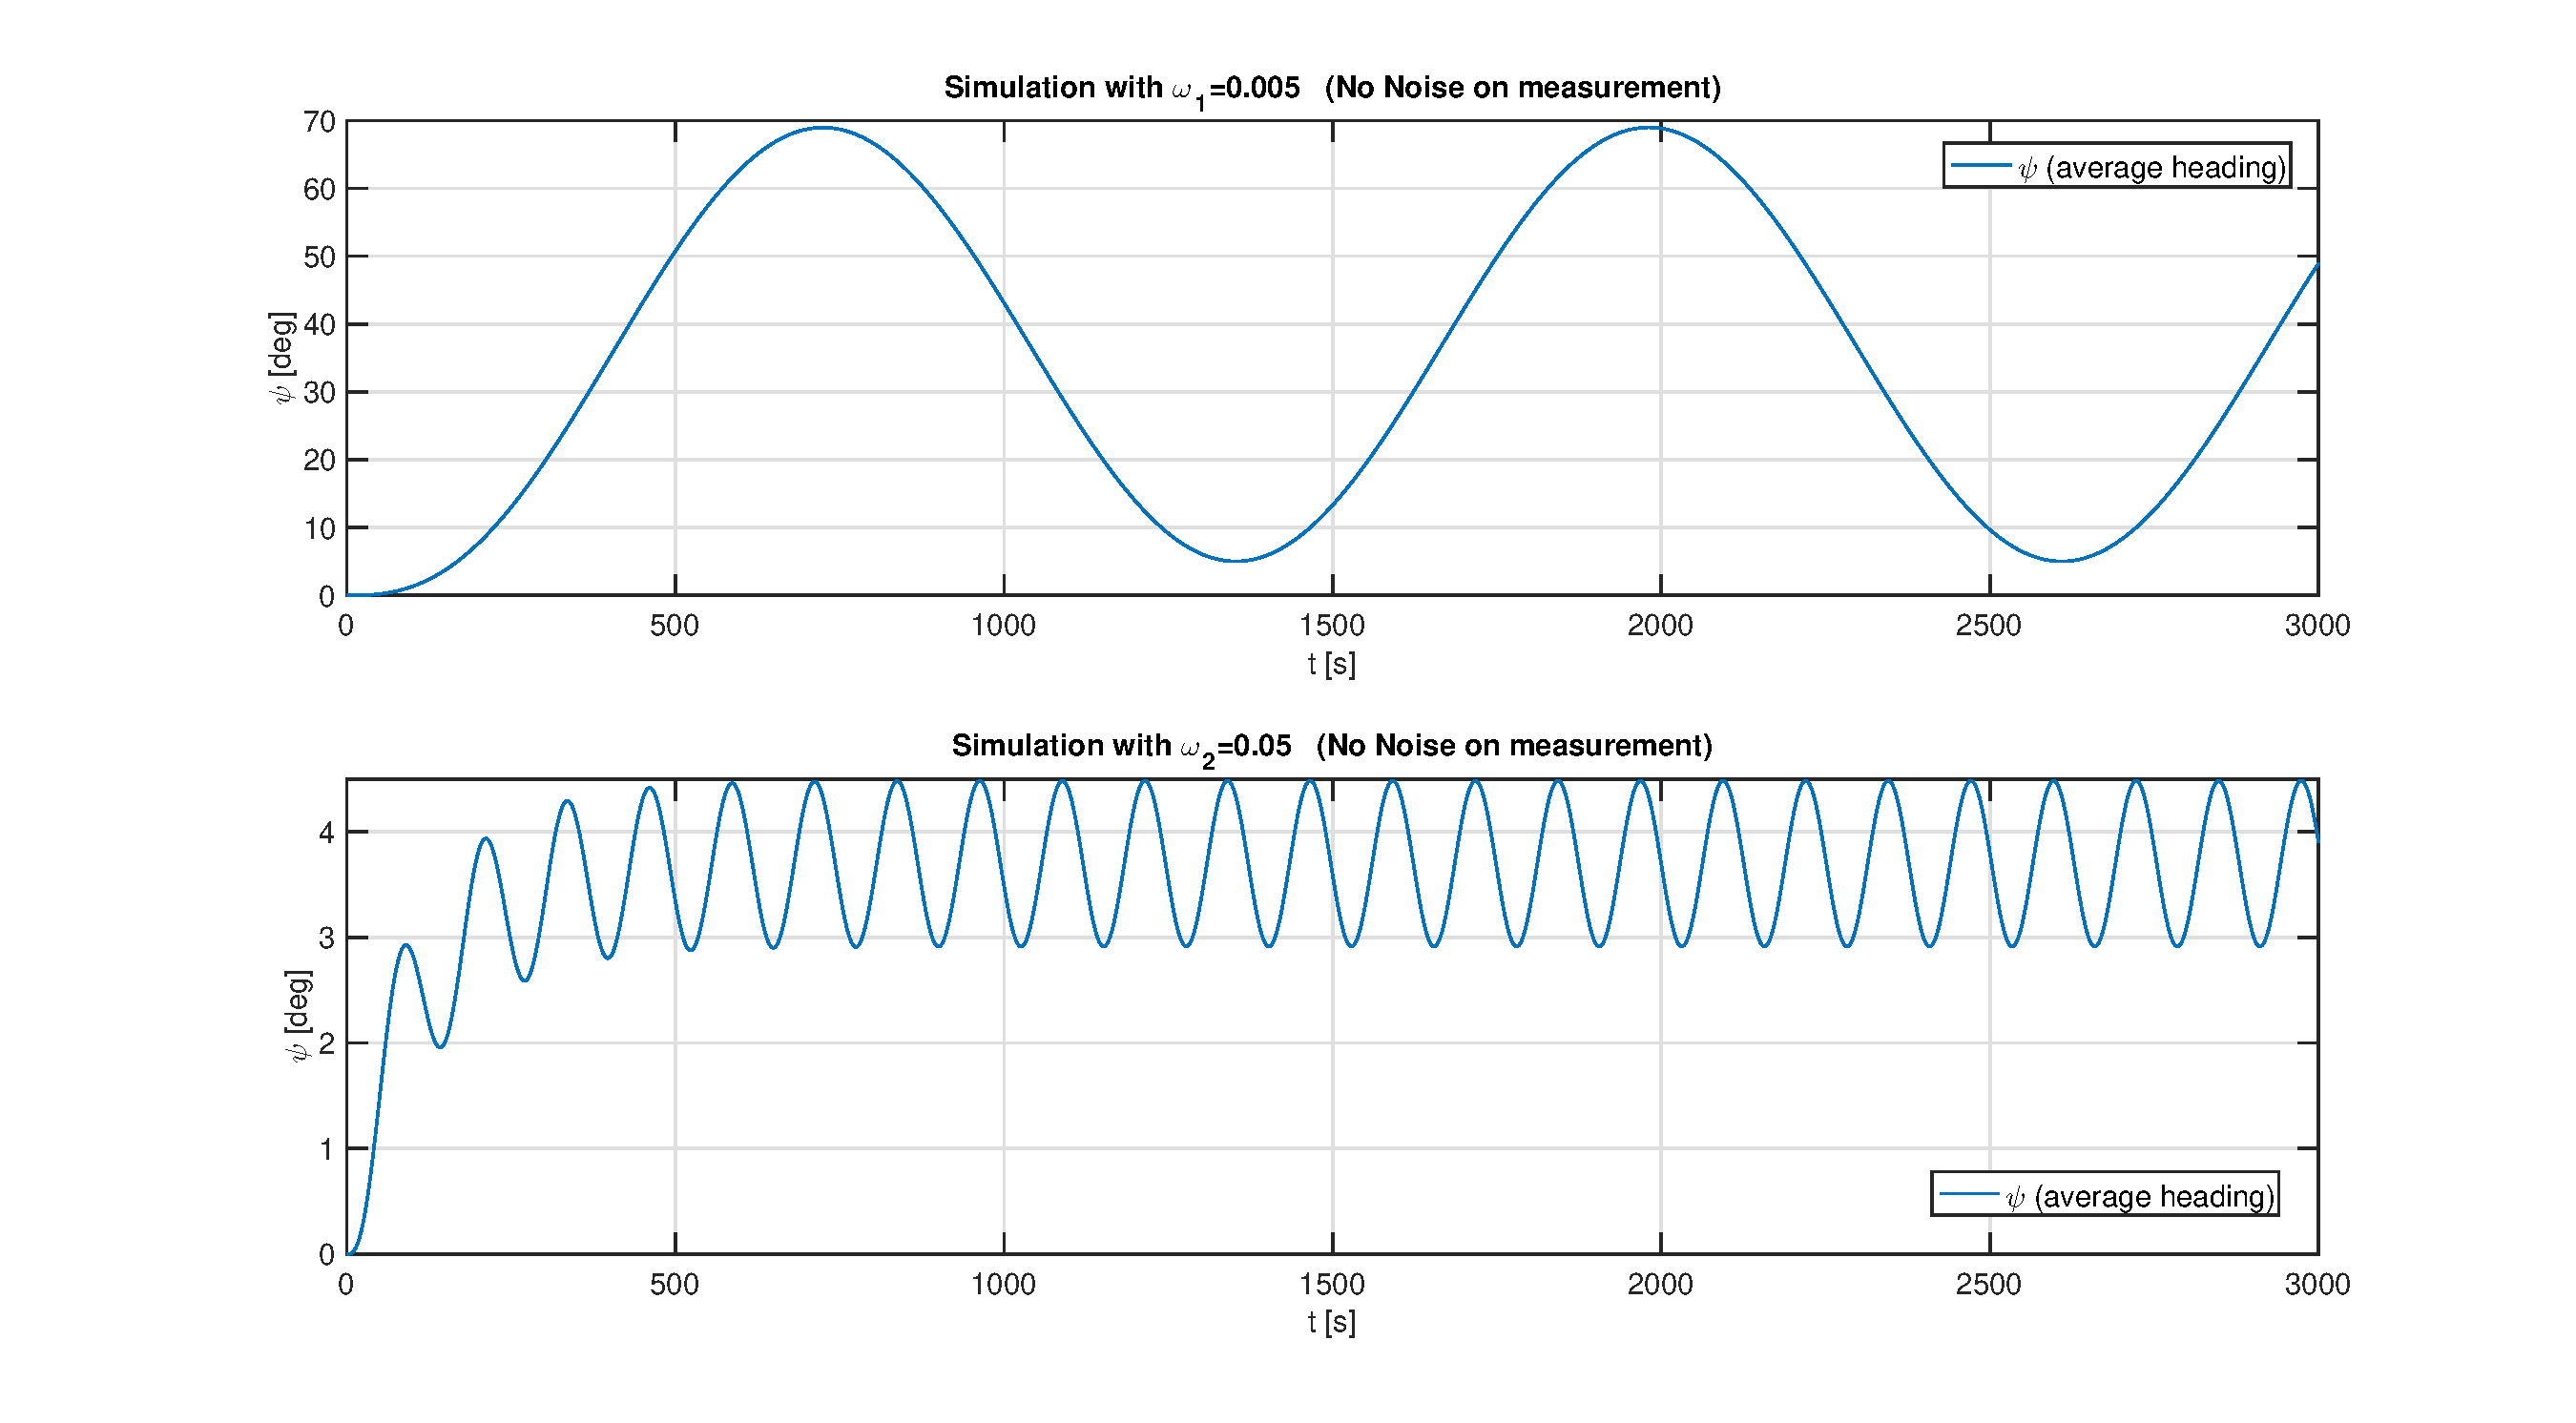
\includegraphics[scale=0.4]{plots/1b}}
\end{figure}





From figure 1 we extract the amplitude of the outputs, respectively $A_{01}$ and $A_{02}$, which are found by reading and inserting the maximum and minimum values as shown below:

\begin{align*}
{A_{{0_1}}}  &= \frac{{68.98 - 5.02}}{2} = 31.98\\
{A_{{0_2}}} &= \frac{{4.48 - 2.92}}{2} = 0.78
\end{align*}

Inserting these values into equation (\ref{T}) and equation (\ref{K_calc}) gives:

\begin{align*}
K  &= 0.1742\\
T &= 86.5268
\end{align*}







%%%%%%%%%%%%%%%%%%%%%%%%%%%%%%%%%%%%%%%%%%%%%%%%%%%%%%%%%%%%%%%%%%%%%%%%
% 1.3 Boat Parameters with Wave and Measurement Noise
%%%%%%%%%%%%%%%%%%%%%%%%%%%%%%%%%%%%%%%%%%%%%%%%%%%%%%%%%%%%%%%%%%%%%%%%
\subsection{Boat Parameters with Wave and Measurement Noise}

In this section, the previous section will be repeated, but with disturbance. The disturbance consists of waves and measurement noise. Figure 2 displays the output when $\omega = \omega_{1}$ and when $\omega = \omega_{2}$.

\begin{figure}[!htb]
    \caption{Average heading with waves and measurment noise, A=1}
    \centering
    \centerline{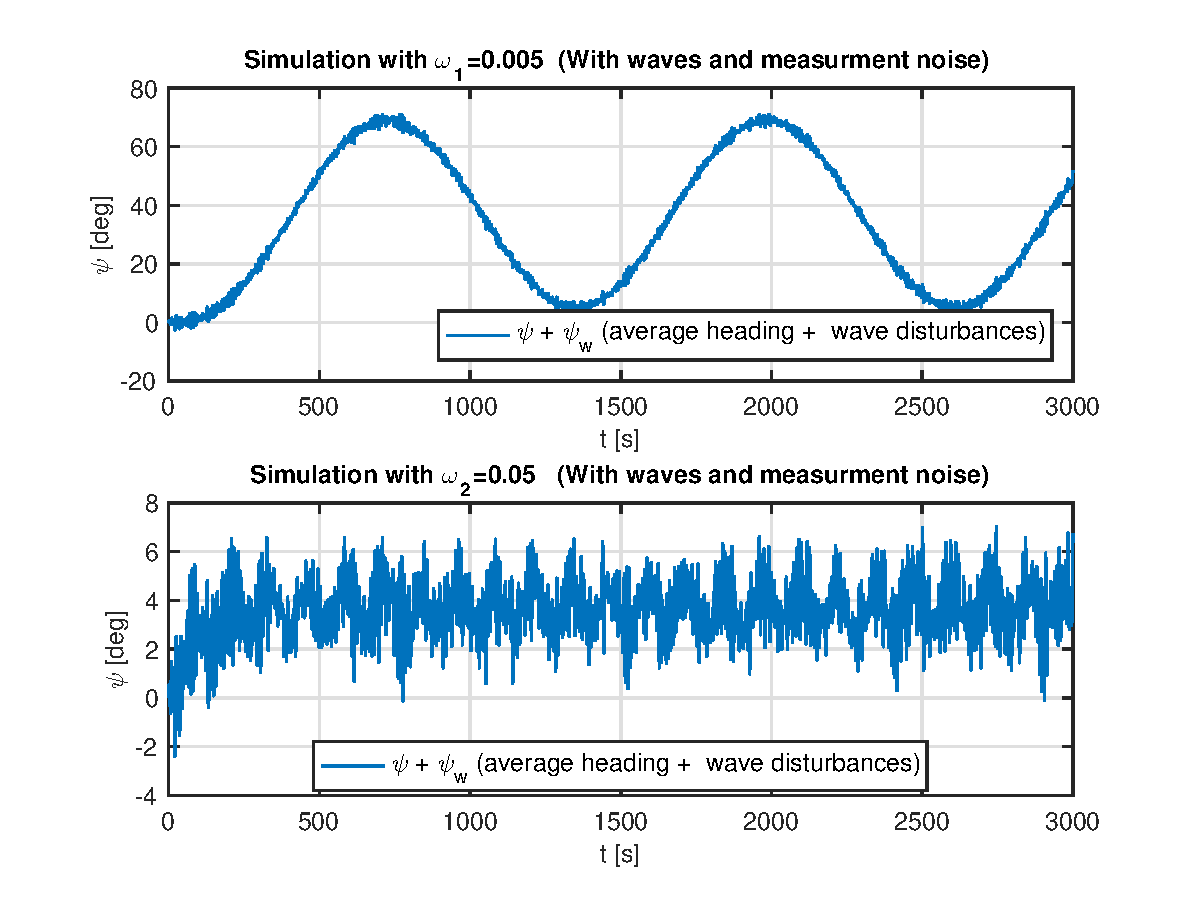
\includegraphics[scale=0.8]{plots/1cA1}}
\end{figure}




From the figure, it is rather difficult to extract any data thus the signal of the noise ratio is low. It is possible though, by using different software tools inside MatLab, but increasing the amplitude of the input signal provided us with the necessary results. An output signal with less noise is obtained by using the following parameters:

\begin{align*}
\omega_1 &= 0.005\\
\omega_2 &= 0.05\\
A &= 45
\end{align*}


\begin{figure}[!htb]
    \caption{Compassion with higher amplitude, A=45}
    \centering
    \centerline{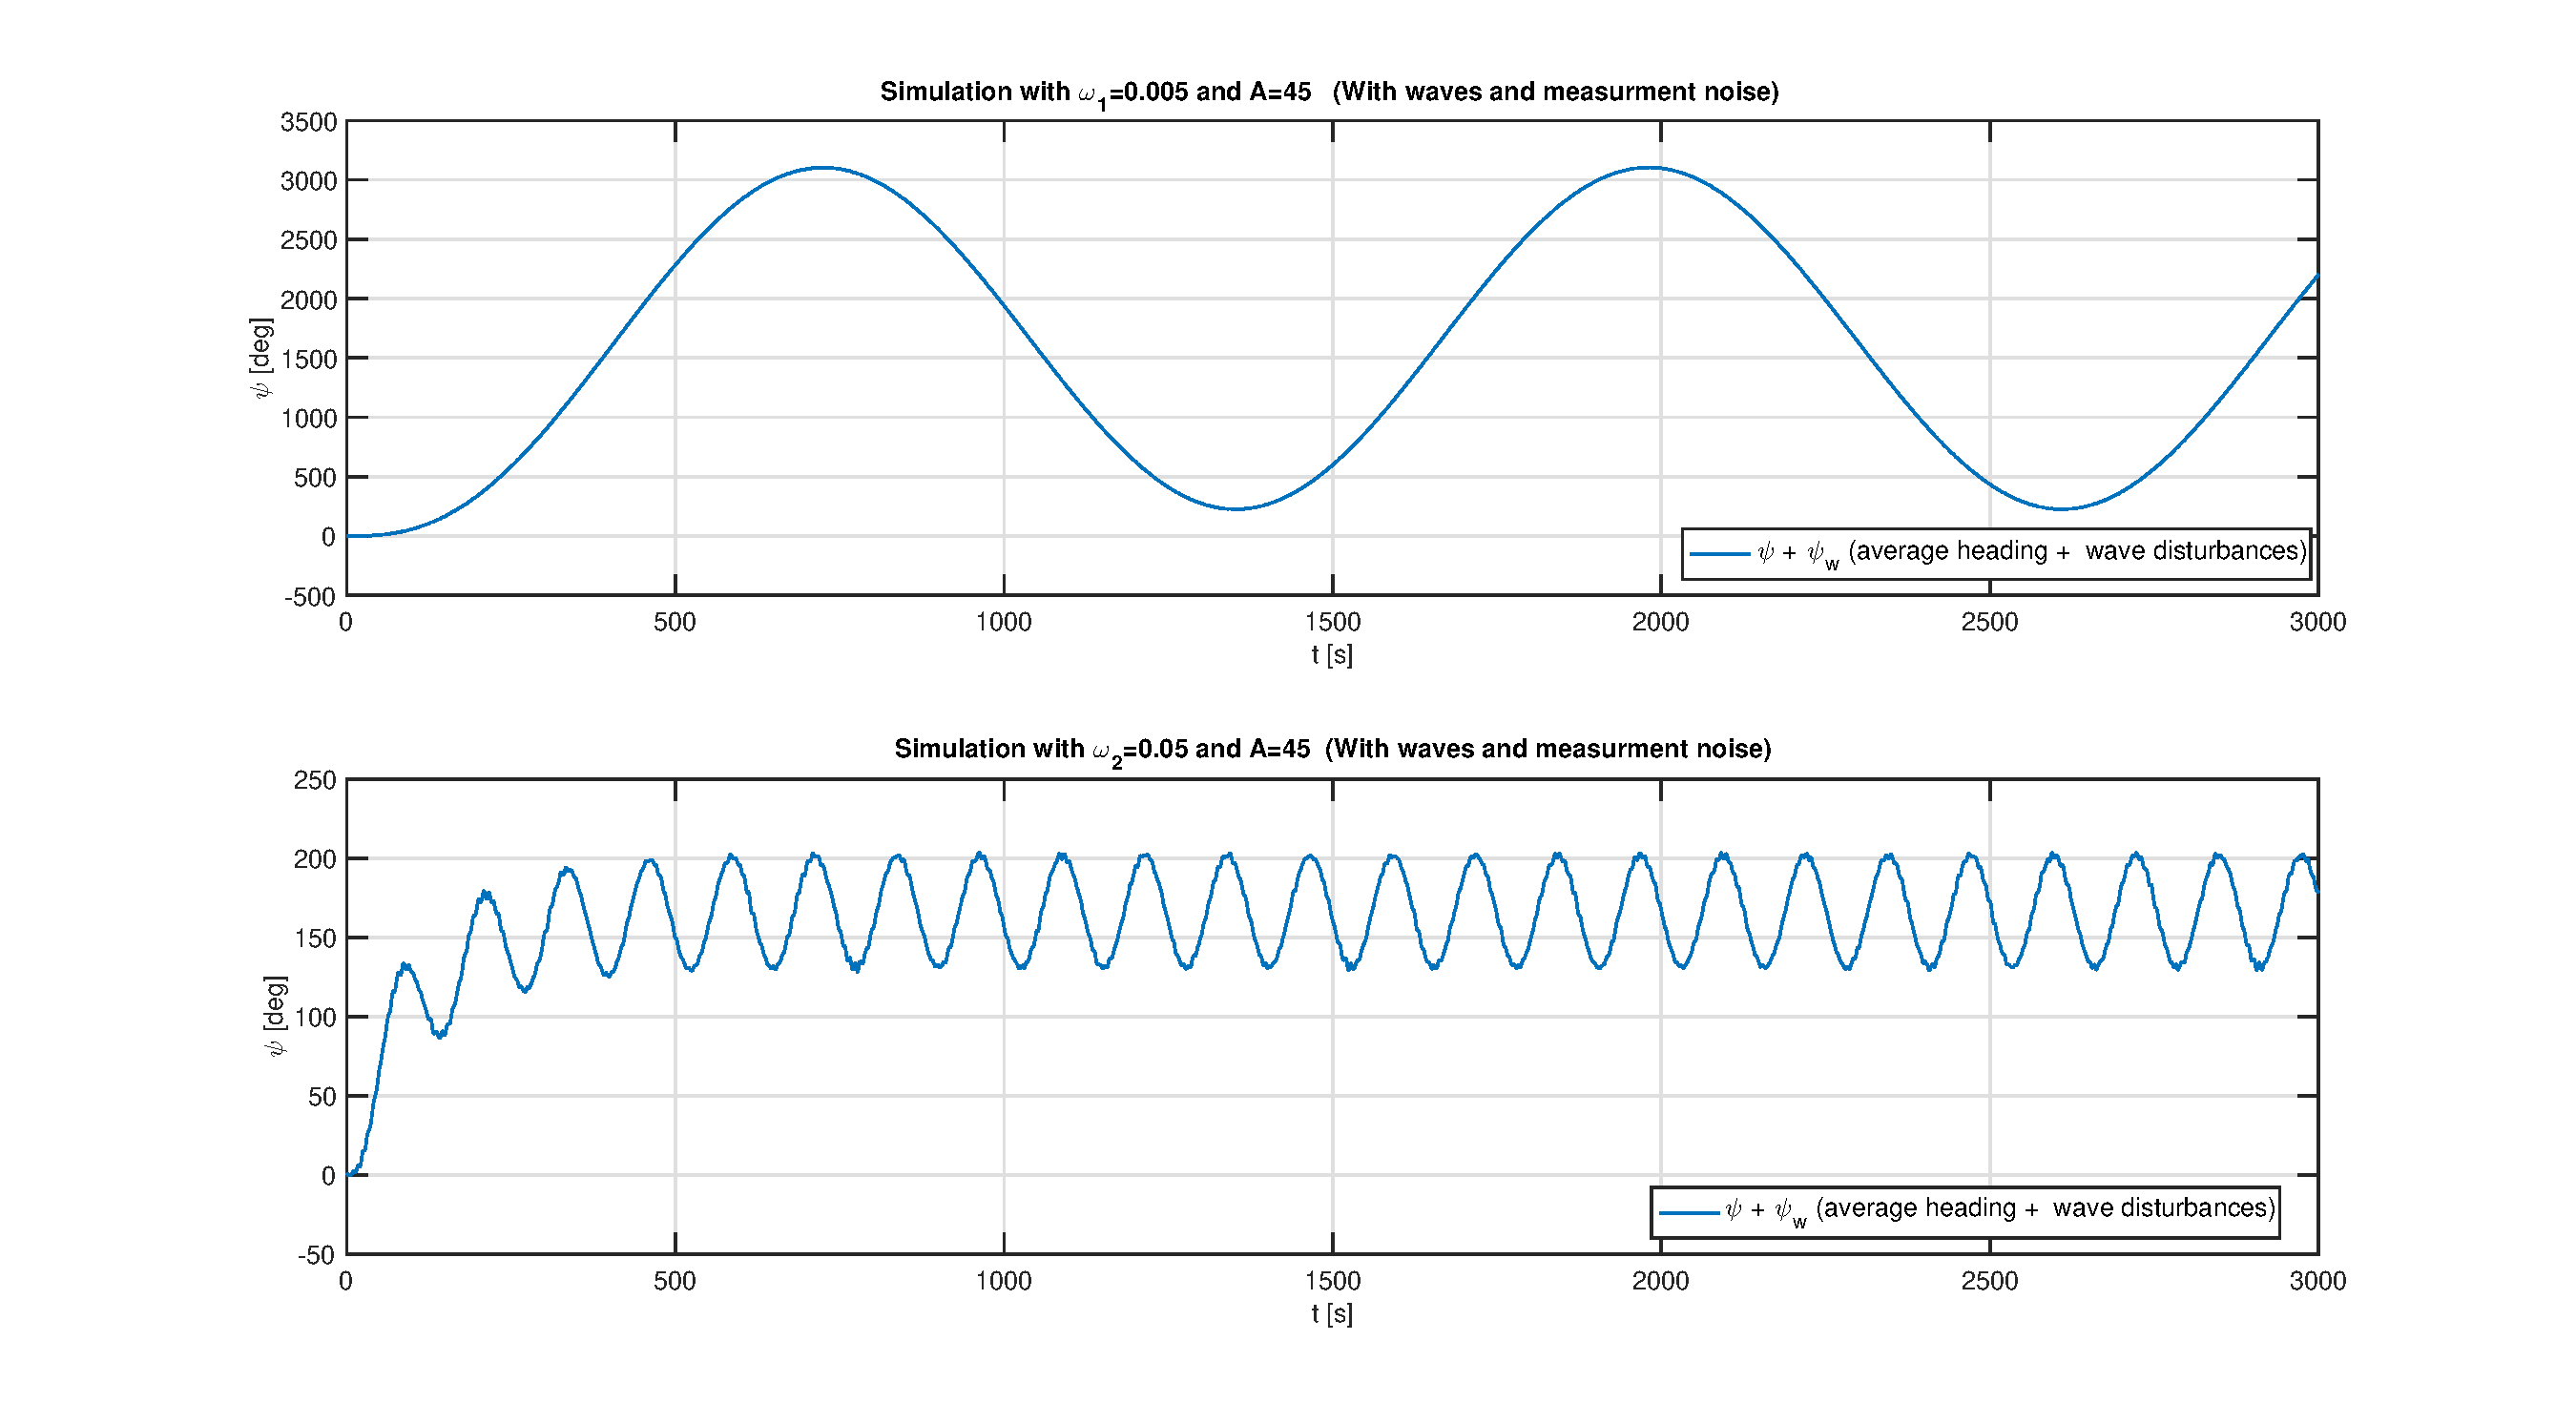
\includegraphics[scale=0.4]{plots/1cA45}}
\end{figure}

These new figures displays a readable format, which is used to calculate the amplitude of the outputs, respectively $A_{01}$ and $A_{02}$.

\begin{align*}
{A_{{0_1}}}  &= \frac{{3105 - 224.5}}{2} = 1440.25\\
{A_{{0_2}}} &= \frac{{202.5 - 130.4}}{2} = 36.05
\end{align*}

Inserting these values into equation (\ref{T}) and equation (\ref{K_calc}) gives:

\begin{align*}
K  &= 0.1734\\
T &= 84.3920
\end{align*}

Comparing these values to what we obtained in section 1.2, we see that the deviation is rather small, less than 2.5\%. The values obtained in section 1.2 are the values that will be used throughout this report.

%%%%%%%%%%%%%%%%%%%%%%%%%%%%%%%%%%%%%%%%%%%%%%%%%%%%%%%%%%%%%%%%%%%%%%%%
% 1.4 Verifying Model Approximation
%%%%%%%%%%%%%%%%%%%%%%%%%%%%%%%%%%%%%%%%%%%%%%%%%%%%%%%%%%%%%%%%%%%%%%%%
\subsection{Verifying Model Approximation}

Figure 4 compares the average heading response $\psi(t)$ of the ship simulation model compared to the estimated model with and without disturbances as a way of simulating weather conditions. The plot shows a good approximation, though the deviation increases with time. Analyzing the plot, it is clear that there is something happening between 300 and 500 seconds, after this the deviation increases and the approximation starts to drift as $t \to \infty $.



%\ref{plot:1d} is displaying the error (${e_\psi }$) of the model compared to the ship. After 450 seconds, error is increasing. $\psi (t)$ is obtained by integrating the yaw rate $r(t)$. Since the comparison displays a good match for at least 450 seconds, we can conclude that the estimated parameters provides a good realistic picture for $r(s)/\delta(s)$.%


\begin{figure}[!htb]
    \caption{Compassion  of model and system}
    \centering
    \centerline{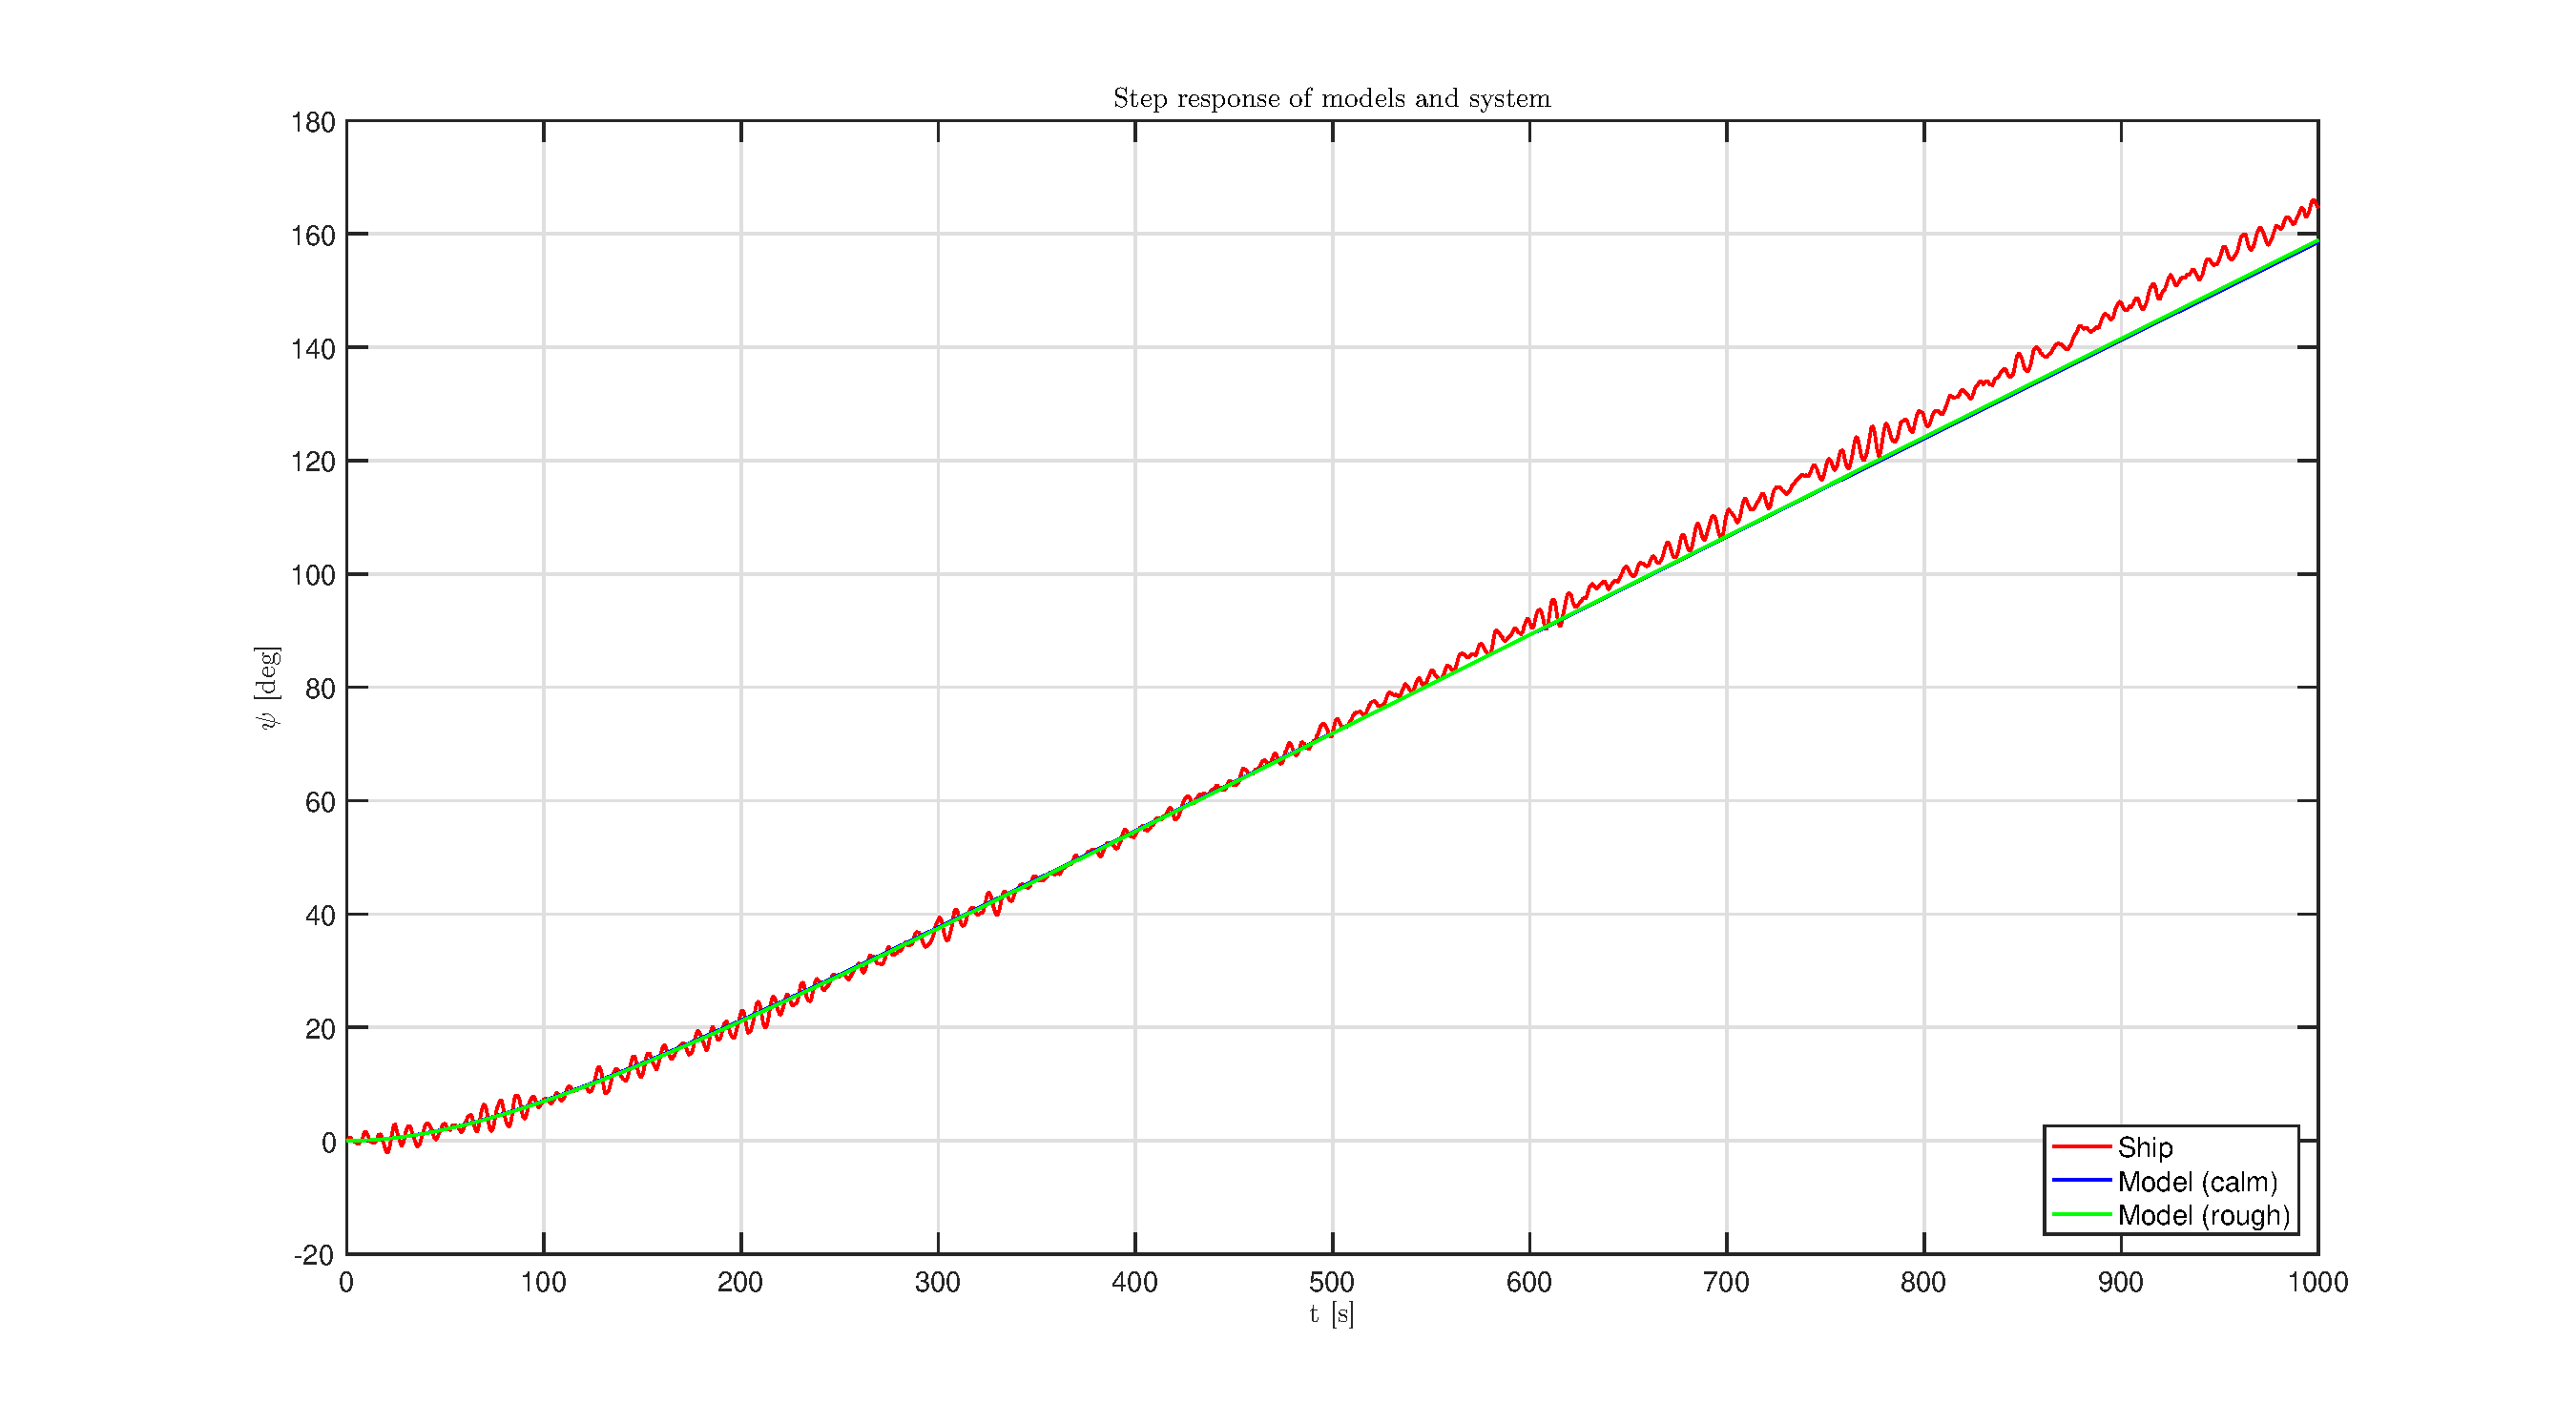
\includegraphics[scale=0.4]{plots/1d}}
    \label{plot:1d}
\end{figure}

\newpage
\section{Identification of Wave Spectrum Model}

In this section the Power Spectral Density (PSD) function, ${P_{{\psi _\omega }}}$ is covered.

%%%%%%%%%%%%%%%%%%%%%%%%%%%%%%%%%%%%%%%%%%%%%%%%%
% 2.1 Power Spectral Density Estimate
%%%%%%%%%%%%%%%%%%%%%%%%%%%%%%%%%%%%%%%%%%%%%%%%%
\subsection{Power Spectral Density Estimate, $S_{\psi_{\omega}}$}

A dataset with how waves have an impact on compass measurements is provided as a time series by ${\psi _\omega }$. To find an estimate for ${S_{{\psi _\omega }}}$ we use the following MatLab script with the function $[pxx, f] = ...pwelch(x, window, noverlap, nfft, fs)$ which utilizes discrete Fourier transform to estimate the PSD function from a time series signal. The function basically returns the two-sided Welch PSD estimates at the frequencies specified in the vector, f. 

\textbf{MatLab-script with \textit{pwelch}:}
\begin{lstlisting}
F_s = 10;
window = 4096;
noverlap = [];
nfft = [];  
[S_psi,f] = pwelch(psi_w(2,:).*(pi/180),window,noverlap,nfft,F_s);
omega = 2*pi.*f;
S_psi = S_psi./(2*pi);  
\end{lstlisting}

\begin{figure}[!htb]
    \caption{PSD Estimate, $S_{\psi_{\omega}}$}
    \centering
    \centerline{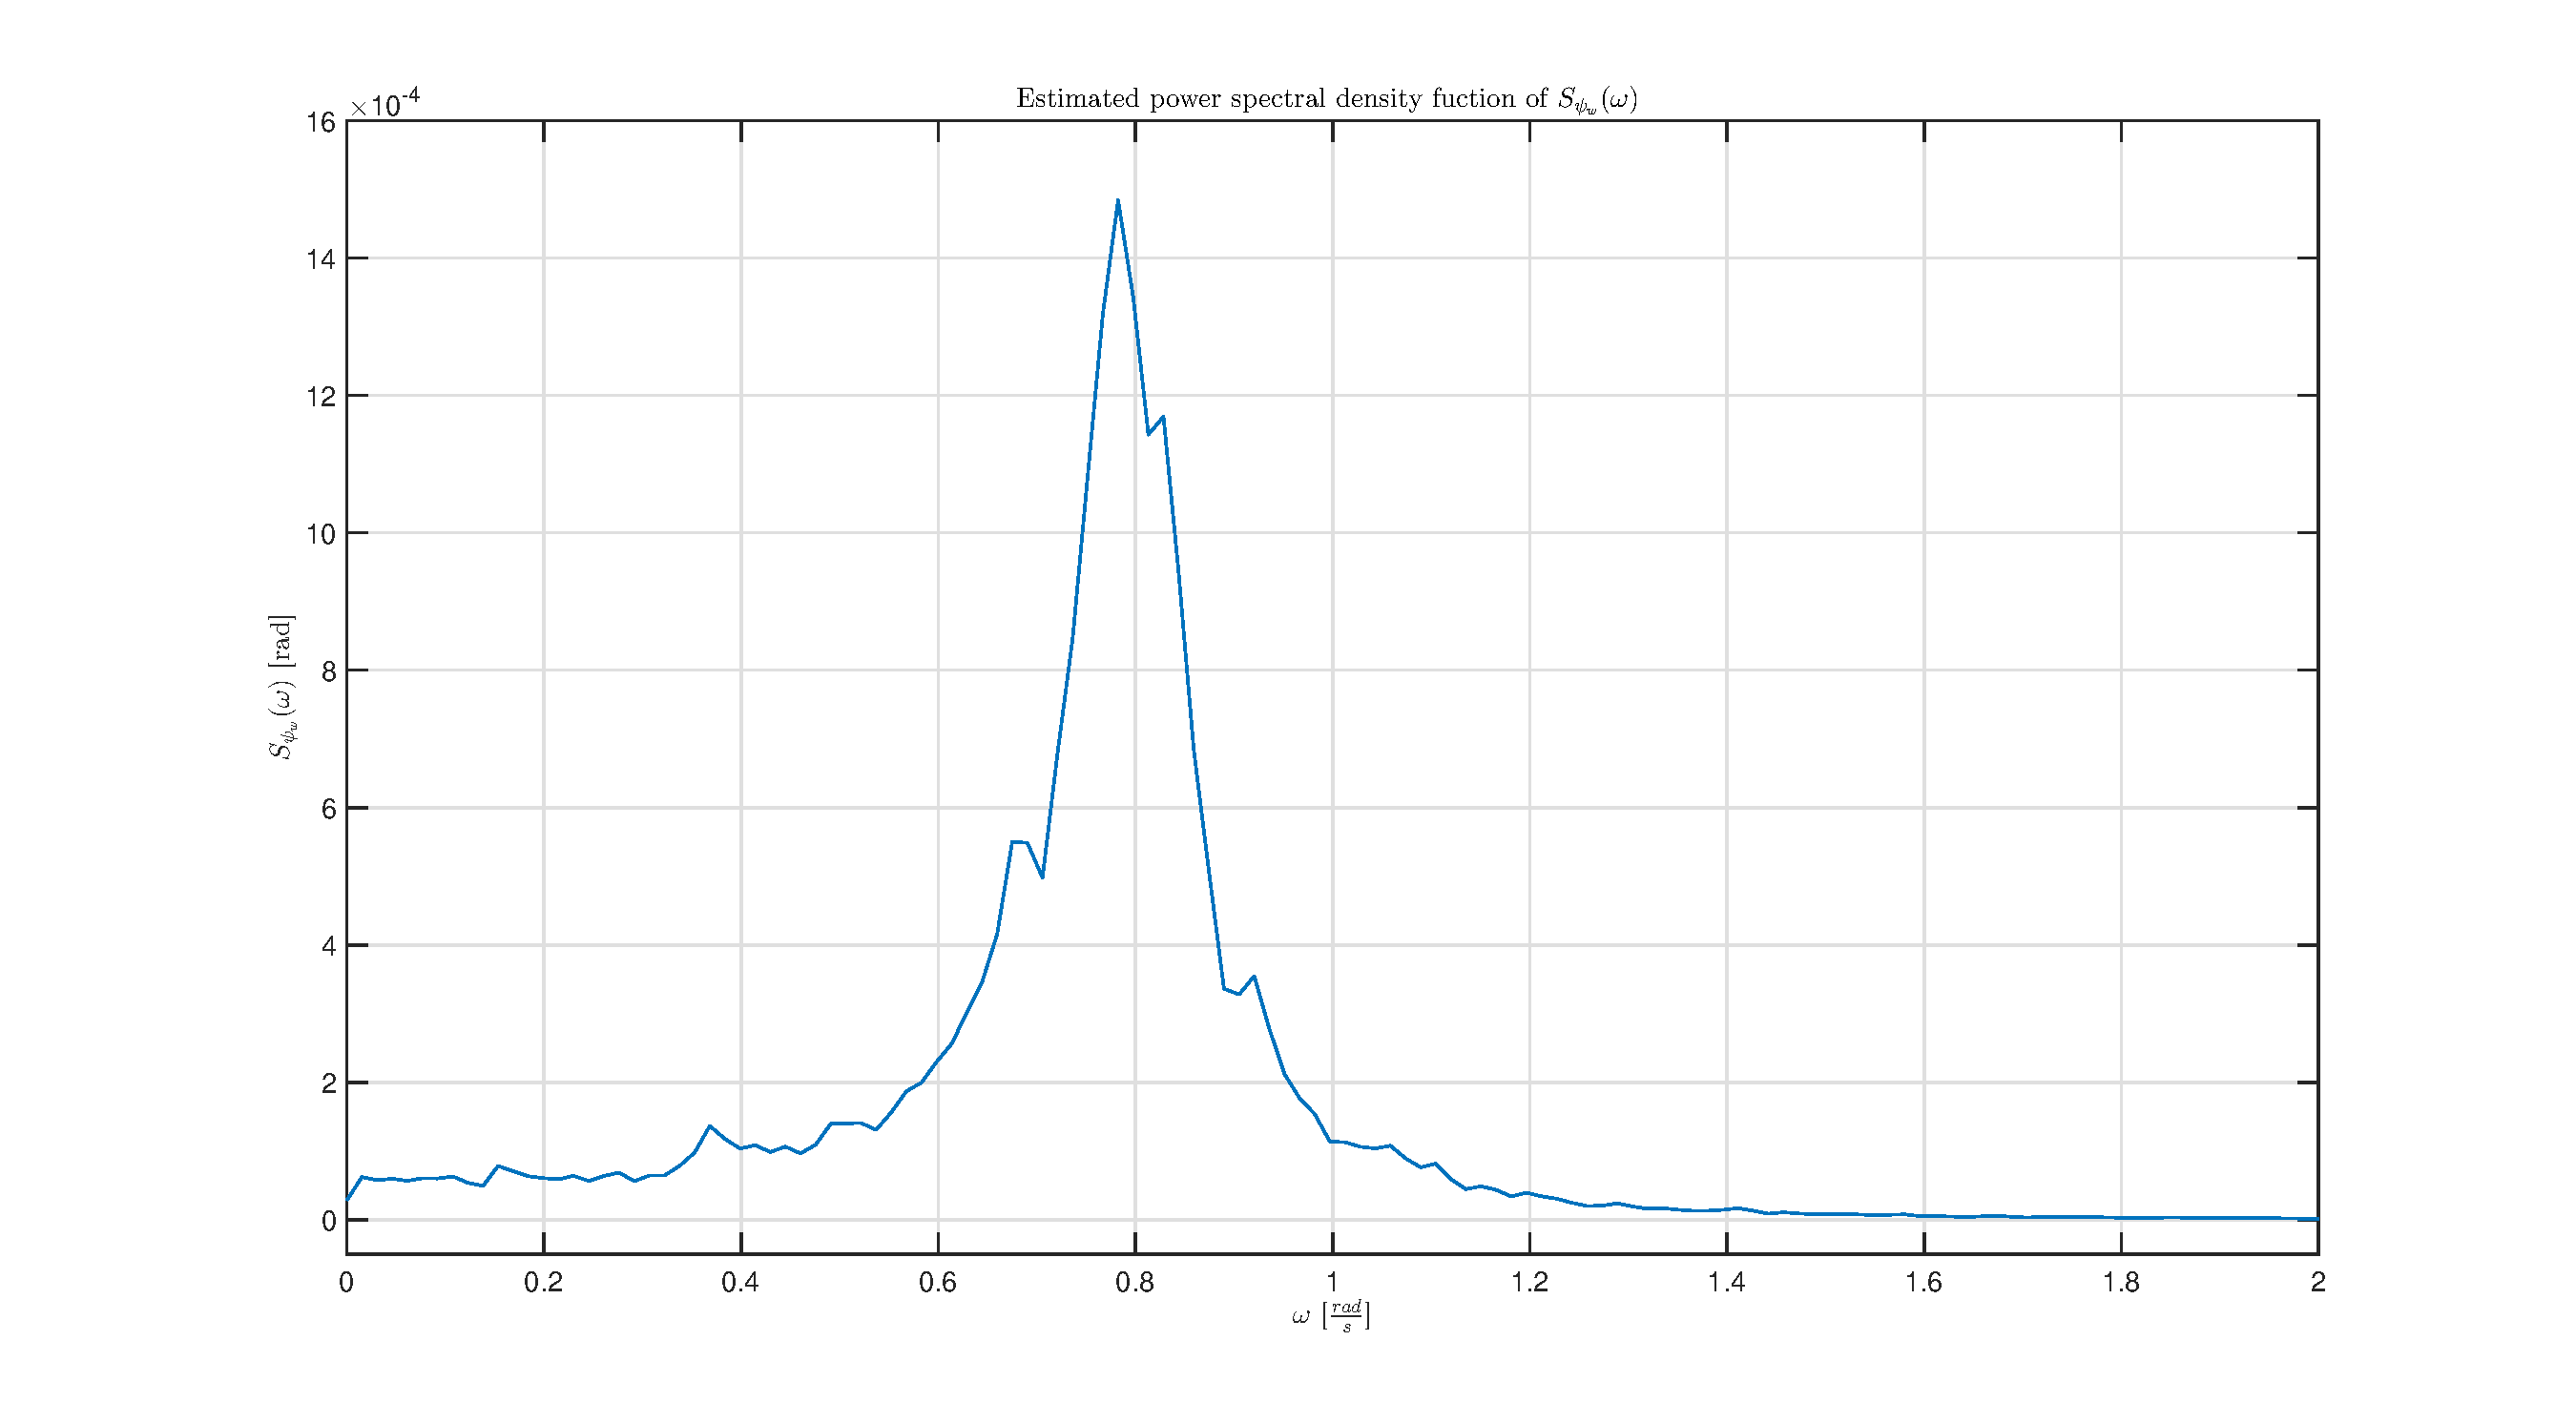
\includegraphics[scale=0.45]{plots/2a}}
    \label{plot:2a}
\end{figure}

%%%%%%%%%%%%%%%%%%%%%%%%%%%%%%%%%%%%%%%%%%%%%%%%%
% 2.2 Analytical Expressions for ${P_{{\psi _\omega }}}$ and ${H_{{\psi _\omega }}}$
%%%%%%%%%%%%%%%%%%%%%%%%%%%%%%%%%%%%%%%%%%%%%%%%%
\subsection{Analytical expressions for ${H_{{\psi _\omega }}}$ and ${P_{{\psi _\omega }}}$}

To obtain the transfer function ${H_{{\psi _\omega }}} = \frac{{{\psi _\omega }}}{{{\omega _\omega }}}$, which describes how the waves affect the yaw angle, we use the model (\ref{model}) as base.

\begin{align}\label{model}
    \begin{array}{l}
    {{\dot \xi }_w} = {\psi _\omega }\\
    {{\dot \psi }_\omega } =  - {\omega _0}^2{\xi _\omega } - 2\lambda {\omega _0}{\psi _\omega } + {K_\omega }{\omega _\omega }
\end{array}
\end{align}

Then Laplace transformation is applied to obtain the transfer function:

\begin{align*}
    \begin{array}{l}
        s\xi  = {\psi _\omega }\\
        s{\psi _\omega } =  - {\omega _0}^2{\xi _\omega } - 2\lambda {\omega _0}{\psi _\omega } + {K_\omega }{\omega _\omega }\\
        s{\psi _\omega } =  - {\omega _0}^2{\psi _\omega }\frac{1}{s} - 2\lambda {\omega _0}{\psi _\omega } + {K_\omega }{\omega _\omega }
\end{array}
\end{align*}

\begin{equation}
    {H_{{\psi _\omega }}} = \frac{{{\psi _\omega }}}{{{\omega _\omega }}} = \frac{{{K_\omega }s}}{{{s^2} + 2\lambda {\omega _0}s + {\omega _0}^2}}
\end{equation}

To find an analytical expression for ${P_{{\psi _\omega }}}$, we use the relationship expressed in (\ref{brown}). ${S_{{\omega _\omega }}}$ is defined by it being \textit{zero mean unity white noise}. This implies that the variance (${\sigma ^2}$) and spectral density (${S_{{\omega _\omega }}}$) are equal to 1.

\begin{equation}\label{brown}
    {P_{{\psi _\omega }}}(j\omega ) = {H_{{\psi _\omega }}}(j\omega ){H_{{\psi _\omega }}}( - j\omega ){S_{{\omega _\omega }}}
\end{equation}

\begin{equation}
    {P_{{\psi _\omega }}}(\omega ) = \frac{{{K_\omega }^2{\omega ^2}}}{{{\omega ^4} + 2(2{\lambda ^2} - 1){\omega _0}^2{\omega ^2} + {\omega _0}^4}}
\end{equation}


%%%%%%%%%%%%%%%%%%%%%%%%%%%%%%%%%%%%%%%%%%%%%%%%%
% 2.3 Finding $\omega_0$
%%%%%%%%%%%%%%%%%%%%%%%%%%%%%%%%%%%%%%%%%%%%%%%%%
\subsection{Finding $\omega_0$}

$\omega_0$ is the base frequency of the noise $\omega_\omega$ - the frequency which has the highest energy. Figure \ref{plot:2a} shows that is around $\frac{\pi}{4} rad/s$. To find the frequency which has the highest energy, the MatLab command \textit{[M, I] = max(A)}. The following MatLab-script were used to find $\omega_0$:

\textbf{Finding $\omega_0$:}
\begin{lstlisting}
[maxPSD, frequency_index] = max(S_psi);
omega_0 = omega(frequency_index);
\end{lstlisting}

Following values were obtained:

\begin{align*}
    \omega_0 &= 0.78233 \frac{{rad}}{s}\\
    \sigma^2 &= 4.8724 \frac{{\deg }}{{\frac{{rad}}{s}}}
\end{align*}



%%%%%%%%%%%%%%%%%%%%%%%%%%%%%%%%%%%%%%%%%%%%%%%%%
% 2.4 Identifying $\lambda$ and fitting $P_{\psi_\omega}$
%%%%%%%%%%%%%%%%%%%%%%%%%%%%%%%%%%%%%%%%%%%%%%%%%
\subsection{Identifying $\lambda$ and fitting $P_{\psi_\omega}$}

To identify the damping factor ($\lambda$), we use curve fitting. Some of the previous calculated values will be used in this identification where we use the MatLab command \textit{x = lsqcurvefit(fun, x0, xdata, ydata, lb, ub)}. \textit{lsqcurvefit} solves non-linear least squares problems. \textit{fun} is a function of \textit{x} and \textit{xdata} where the parameter(s) to be found is \textit{x} and \textit{xdata} is the abscissa data to fit into.

The following script provided $\lambda = 0.086198$.

\textbf{Finding $\lambda$ and $K_{\omega}$:}
\begin{lstlisting}
sigma = sqrt(maxPSD);
P_psi_fun = @(lambda,omega) ...
    (4*lambda^2*omega_0^2*sigma^2*omega.^2) ./ ...
    (omega.^4 + (2*lambda^2 - 1)*2*omega_0^2*omega.^2 + ...
    omega_0^4);

lambda0 = 10;
lb=0;
ub=10;
lambda = lsqcurvefit(P_psi_fun,lambda0,omega,S_psi,lb,ub);
K_w = 2*lambda*omega_0*maxPSD;
P_psi = P_psi_fun(lambda,omega);
\end{lstlisting}


\begin{figure}[!htb]
    \caption{Comparsion}
    \centering
    \centerline{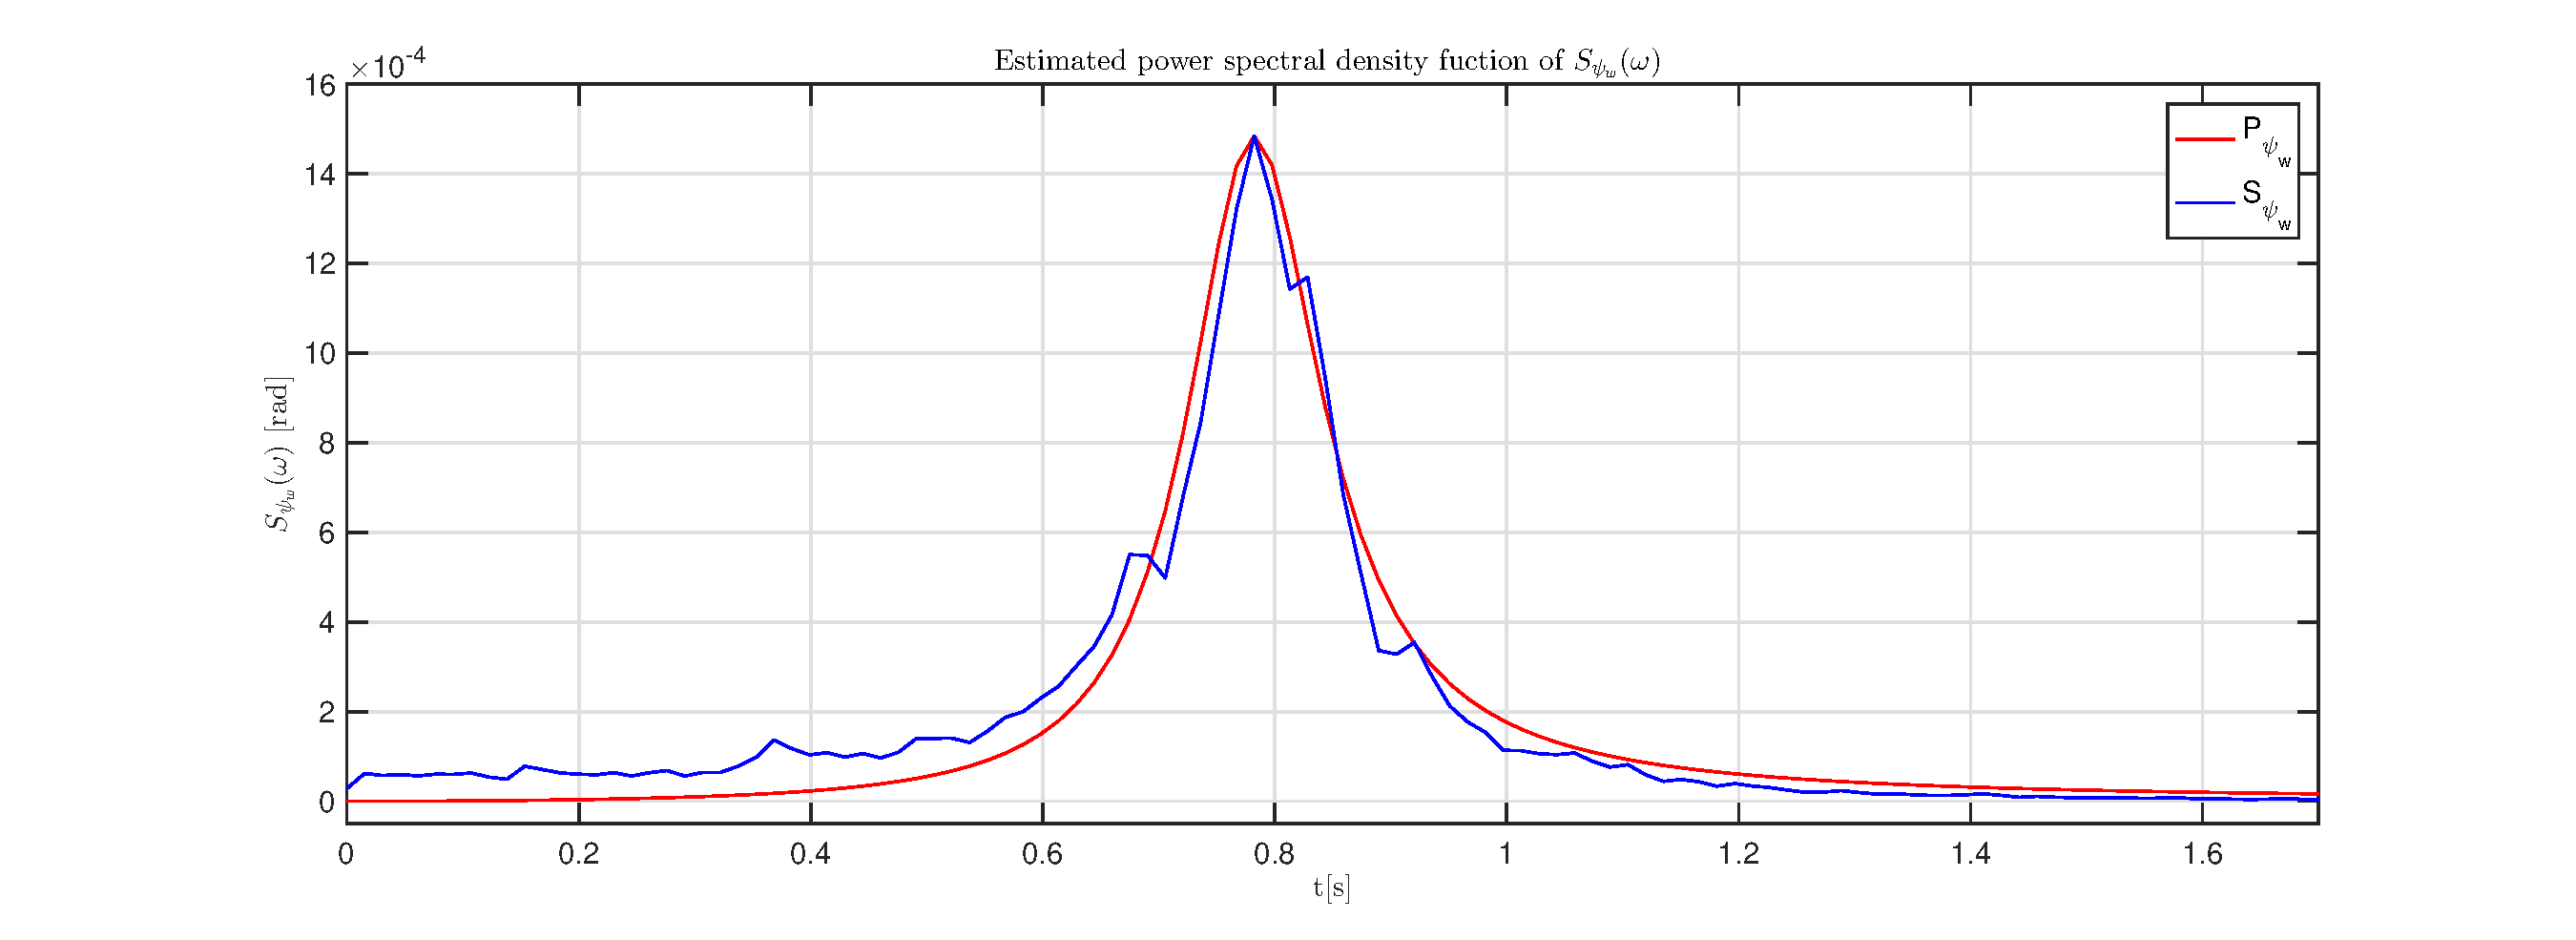
\includegraphics[scale=0.4]{plots/2d}}
\label{plot:2d}
\end{figure}


\newpage
\section{Control System Design}

In this section the autopilot will be developed. The autopilot uses the desired course angle, $\psi_r$ as reference. For the MatLab simulations in this project, $\psi_r = 30^\circ$, as the linearized model only holds for small deviations in $\psi$. 


%%%%%%%%%%%%%%%%%%%%%%%%%%%%%%%%%%%%%%%%%
% PD Controller Design
%%%%%%%%%%%%%%%%%%%%%%%%%%%%%%%%%%%%%%%%%
\subsection{PD Controller Design}

From earlier we had the following equation, which the PD controller is based on:

\begin{equation*}
    H(s) = \frac{{\psi (s)}}{{\delta (s)}} = \frac{K}{{s(Ts + 1)}}
\end{equation*}

This provides the following transfer function for our PD controller:

\begin{equation}
    H_{pd}(s) = K_{pd}\frac{1+T_{d}s}{1+T_{f}s}
\end{equation}

$T_{d}$ is chosen such that the time constant term from the ship transfer function is cancelled, $T_{d} = T$, and we obtain the open-loop transfer function:

\begin{equation}
    H(s) = H_{pd}H_{ship}\frac{K K_{pd}}{T_{f}s^2+s}
\end{equation}

Phase margin and cut-off frequency are respectively chosen to be $\phi = 50^\circ$ and $\omega_{c} = 0.1 rad/s$. These parameters will help us find $K_{pd}$ and $T_{f}$, thus the relationship betweeen cut-off frequency and phase margin are:

\begin{equation}\label{phi}
    \phi  = {180^o} + \angle H(j\omega c)
\end{equation}

\begin{equation}\label{relat}
    1 = H(j\omega c)H( - j\omega c)
\end{equation}

(\ref{phi}) and (\ref{relat}) provide following results for $K_{pd}$ and $T_{f}$:

\begin{equation*}
    {T_f} = \frac{1}{{\tan \phi {\omega _c}}} = 8.391
\end{equation*}

\begin{equation*}
    {K_{pd}} = \sqrt {\frac{{{T_f}^2{\omega _c}^4 + {\omega _c}^2}}{{{K^2}}}}  = 0.7493
\end{equation*}

The Bode diagram in Figure \ref{plot:3a} shows the results obtained.
%%%% FIGURE %%%%%

\begin{figure}[!htb]
    \caption{Bode diagram}
    \centering
    \centerline{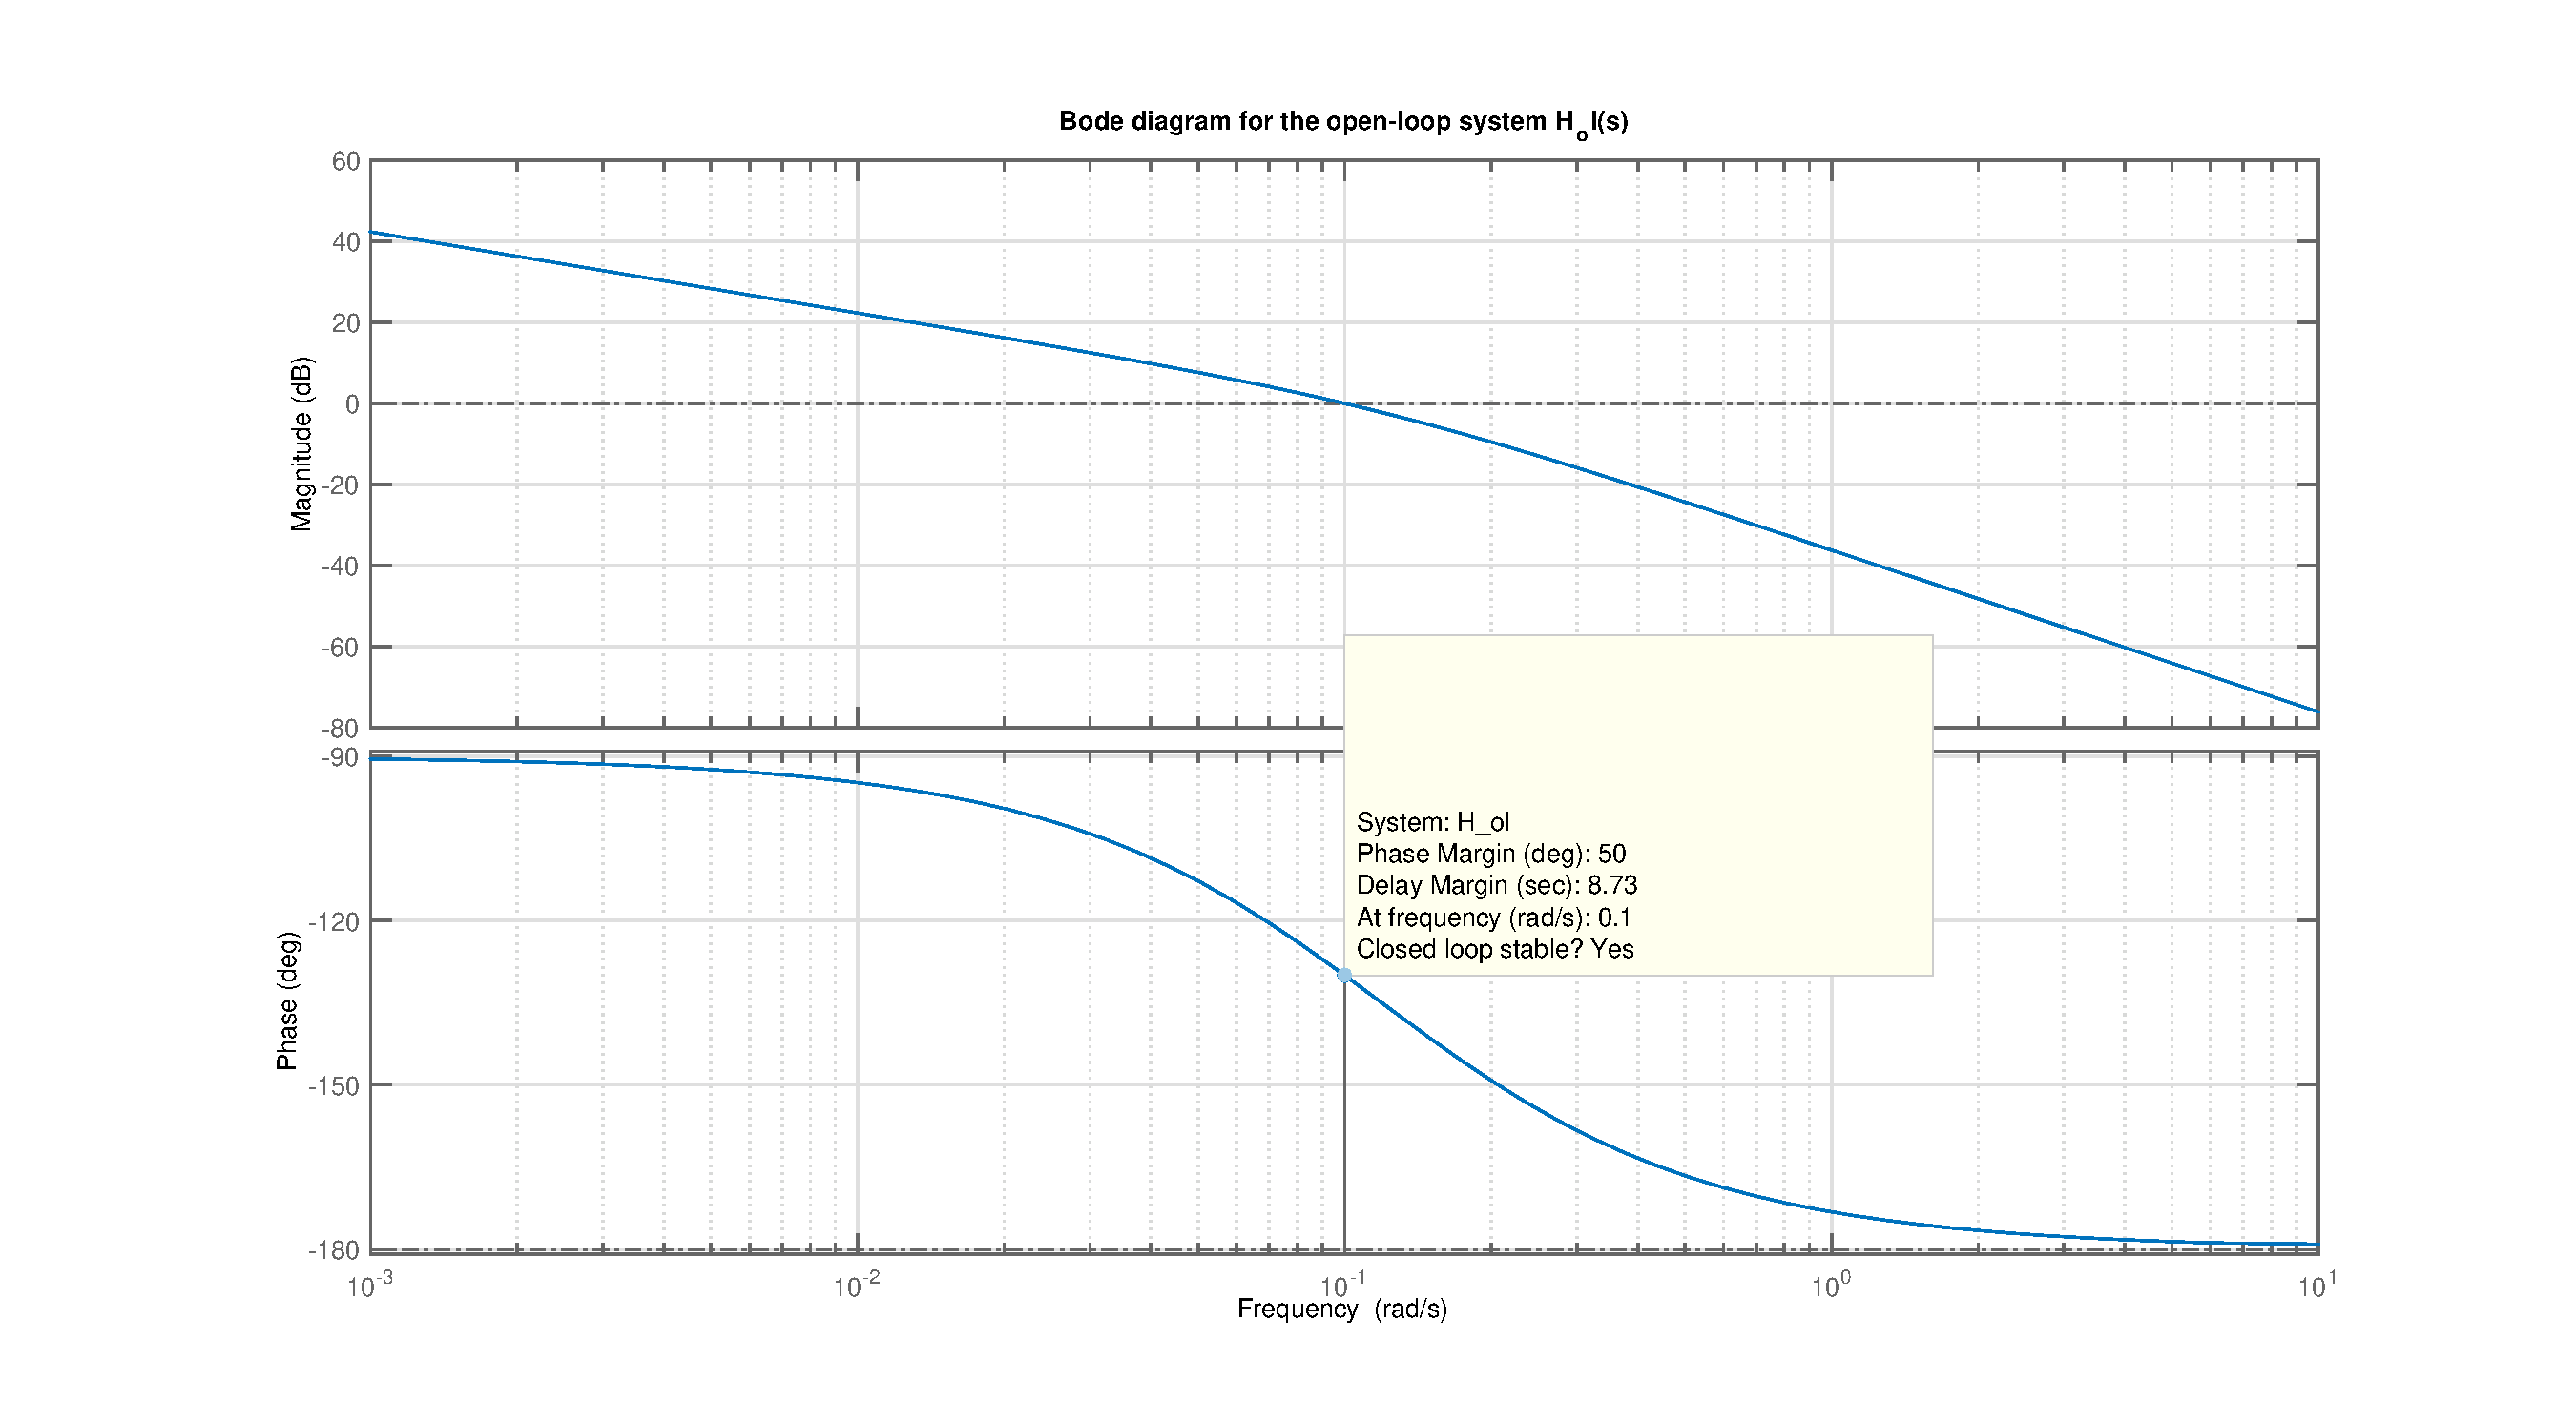
\includegraphics[scale=0.35]{plots/3a}} %This graph is simply too big, i'll fix later.
\label{plot:3a}
\end{figure}

\newpage
%%%%%%%%%%%%%%%%%%%%%%%%%%%%%%%%%%%%%%%%%
% Simulating without disturbances
%%%%%%%%%%%%%%%%%%%%%%%%%%%%%%%%%%%%%%%%%
\subsection{Simulating without disturbances}

In figure \ref{plot:3b} the system simulated without any form of disturbance is displayed. The system is overdamped, but hence its fast convergence to the reference it is only slightly overdamped. The plot of the rudder angle ($\delta$) shows that the actuation is noisy, caused by measurement noise. This might cause undesirable wear on the rudder. 

%%% FIGURE %%%%
\begin{figure}[!htb]
    \caption{Autopilot without disturbances}
    \centering
    \centerline{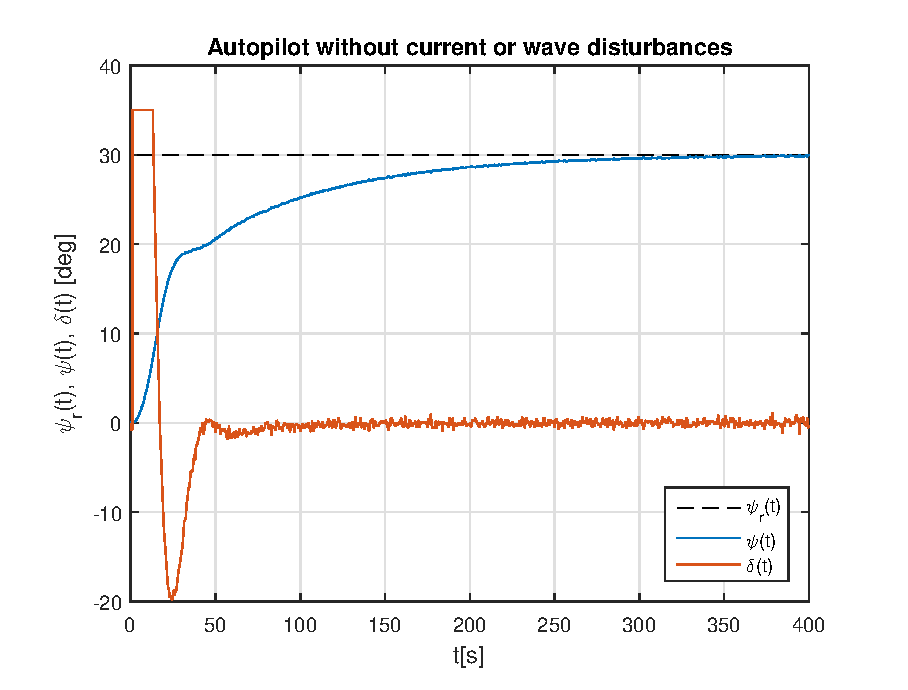
\includegraphics[scale=0.8]{plots/3b}} %This graph is simply too big, i'll fix later.
    \label{plot:3b}
\end{figure}

\newpage
%%%%%%%%%%%%%%%%%%%%%%%%%%%%%%%%%%%%%%%%%
% Simulating with current disturbance
%%%%%%%%%%%%%%%%%%%%%%%%%%%%%%%%%%%%%%%%%
\subsection{Simulating with current disturbance}

This system is simulated with a current disturbance, displayed in figure \ref{plot:3c}. In the model, the effect of the current is a rudder angle bias ($b$). The rudder angle bias ($b$) gives the system a steady-state error, since there is no feed forward or integral action in the controller.

%%%%% FIGURE %%%%%%
\begin{figure}[!htb]
    \caption{Autopilot with current disturbances}
    \centering
    \centerline{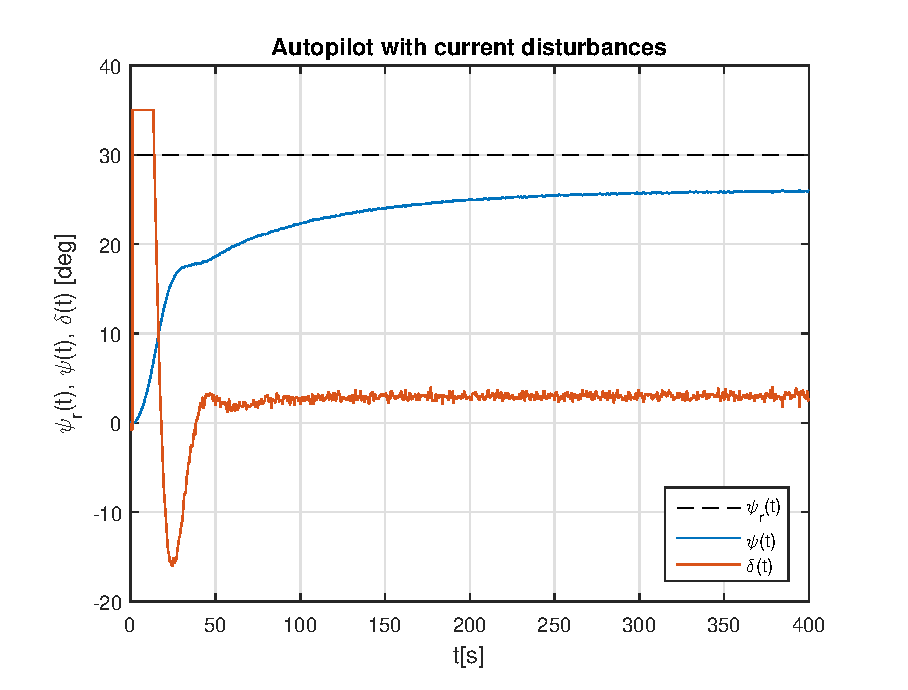
\includegraphics[scale=0.8]{plots/3c}} %This graph is simply too big, i'll fix later.
\label{plot:3c}
\end{figure}

\newpage
%%%%%%%%%%%%%%%%%%%%%%%%%%%%%%%%%%%%%%%%%
% Simulating with wave disturbance
%%%%%%%%%%%%%%%%%%%%%%%%%%%%%%%%%%%%%%%%%
\subsection{Simulating with wave disturbance}

In figure \ref{plot:3d} the system simulated with wave disturbance is displayed. The waves cause a disturbance on the yaw angle ($\psi_{\omega}$). This disturbance is of high frequency with relative high amplitude, which makes the actuation of the rudder noisy. 

%%%% FIGURE %%%%%%%

\begin{figure}[!htb]
    \caption{Autopilot with wave disturbances}
    \centering
    \centerline{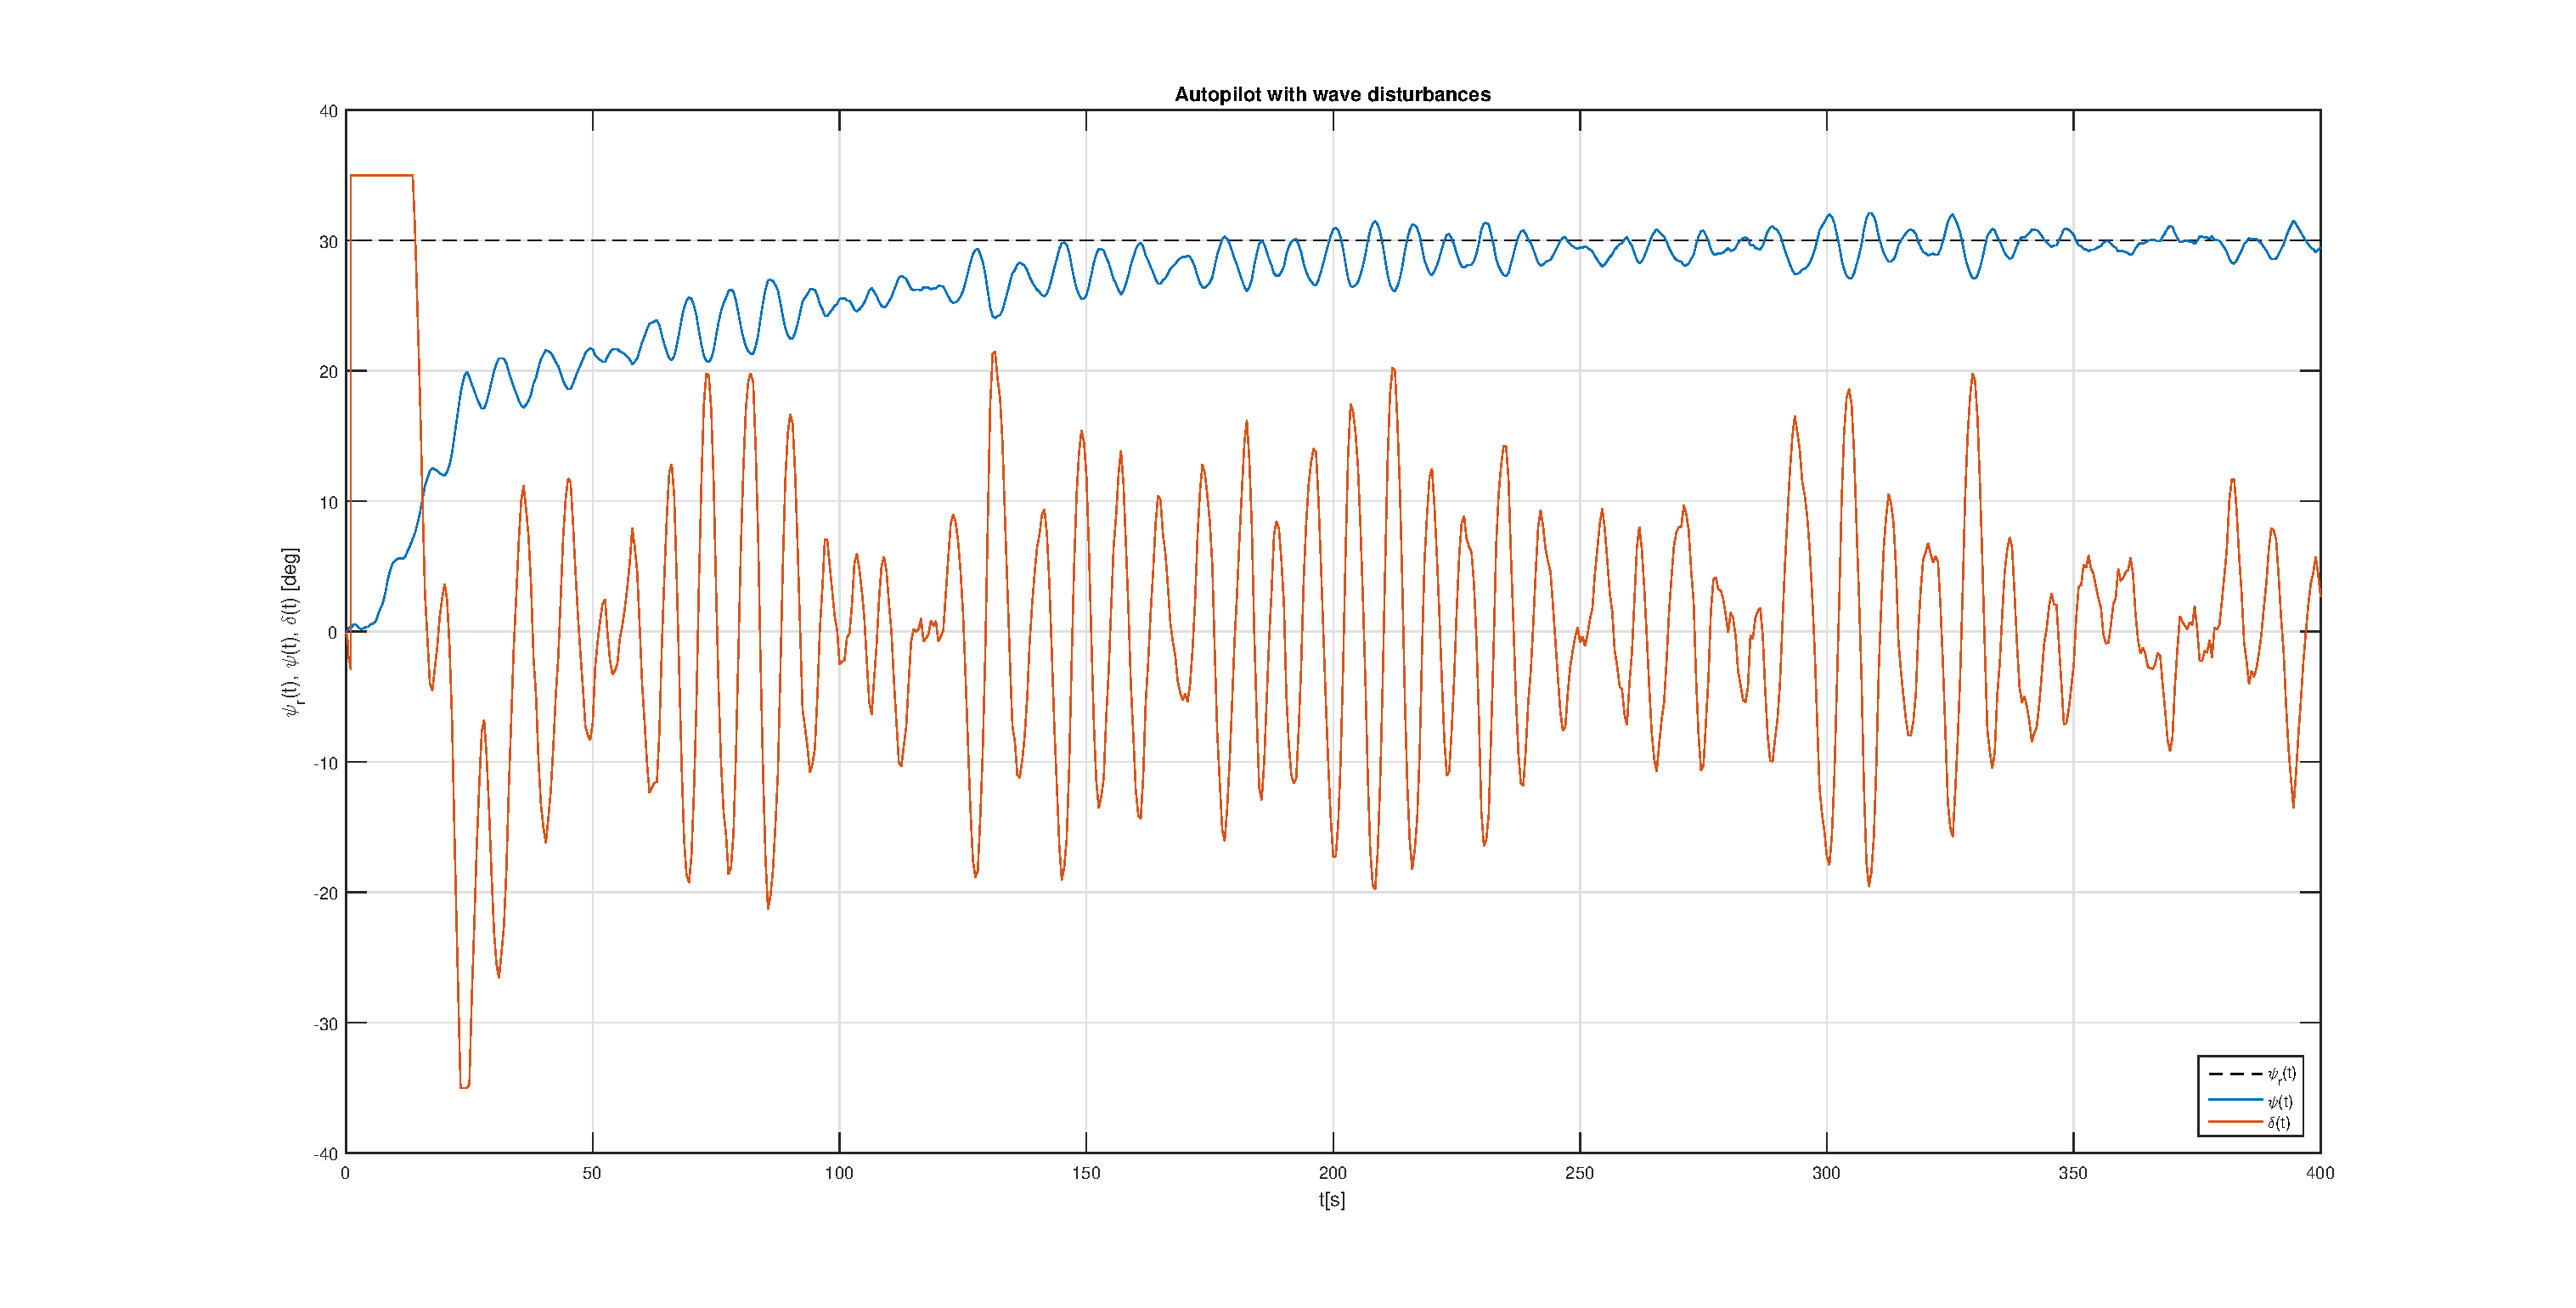
\includegraphics[scale=0.3]{plots/3d}} %This graph is simply too big, i'll fix later.
\label{plot:3d}
\end{figure}
\newpage
\section{Observability}

%%%%%%%%%%%%%%%%%%%%%%%%
% 4.1 Derivation of State Space Matrices
%%%%%%%%%%%%%%%%%%%%%%%%
\subsection{Derivation of State Space Matrices}
The derivation of the State Space Matrices is done with the state vector, input and disturbance as shown here:
\begin{equation}\label{state vector}
\begin{array}{ccc}
     x = \left[ {\begin{array}{*{20}{c}}
{{\xi _\omega }}\\
{{\psi _\omega }}\\
\psi \\
r\\
b
\end{array}} \right],&  
    u = \delta  ,&  
    \omega  = \left[ {\begin{array}{*{20}{c}}
    {{\omega _\omega }}\\
    {{\omega _b}}
\end{array} }\right] 
\end{array}
\end{equation}

We have the following model:
\begin{align}
    \begin{array}{l}
{{\dot \xi }_2} = {\psi _\omega }\\
{{\dot \psi }_\omega } =  - {\omega _0}^2{\xi _\omega } - 2\lambda {\omega _0}{\psi _\omega } + {K_\omega }{\omega _\omega }\\
\dot \psi  = r\\
\dot r =  - \frac{1}{T} + \frac{K}{T}(\delta  - b)\\
\dot b = {\omega _b}\\
y = \psi  + {\psi _\omega } + v
\end{array}
\end{align}

The system can be written as:

\begin{equation}
\begin{array}{cc}
    \dot{x} = \left[ {\begin{array}{*{20}{c}}
{{x_2}}\\
{ - {\omega _0}^2{x_1} - 2\lambda {\omega _0}{x_2} + {K_\omega }{\omega _1}}\\
{{x_4}}\\
{ - \frac{1}{T}{x_4} - \frac{K}{T}{x_5} + \frac{K}{T}u}\\
{{\omega _2}}
\end{array}} \right] ,&  
    y = {x_2}{x_3} + v  
\end{array}
\end{equation}

This corresponds to a system on the following form:

\begin{equation}
   \begin{array}{l}
\dot x = Ax + Bu + E\omega \\
y = Cx + v
\end{array}
\end{equation}

with matrices:
\begin{equation*}\label{matrices}
   \begin{array}{cccc}
       A = \left[ {\begin{array}{*{20}{c}}
0&1&0&0&0\\
{ - {\omega _0}^2}&{ - 2\lambda {\omega _0}}&0&0&0\\
0&0&0&1&0\\
0&0&0&{ - \frac{1}{T}}&{ - \frac{K}{T}}\\
0&0&0&0&0
\end{array}} \right] ,&
       B = \left[ {\begin{array}{*{20}{c}}
0\\
0\\
0\\
{\frac{K}{T}}\\
0
\end{array}} \right] ,& \\\\
       E = \left[ {\begin{array}{*{20}{c}}
0&0\\
{{K_\omega }}&0\\
0&0\\
0&0\\
0&1
\end{array}} \right] ,&
       C = \left[ {\begin{array}{*{20}{c}}
0&1&1&0&0
\end{array}} \right]
   \end{array}
\end{equation*}

To check the observability of the system, we use these following parameters that were calculated in previous sections:

\begin{equation}
   \begin{array}{l}
K = 0.1742\\
T = 86.5268\\
{\omega _0} = 0.7823\\
\lambda  = 0.0862
\end{array}
\end{equation}


%%%%%%%%%%%%%%%%%%%%%%%%
% 4.2 Observability without Disturbances
%%%%%%%%%%%%%%%%%%%%%%%%
\subsection{Observability without disturbances}
Without disturbances, both the state vector from equation  (\ref{state vector}) and the matrices A and C are rewritten as:

\begin{equation}
   x = \left[ {\begin{array}{*{20}{c}}
\psi \\
r
\end{array}} \right]
\end{equation}

\begin{equation*}
   \begin{array}{cc}
       A = \left[ {\begin{array}{*{20}{c}}
0&1\\
0&{ - \frac{1}{T}}
\end{array}} \right] ,&  
       C = \left[ {\begin{array}{*{20}{c}}
1&0
\end{array}} \right]  
   \end{array}
\end{equation*}

This provides an observability matrix which has a rank of 2, meaning the system is observable.

\begin{equation}
   \mathbf{\math\mathcal{O}} = \left[ {\begin{array}{*{20}{c}}
1&0\\
0&1
\end{array}} \right]
\end{equation}


%%%%%%%%%%%%%%%%%%%%%%%%
% 4.3 Observability with current disturbance
%%%%%%%%%%%%%%%%%%%%%%%%
\subsection{Observability with current disturbance}
When current disturbance is applied, it is necessary to rewrite both the state vector and the matrices A and C again, on the form:

\begin{equation}
    x = \left[ {\begin{array}{*{20}{c}}
\psi \\
r\\
b
\end{array}} \right]
\end{equation}

\begin{equation}
    \begin{array}{cc}
       A = \left[ {\begin{array}{*{20}{c}}
0&1&0\\
0&{ - \frac{1}{T}}&{ - \frac{K}{T}}\\
0&0&0
\end{array}} \right] ,&  
       C = \left[ {\begin{array}{*{20}{c}}
1&0&0
\end{array}} \right] 
    \end{array}
\end{equation}

The observability matrix for the system with current disturbance is given by (\ref{observer}), and by using the MatLab command $rank(Ob)$, we can see that it has full row rank of 3, meaning the system is observable.

\begin{equation*}
    \mathbf{\math\mathcal{O}} = \left[ {\begin{array}{*{20}{c}}
1&0&0\\
0&1&0\\
0&{ - \frac{1}{T}}&{ - \frac{K}{T}}
\end{array}} \right]
\end{equation*}

\begin{equation}\label{observer}
    \mathbf{\math\mathcal{O}} = \left[ {\begin{array}{*{20}{c}}
1&0&0\\
0&1&0\\
0&{ - 0.0116}&{ - 0.0020}
\end{array}} \right]
\end{equation}


%%%%%%%%%%%%%%%%%%%%%%%%
% 4.4 Observability with wave disturbance
%%%%%%%%%%%%%%%%%%%%%%%%
\subsection{Observability with wave disturbance}
With wave disturbance is applied, the state vector and the matrices A and C are rewritten on the form:

\begin{equation}
    x = \left[ {\begin{array}{*{20}{c}}
{{\xi _\omega }}\\
{{\psi _\omega }}\\
\psi \\
r
\end{array}} \right]
\end{equation}

\begin{equation}
    \begin{array}{cc}
        A = \left[ {\begin{array}{*{20}{c}}
0&1&0&0\\
{ - {\omega _o}^2}&{ - 2\lambda {\omega _0}}&0&0\\
0&0&0&1\\
0&0&0&{ - \frac{1}{T}}
\end{array}} \right] ,&  
       C = \left[ {\begin{array}{*{20}{c}}
0&1&1&0
\end{array}} \right]
    \end{array}
\end{equation}

Using the same MatLab command as in the previous section, we find that the observability matrix has a rank of 4, meaning that this fourth order system is observable.

\begin{equation*}
    \mathbf{\math\mathcal{O}} = \left[ {\begin{array}{*{20}{c}}
0&1&1&0\\
{ - {\omega _o}^2}&{ - 2\lambda {\omega _0}}&0&1\\
{2\lambda {\omega _0}^3}&{4{\lambda ^2}{\omega _0}^2 - {\omega _0}^2}&0&{ - \frac{1}{T}}\\
{ - {\omega _0}^4(4{\lambda ^2} - 1)}&{ - 8{\lambda ^3}{\omega _0}^3 + 4\lambda {\omega _0}^3}&0&{\frac{1}{{{T^2}}}}
\end{array}} \right]
\end{equation*}

\begin{equation}
   \mathbf{\math\mathcal{O}} = \left[ {\begin{array}{*{20}{c}}
0&1&1&0\\
{ - 0.6120}&{ - 0.1239}&0&1\\
{0.0825}&{ - 0.1349}&0&{ - 0.0116}\\
{0.3635}&{0.1626}&0&{0.001}
\end{array}} \right]
\end{equation}


%%%%%%%%%%%%%%%%%%%%%%%%
% 4.5 Observability with wave and current disturbances
%%%%%%%%%%%%%%%%%%%%%%%%
\subsection{Observability with wave and current disturbances}

With both wave and current disturbances, we use the state vector from (\ref{state vector}) with corresponding matrices from section 4.1 to obtain the observability matrix shown in (\ref{ob5}). This observability matrix has a rank of 5, meaning this fifth order system is observable.

\begin{equation*}
    \mathbf{\math\mathcal{O}} = \left[ {\begin{array}{*{20}{c}}
0&1&1&0&0\\
{ - {\omega _0}^2}&{ - 2\lambda {\omega _0}}&0&1&0\\
{2\lambda {\omega _0}^3}&{4{\lambda ^2}{\omega _0}^2 - {\omega _0}^2}&0&{ - \frac{1}{T}}&{ - \frac{K}{T}}\\
{ - {\omega _0}^4(4{\lambda ^2} - 1)}&{ - 8{\lambda ^3}{\omega _0}^3 + 4\lambda {\omega _0}^3}&0&{\frac{1}{{{T^2}}}}&{\frac{K}{{{T^2}}}}\\
{8{\lambda ^3}{\omega _0}^5 + 4\lambda {\omega _0}^5}&{16{\lambda ^4}{\omega _0}^4 + 12{\lambda ^2}{\omega _0}^4 + {\omega _0}^4}&0&{ - \frac{1}{{{T^3}}}}&{ - \frac{K}{{{T^3}}}}
\end{array}} \right]
\end{equation*}

\begin{equation}\label{ob5}
   \mathbf{\math\mathcal{O}} = \left[ {\begin{array}{*{20}{c}}
0&1&1&0&0\\
{ - 0.6120}&{ - 0.1349}&0&1&0\\
{0.0825}&{ - 0.5939}&0&{ - 0.0116}&{ - 0.0020}\\
{0.03635}&{0.1626}&0&{0.0001}&{2.3 \cdot {{10}^{ - 5}}}\\
{ - 0.0995}&{0.3415}&0&{ - 1.5 \cdot {{10}^{ - 6}}}&{ - 2.7 \cdot {{10}^{ - 7}}}
\end{array}} \right]
\end{equation}
\newpage
\section{Kalman Filter}

In this section we implement a discrete Kalman filter to estimate the heading $\psi$, the bias $b$ and the high-frequency wave-induced motion on the heading $\psi_{\omega}$. Instead of the compass measurement, we will use the estimated $\psi$ for feedback in the control law, also known as wave filtering.

%%%%%%%%%%%%%%%%%%%%%%%%%%%%%%%%%%%%%%%%%%%
% 5.1 Discretization
%%%%%%%%%%%%%%%%%%%%%%%%%%%%%%%%%%%%%%%%%%%
\subsection{Discretization}
A discrete model of the system is required to implement the discrete Kalman filter. This is done by using the continous state-space model from section 4.1 in MatLab where exact discretization is used along with a sampling frequency of 10Hz. The MatLab script below shows how this is done by discretizing the matrices in two steps with the function $[Ad, Bd] = c2d(A,B,T)$, once with \textbf{B} as input matrix and then once with \textbf{E} considering the white noise \textbf{w} as input.

\textbf{Discretization of model:}
\begin{lstlisting}
f_s=10;         % Sampling frequency [Hz]
T_s = 1/f_s;    % Sampling time [s]

% Discretize model 
[Ad,Bd] = c2d(A,B,T_s);
% Discretize model 
[~,Ed] = c2d(A,E,T_s);
Cd=C;
\end{lstlisting}


Using zero-order hold on the input and sample time T we descitize the matrices as follows:

\begin{equation}\label{discmat}
    \begin{array}{l}
{A_d} = {e^{AT}}\\
{B_d} = \left( {\int\limits_0^T {{e^{A\tau }}d\tau } } \right)B\\
{C_d} = C
\end{array}
\end{equation}

The resulting matrices are shown below:

\begin{equation*}
    {A_d} = \left[ {\begin{array}{*{20}{c}}
{0.9970}&{0.0992}&0&0&0\\
{ - 0.0607}&{0.9836}&0&0&0\\
0&0&1&{0.0999}&0\\
0&0&0&{0.9988}&{ - 0.0002}\\
0&0&0&0&1
\end{array}} \right]
\end{equation*}


\begin{equation*}
    \begin{array}{cc}
       {E_d} = \left[ {\begin{array}{*{20}{c}}
{0.0015}&0\\
{0.0295}&0\\
0&0\\
0&0\\
0&{0.1}
\end{array}} \right]  ,&  
        {B_d} = 1 \cdot {10^{ - 3}} \cdot \left[ {\begin{array}{*{20}{c}}
0\\
0\\
{0.0101}\\
{0.2012}\\
0
\end{array}} \right]
    \end{array}
\end{equation*}

\begin{equation*}
    {C_d} = \left[ {\begin{array}{*{20}{c}}
0&1&1&0&0
\end{array}} \right]
\end{equation*}


%%%%%%%%%%%%%%%%%%%%%%%%%%%%%%%%%%%%%%%%%%%
% 5.2 Estimation of measurement noise variance
%%%%%%%%%%%%%%%%%%%%%%%%%%%%%%%%%%%%%%%%%%%
\subsection{Estimation of measurement noise variance}

By simulating the ship with zero input(no waves or current), and by applying the measurement noise we were able to obtain an estimate of the belonging variance. In theory, this would mean that the ship would keep a constant heading, $\psi = 0$, providing the measurement noise as resulting signal. Below you can see how this was extracted in MatLab.


\begin{lstlisting}

simTime = 600; % [s]
simout = sim('ship5b','startTime','0','stopTime',sprintf('%d',simTime)); % no noise
psi = simout.get('compass'); 
R = var(psi*pi/180);    
\end{lstlisting}

%%%%%%%%%%%%%%%%%%%%%%%%%%%%%%%%%%%%%%%%%%%
% 5.3 Implementing the Kalman Filter
%%%%%%%%%%%%%%%%%%%%%%%%%%%%%%%%%%%%%%%%%%%
\subsection{Implementing the Kalman Filter}

%The Kalman filter were implemented using an s-function setup as a struct in MatLab, with all the discrete-time model matrices, the covariance matrices and the initial conditions.%

The Kalman filter were implemented using a normal MatLab function within the Matlab function Simulink block, according to Appendix B in the assignment text with persistent variables.

In section 5.2 we obtained the variance which in this case is divided by the sample time $T=0.1s$ and used as the variance of the measurement noise in the filter, $E\{v^2\} = R$. To obtain the desirable units for the filter model, conversions are applied inside MatLab and Simulink.

The Kalman filter is defined as:

\begin{equation}\label{Kin}
    {i_{KF}} = {[\begin{array}{*{20}{c}}
\delta &y
\end{array}]^T}
\end{equation}
\begin{equation}\label{Kout}
    {o_{KF}} = {\left[ {\begin{array}{*{20}{c}}
{{\xi _\omega }}&{{\psi _\omega }}&\psi &r&b
\end{array}} \right]^T}
\end{equation}

(\ref{Kin}) defines the input to the Kalman filter, while (\ref{Kout}) defines the output. $p_{ii}$ are diagonal elements of $P_{k}$, which corresponds to the variance of the estimation error of ${{{\hat \psi }_\omega }}$, ${\hat \psi }$ and ${\hat b}$ respectively.

A zero-order hold is applied to the input of the Kalman filter, with the same sampling time used for the discretization. The Kalman filter block inherits its sampling time from the preceding block, and even though the Kalman filter runs in $10Hz$, the filter model from section 5.1 is still valid. 
The Kalman filter equations are written in a matlab function called, defined as 

\begin{equation}
   {K_k} = P_k^ - {C^T}{(CP_k^ - {C^T} + R)^{ - 1}}
\end{equation}

\begin{equation}
    {{\hat x}_k} = \hat x_k^ -  + {K_k}({y_k} - C\hat x_k^ - )
\end{equation}

\begin{equation}
    {P_k} = (I - {K_k}C)P_k^ - {(I - {K_k}C)^T} + {K_k}RK_k^T
\end{equation}

\begin{equation}
    {{\hat x}_{k + 1}} = A{{\hat x}_k} + B\delta 
\end{equation}

\begin{equation}
    P_{k + 1}^ -  = A{P_k}{A^T} + EQ{E^T}
\end{equation}


\newpage
%%%%%%%%%%%%%%%%%%%%%%%%%%%%%%%%%%%%%%%%%%%
% 5.4 Feed forward from estimated bias
%%%%%%%%%%%%%%%%%%%%%%%%%%%%%%%%%%%%%%%%%%%
\subsection{Feed forward from estimated bias}
A feed forward is made from the estimated bias to cancel the bias due to current. This implies that the rudder input is now the output of the PD-controller plus the estimated bias $\hat b$. Figure \ref{plot:5d} shows the response of the ship when ${\psi _r} = 30$ and current disturbance is applied. Comparing this response with Figure \ref{plot:3c}, we could clearly see that the feed forward cancels the bias, and the ship is able to slowly reach its desired heading reference. The rudder input is still oscillating due to measurement noise in the feedback loop. 

Figure 11 shows that the bias estimate converges in a satisfying way, and how the rudder input oscillates.

\begin{figure}[!htb]
    \caption{Estimated bias and rudder input $\hat b$}
    \centering
     \centerline{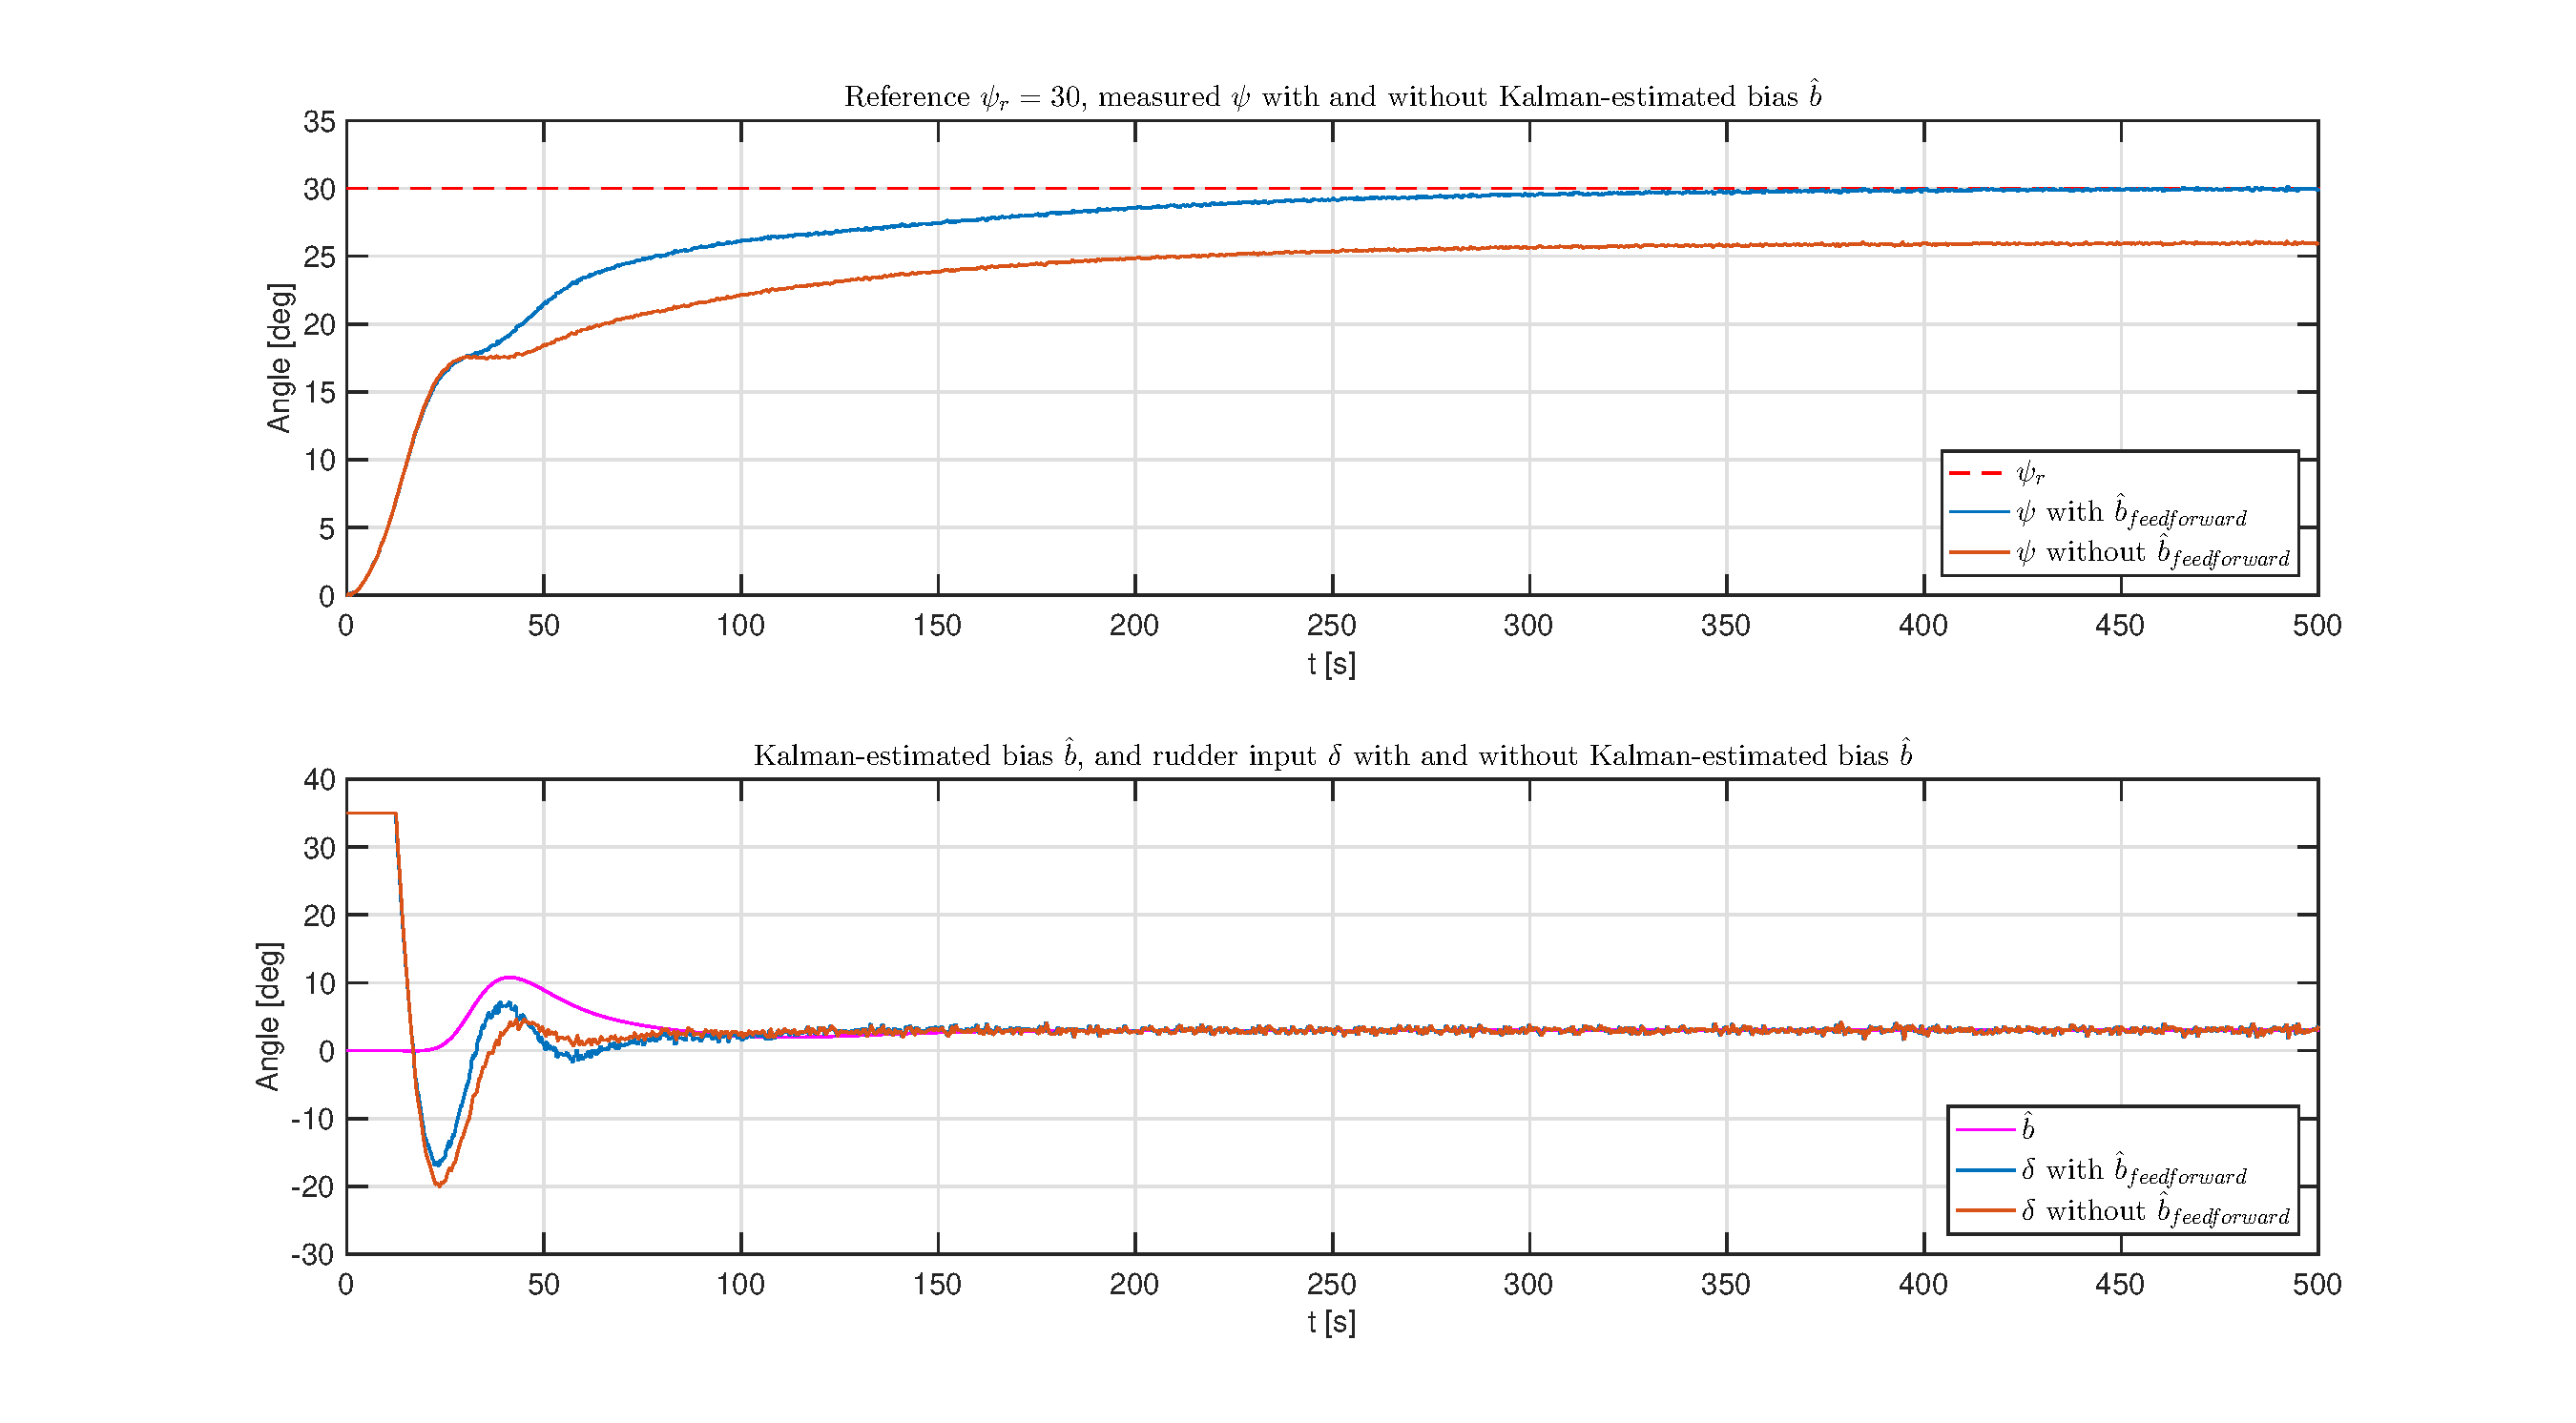
\includegraphics[scale=0.45]{plots/5d}}
    \label{plot:5d}
\end{figure}

\newpage
\begin{figure}[!htb]
    \caption{North-East plot of ship course with and without Kalman}
    \centering
     \centerline{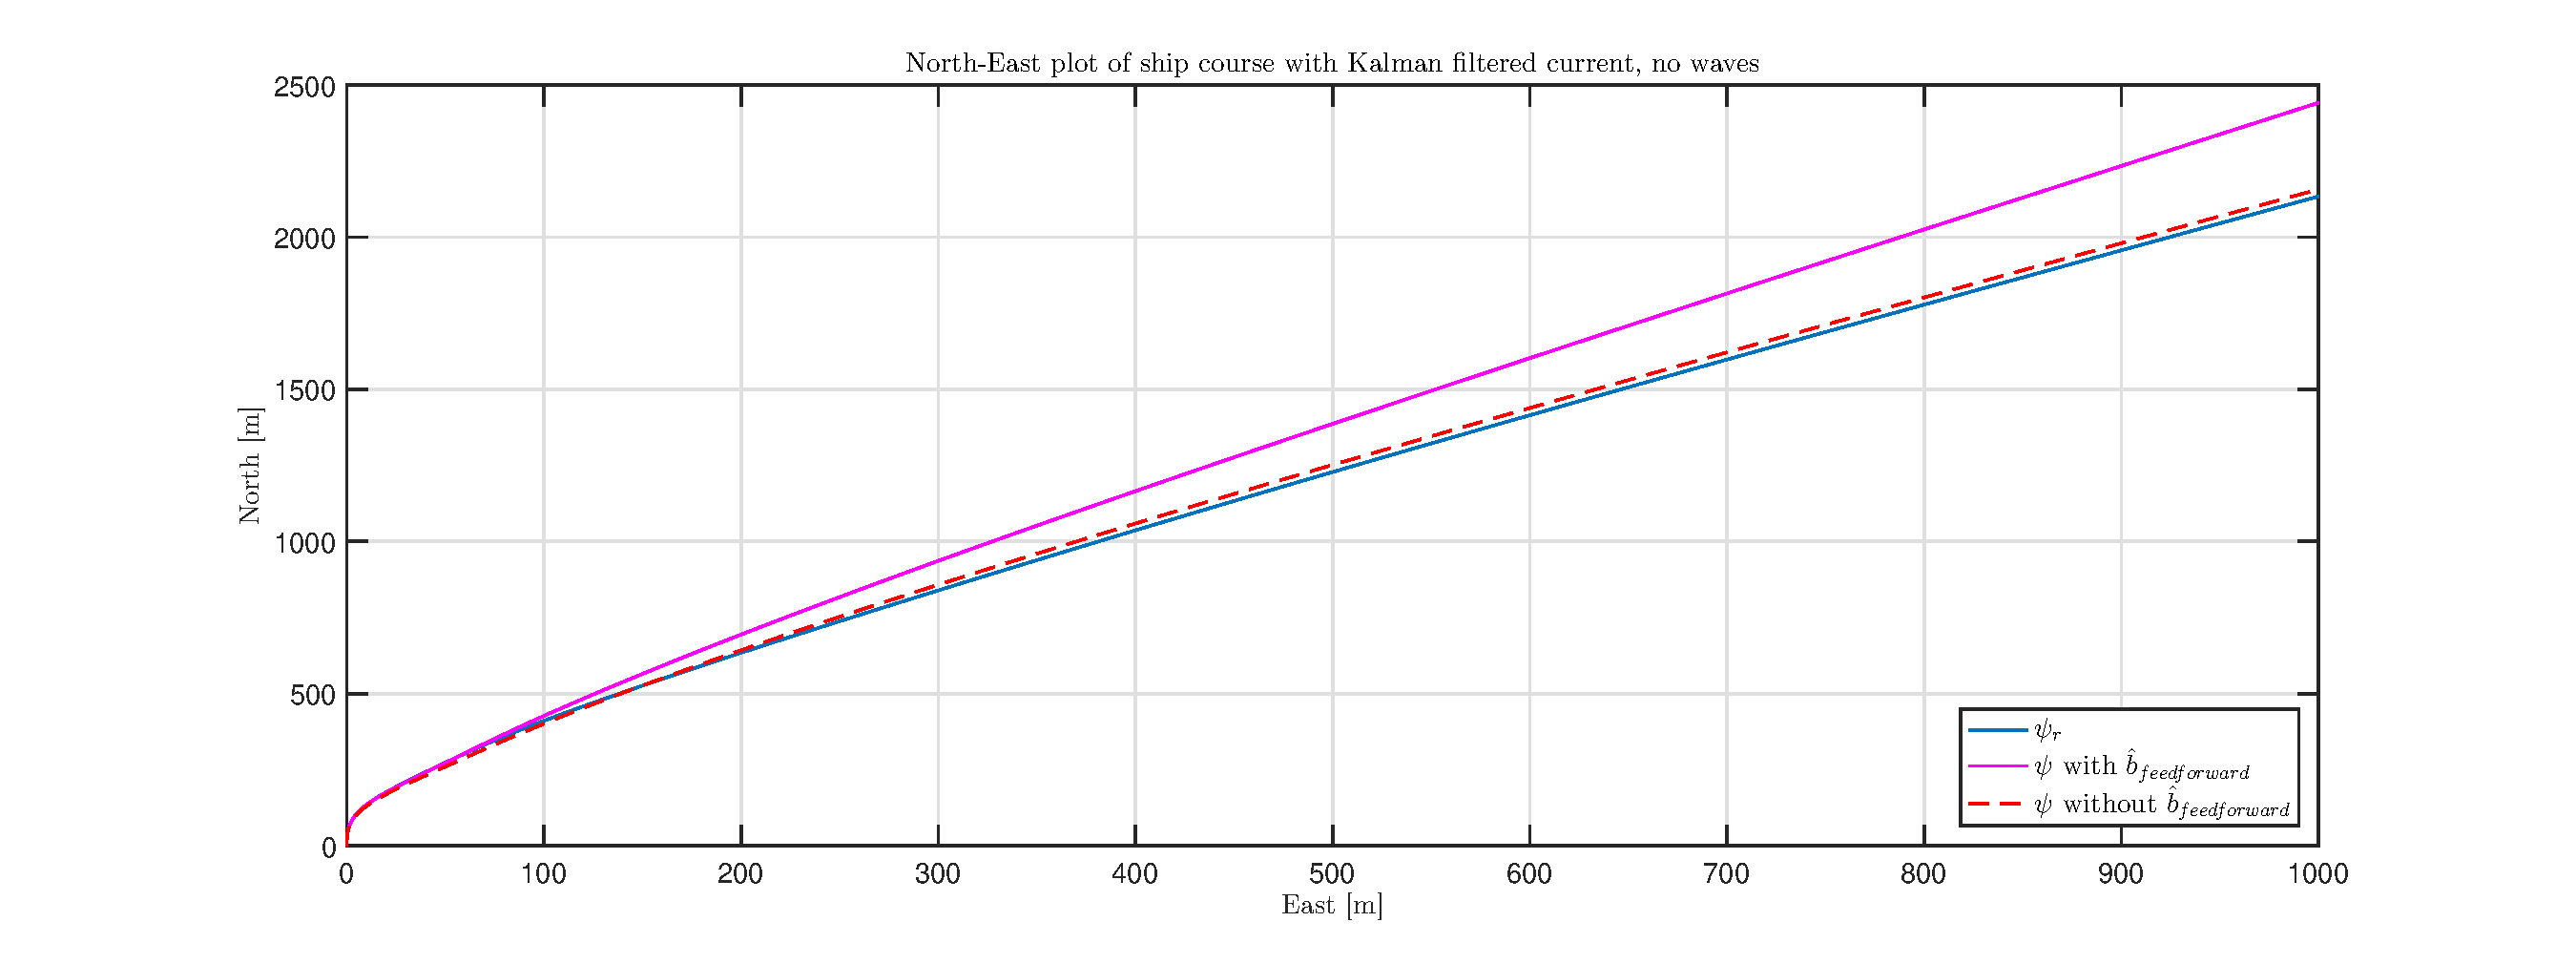
\includegraphics[scale=0.45]{plots/5eORd}}
    \label{plot:5d}
\end{figure}


%%%%%%%%%%%%%%%%%%%%%%%%%%%%%%%%%%%%%%%%%%%
% 5.5 Wave filtering
%%%%%%%%%%%%%%%%%%%%%%%%%%%%%%%%%%%%%%%%%%%
\subsection{Wave filtering}

In this section, the estimated heading $\hat \psi $ will be used instead of the measured heading for the feedback in the autopilot, in addition to the feed forward from the estimated bias. This system is also simulated with ${\psi _r} = 30$, but now with both current and wave disturbances applied.
From Figure 13 we can see the estimated compass $\hat{\psi}$ and the measured compass $\psi$, with the estimated having much less oscillations. In Figure 14 we can see the rudder input and estimated bias, with and without Kalman. Figure 15 shows the heading of the ship with and without Kalman, while Figure 16 shows that the wave bias estimator follows the measured bias, meaning we have a good estimator. 

\begin{figure}[!htb]
    \caption{Measured compass and estimated compass}
    \centering
    \centerline{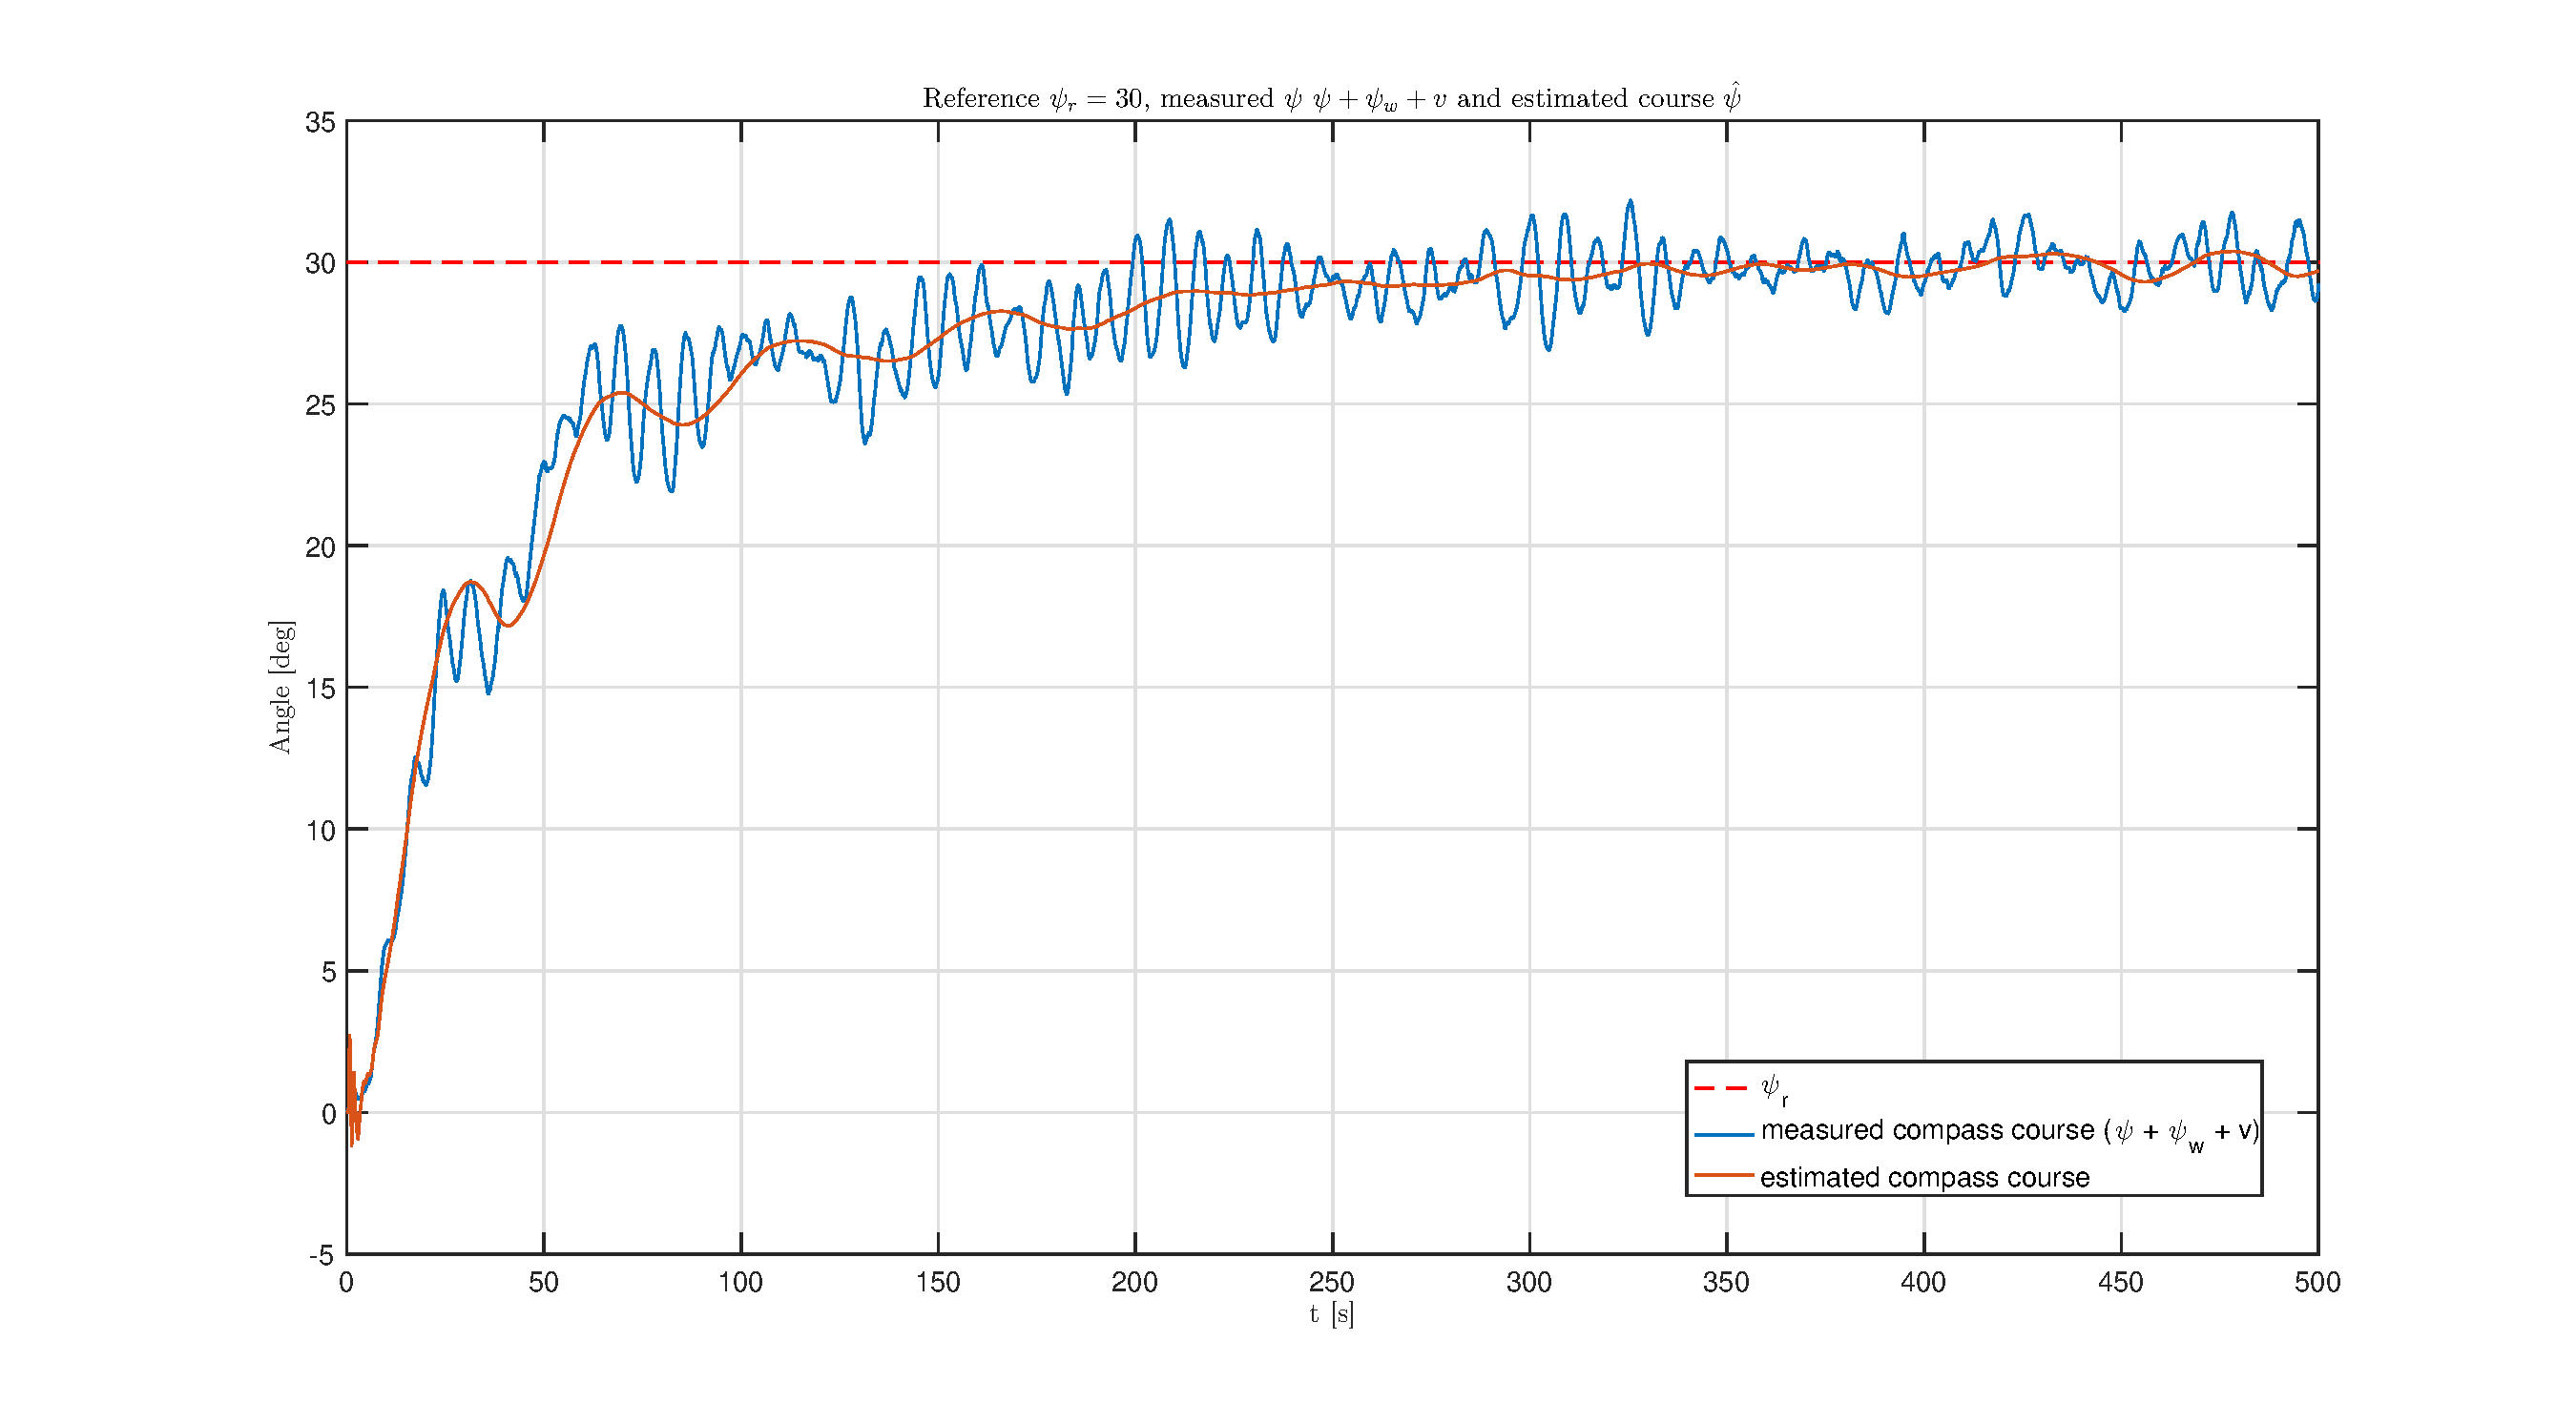
\includegraphics[scale=0.25]{plots/5e5}}
    \label{plot:5e1}
\end{figure}


\begin{figure}[!htb]
    \caption{Rudder input and estimated bias}
    \centering
    \centerline{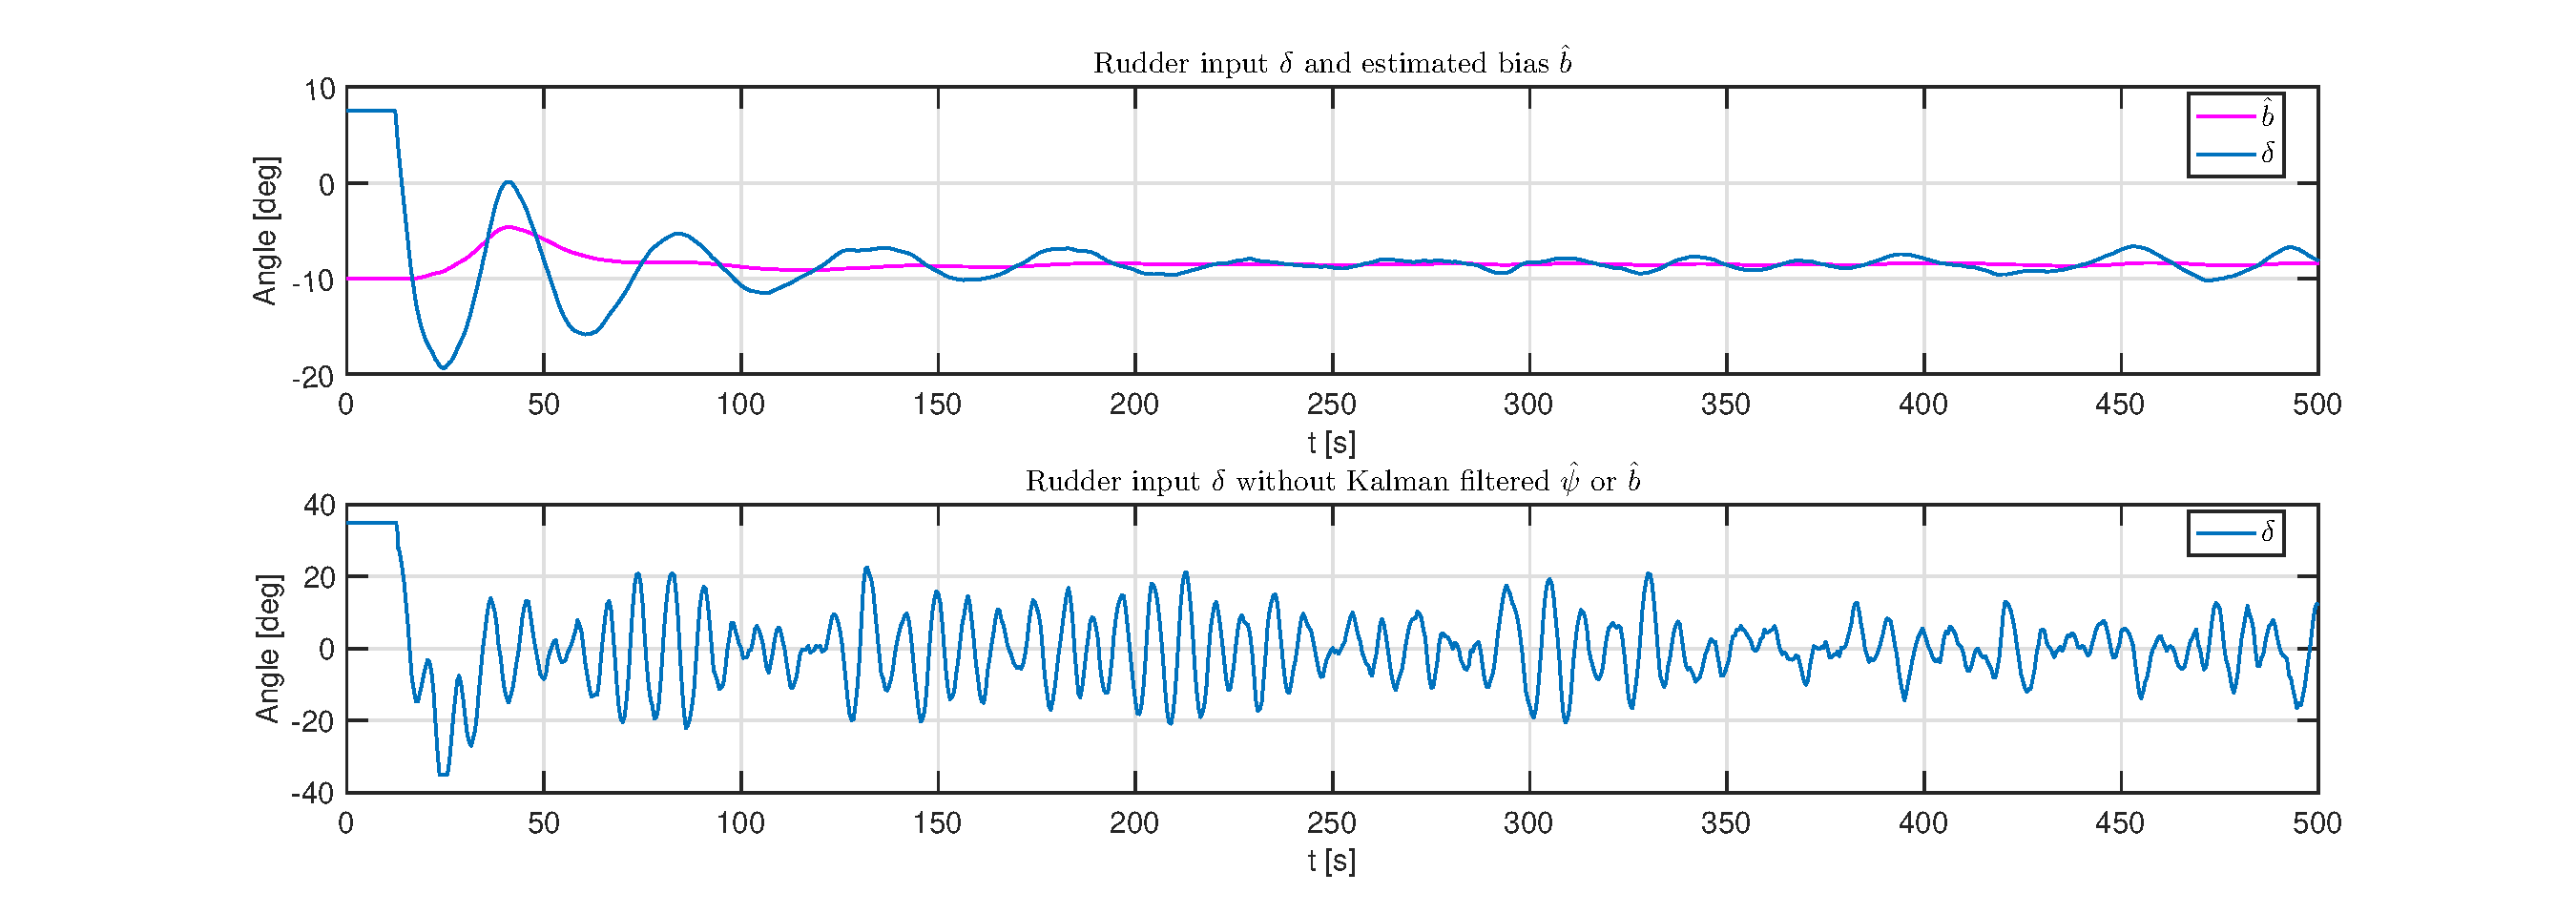
\includegraphics[scale=0.40]{plots/5e1}}
    \label{plot:5e1}
\end{figure}

\begin{figure}[!htb]
    \caption{North-East plot with Kalman filtered current and waves}
    \centering
    \centerline{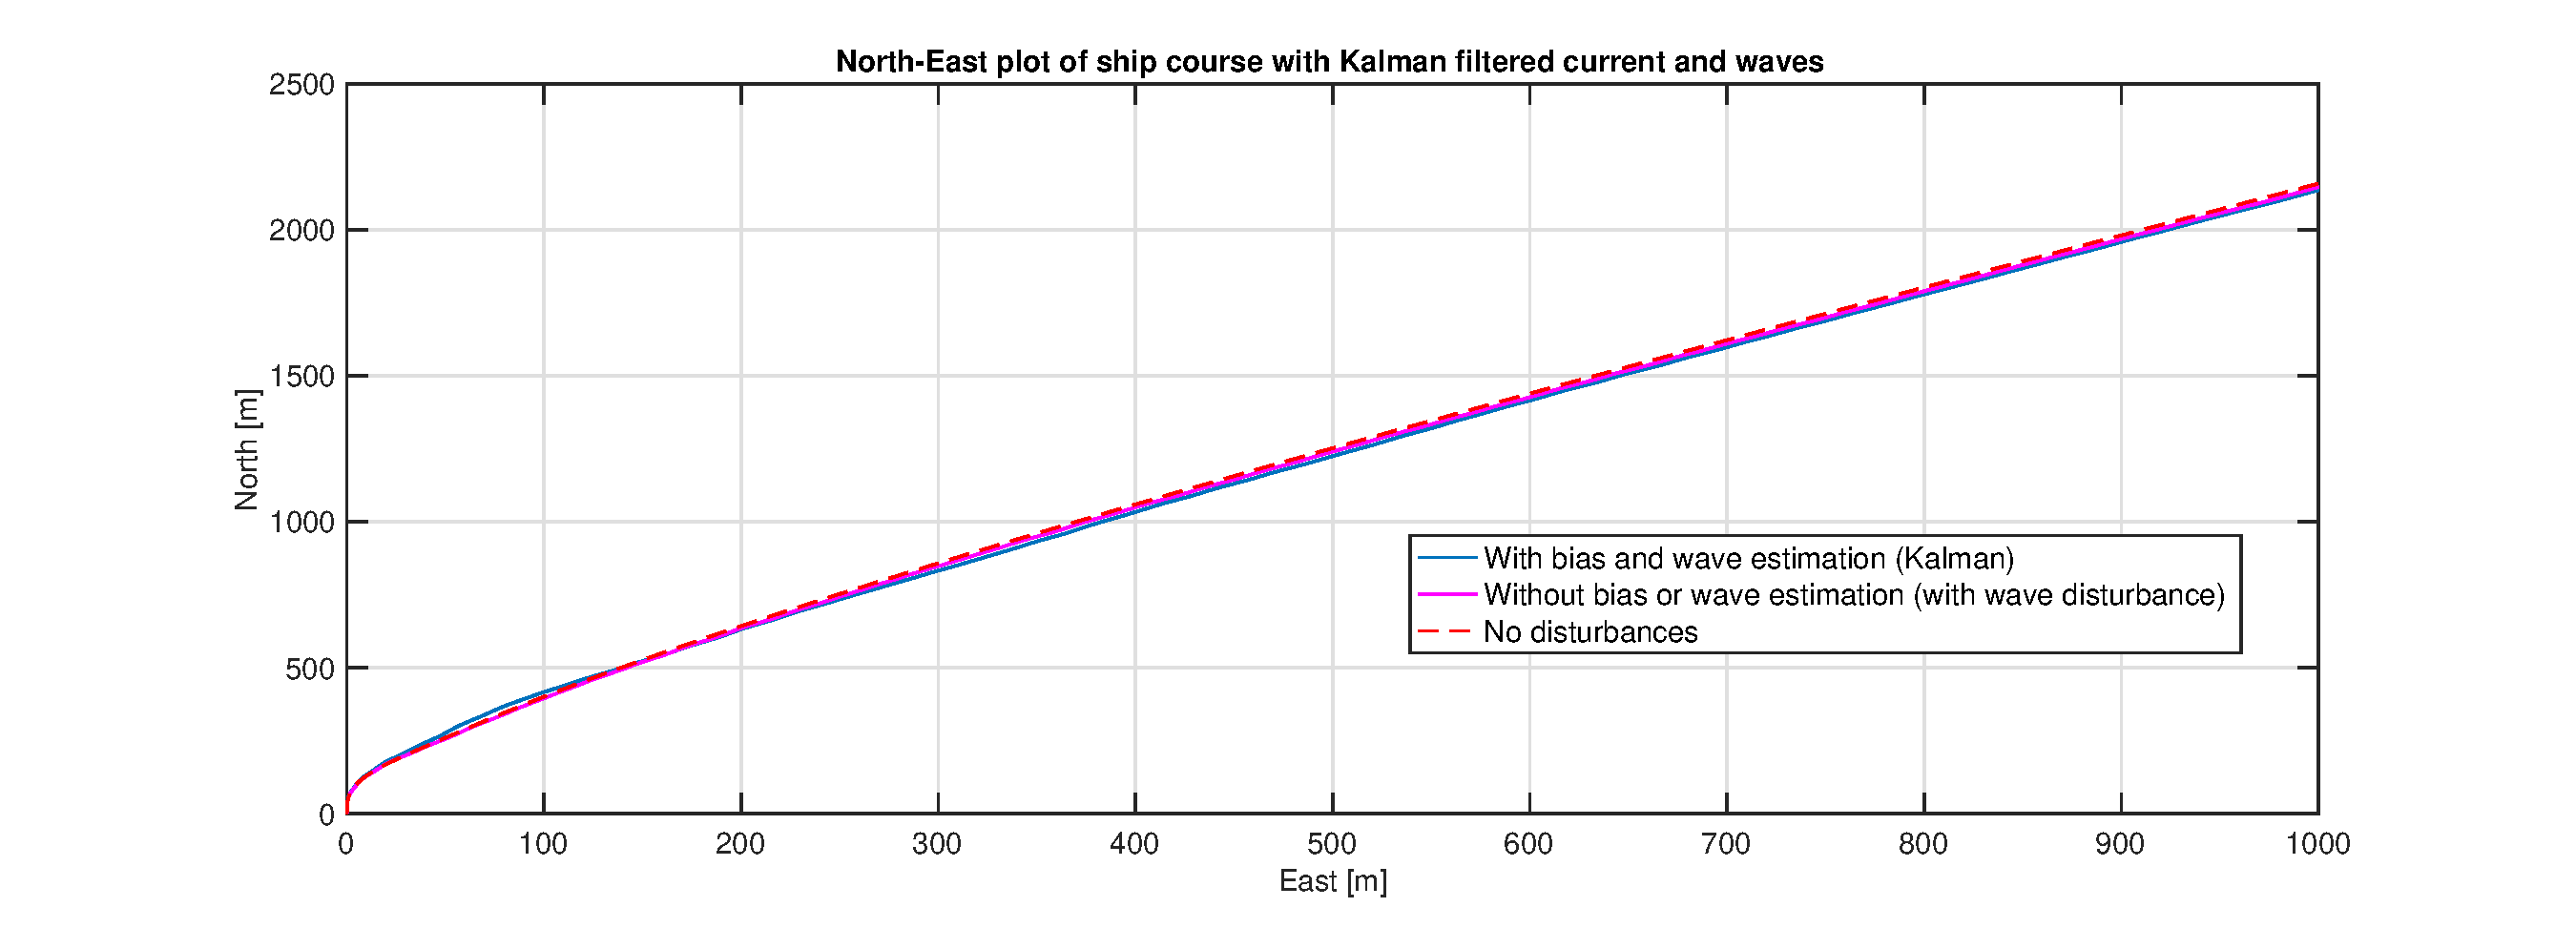
\includegraphics[scale=0.35]{plots/5e2}}
    \label{plot:5e2}
\end{figure}

\begin{figure}[!htb]
    \caption{Wave influence}
    \centering
    \centerline{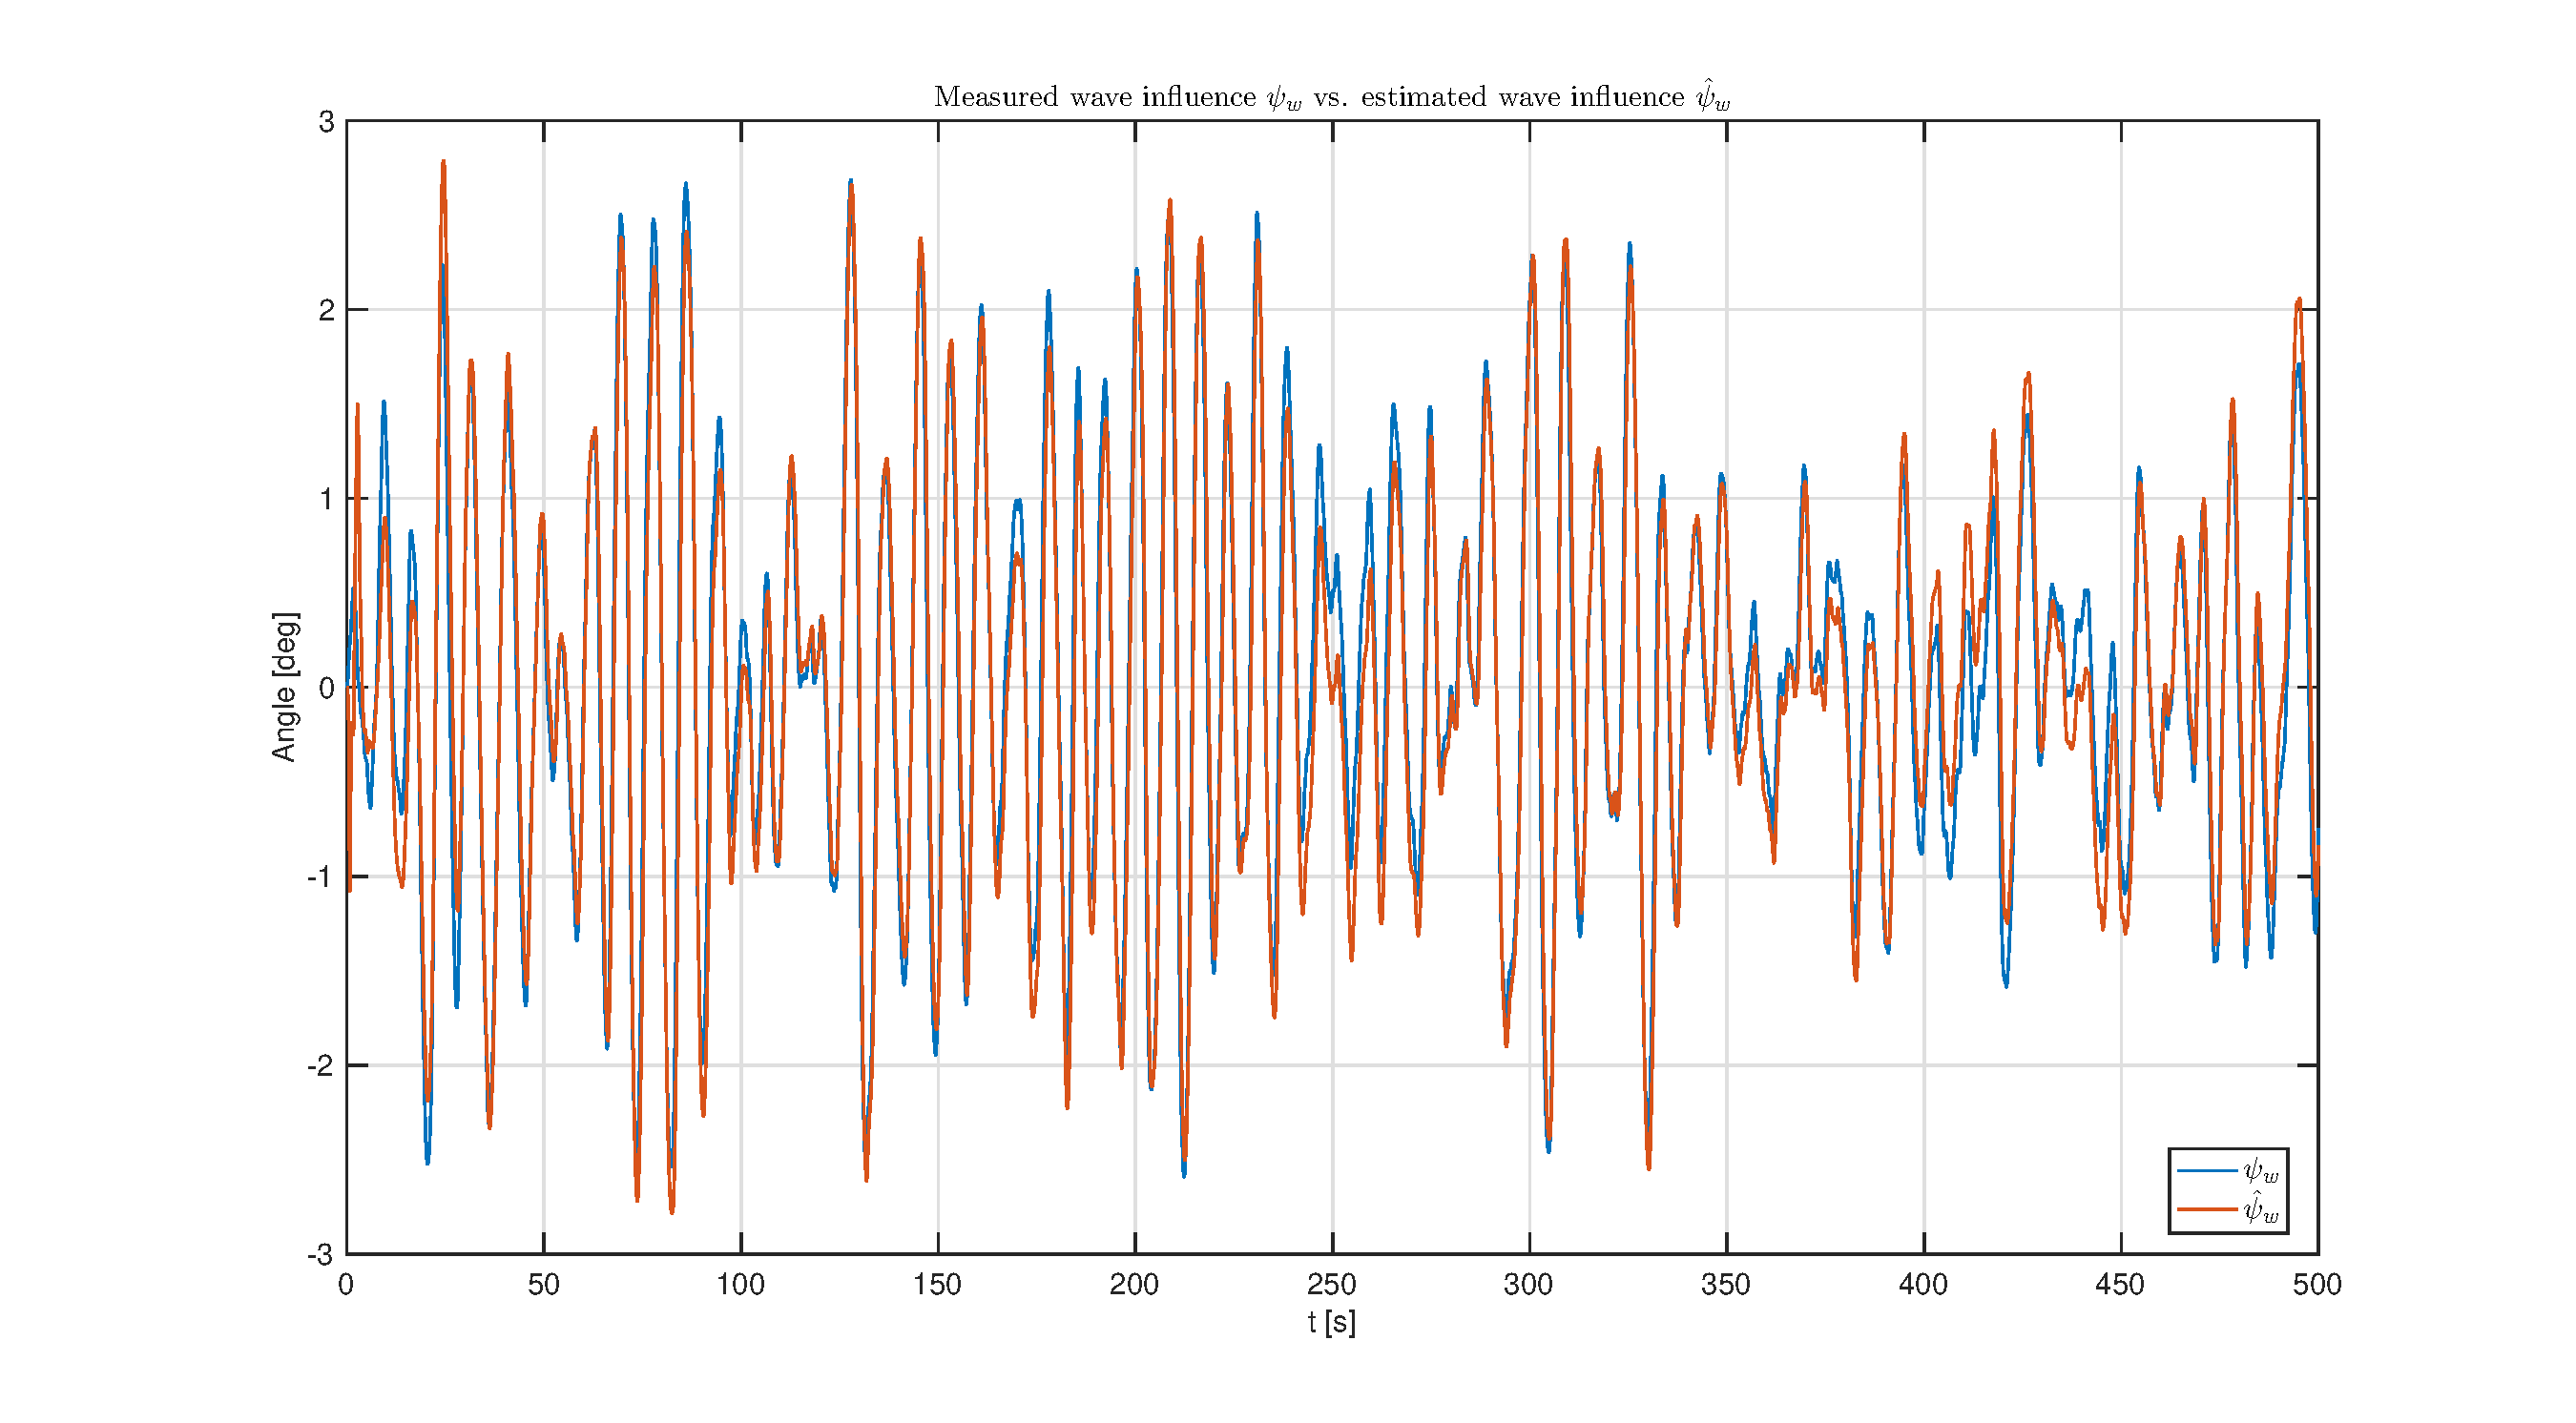
\includegraphics[scale=0.30]{plots/5e3}}
    \label{plot:5e3}
\end{figure}

\newpage\null\thispagestyle{empty}\newpage
\newpage\null\thispagestyle{empty}\newpage
\newpage
\section{Conclusion}

After identifying model parameters in section 1, we were able to develop a feasible approximation of the ship model. By analyzing the input and output responses, a ship model with measurement noise, wave disturbance and current disturbance were developed. 

The implementation of the discrete Kalman filter was intended for improvement of the control of the ship. To make this implementation possible, we identified the necessary wave base frequency $\omega_{0}$ and the wave damping factor $\lambda$ in section 2. Figure \ref{plot:2d} shows that the analytically derived and the estimated PSD functions cohere. 

A PD controller is designed in section 3 to keep angle of the heading at a desired value. Tuning of this particular controller is done so that the damping part cancels the ship time constant, putting the pgase margin and cut-off frequency values respectively to $\phi  = {50^o}$ and ${\omega _c} = 0.1\frac{{rad}}{s}$. These characteristics are proved in figure \ref{plot:3a}.

In section 4 we check the observability of the system. This is done by transforming the system into state-space form, and calculating the observability matrices in MatLab. After checking the rank of each observability matrix in section 4, we could declare the system observable independent of the composition of disturbances.

The final part of this assignment was completed in section 5, where a discrete Kalman filter is applied. This was done through discretization of the system using MatLab before the Kalman filter was implemented using a Matlab function within the Matlab Simulink Block with persistent variables, according to Appendix B in the assignment text.
\newpage
\section{Appendix A: MatLab Code}

\subsection{Part 1 - Identification of boat parameters}
\begin{lstlisting}
%% 1b Simulating in calm water(no disturbances) and identification of parameter T and K
omega = 0.005; %rad/s w_1
A=1;           %Amplitude
simTime = 1000; % [s]
simout = sim('ship1b','startTime','0','stopTime',sprintf('%d',simTime));
time = simout.get('time');     %get time from workspace
psi_w1 = simout.get('psi'); %get psi from workspace

% run the simulation with  w_2
omega = 0.05; %[rad/s] w_2
A=1;          %Amplitude

simTime = 1000; % [s]
simout = sim('ship1b','startTime','0','stopTime',sprintf('%d',simTime));
time = simout.get('time');     %get time from workspace
psi_w2 = simout.get('psi'); %get psi from workspace

%plotting into one window
subplot(2,1,1)
plot(time,psi_w1)
xlabel('t [s]')
ylabel('$\psi$ [deg]')
title('Simulation with $\omega_1=0.005$   (No Noise on measurement)')
legend('\psi (average heading) ', 'Location','SouthEast')
grid on;
subplot(2,1,2)
plot(time,psi_w2)
xlabel('t [s]')
ylabel('$\psi$ [deg]')
title('Simulation with $\omega_w=0.05$   (No Noise on measurement)')
legend('\psi (average heading) ', 'Location','SouthEast')
grid on;

%%code that identifies the T and K value


%% 1c: Simulating in rough weather(Waves+Noise) Amplitude=1
omega = 0.005; %rad/s %w_1
A=1;           %Amplitude
simTime = 1000; % [s]
simout = sim('ship1c','startTime','0','stopTime',sprintf('%d',simTime));
time = simout.get('time');     %get time from workspace
psi_w1_rough = simout.get('psi'); %get psi from workspace

%simulate again for w_2
omega = 0.05;  %rad/s %w_w
A=1;           %Amplitude
simTime = 1000; % [s]
simout = sim('ship1c','startTime','0','stopTime',sprintf('%d',simTime));
time = simout.get('time');     %get time from workspace
psi_w2_rough = simout.get('psi'); %get psi from workspace

%Ploting the figures
subplot(2,1,1)
plot(time,psi_w1_rough)
xlabel('t [s]')
ylabel('$\psi$ [deg]')
title('Simulation with $\omega_1=0.005$  (With waves and measurement noise) ')
legend('\psi + \psi_{w} (average heading +  wave disturbances) ', 'Location','SouthEast')
grid on;
subplot(2,1,2)
plot(time,psi_w2_rough)
xlabel('t [s]')
ylabel('$\psi$ [deg]')
title('Simulation with $\omega_w=0.05$   (With waves and measurement noise)')
legend('\psi + \psi_{w} (average heading +  wave disturbances) ', 'Location','SouthEast')
grid on;


%% 1c: simulation in rough weather (waves+noise) with higher amplitude A=45

omega = 0.005; %rad/s %w_1
A=45;           %Amplitude
simTime = 1000; % [s]
simout = sim('ship1c','startTime','0','stopTime',sprintf('%d',simTime));
time = simout.get('time');     %get time from workspace
psi_w1_rough_A45 = simout.get('psi'); %get psi from workspace

%simulate again for w_2
omega = 0.05;  %rad/s %w_w
A=45;           %Amplitude
simTime = 1000; % [s]
simout = sim('ship1c','startTime','0','stopTime',sprintf('%d',simTime));
time = simout.get('time');     %get time from workspace
psi_w2_rough_A45 = simout.get('psi'); %get psi from workspace

%Plotting the figures
subplot(2,1,1)
plot(time,psi_w1_rough_A45)
xlabel('t [s]')
ylabel('$\psi$ [deg]')
title('Simulation with $\omega_1=0.005$ and $A=45$   (With waves and measurment noise) ')
legend('\psi + \psi_{w} (average heading +  wave disturbances) ', 'Location','SouthEast')
grid on;
subplot(2,1,2)
plot(time,psi_w2_rough_A45)
xlabel('t [s]')
ylabel('$\psi$ [deg]')
title('Simulation with $\omega_w=0.05$ and $A=45$   (With waves and measurment noise)')
legend('\psi + \psi_{w} (average heading +  wave disturbances) ', 'Location','SouthEast')
grid on;

%% 1d: Comparison of all models
%Make The Transfer Functions 
num1=[0.1742];       %with K
den1=[86.52685 1 0]; %with T
H1=tf(num1,den1);    %No noise Transfer Function

num2=[0.1734];       %with K
den2=[84.3920 1 0];  %with T
H2=tf(num2,den2);    %With noise Transfer Function

%simulate
simTime = 1000; % [s]
simout = sim('ship1d','startTime','0','stopTime',sprintf('%d',simTime));
time = simout.get('time');
psi_s = simout.get('psi'); %system
psi_no_noise = simout.get('psi_no_noise'); %model with no noise
psi_with_noise = simout.get('psi_with_noise'); %model with noise

%draw plot
plot(time,psi_s,'r',time,psi_with_noise,'b',time,psi_no_noise,'g')
xlabel('t [s]')
ylabel('$\psi$ [deg]')
legend('Ship','Model (calm)','Model (rough)','Location','southeast')
title('Step response of models and system')
grid on
\end{lstlisting}

\subsection{Part 2 - Identification of wave spectrum model}
\begin{lstlisting}
%% 2a: Estimate PSD
load('wave.mat');       % Load wave disturbance

F_s = 10;
window = 4096;
noverlap = [];
nfft = [];
[S_psi,f] = pwelch(psi_w(2,:).*(pi/180),window,noverlap,nfft,F_s);
omega = 2*pi.*f;
S_psi = S_psi./(2*pi);


%% 2c: Find omega_0
% Plot estimated PSD

plot(omega,S_psi, 'LineWidth', 2)
axis([0 2 -0.00005 16*10^(-4)])
hold on
xlabel('$\omega$ [$\frac{rad}{s}$]')
ylabel('$S_{\psi_{w}}(\omega)$ [rad]')
title(['Estimated power spectral density fuction of $S_{\psi_{w}}(\omega)$ '...
    ])
grid on;


%% 2c: Find resonance frequency from estimated PSD)
[maxPSD,  frequency_index ] = max( S_psi )
omega_0 = omega( frequency_index )

%% 2d: Comparison
sigma = sqrt(maxPSD); % sigma_squared is the peak value of S_psi_w

%using lsqcurvefit

P_psi = @(lambda,omega) ...
    (4*lambda^2*omega_0^2*sigma^2*omega.^2) ./ ...
    (omega.^4 + (2*lambda^2 - 1)*2*omega_0^2*omega.^2 + ...
    omega_0^4);

lambda0 = 10;
lb=0;
ub=10;

lambda = lsqcurvefit(P_psi,lambda0,omega,S_psi,lb,ub);
P_psi = P_psi(lambda,omega);
K_w = 2*lambda*omega_0*maxPSD;

%%% Comparison plot of estimate and analytical
figure
plot(omega, P_psi, 'r')
hold on
plot(omega, S_psi, 'b')
legend('P_{\psi_w}','S_{\psi_w}')
xlim([0 2])
xlabel('t [s]')
ylabel('PSD [deg^2/(rad/s)')
title('Comparison of estimated PSD function $(S_{\psi_w})$ and the analytical $P_{\psi_w}$');
grid on;

\end{lstlisting}

\subsection{Part 3 - Control system design}
\begin{lstlisting}
%%From earlier excercies 
K=0.1734;
T=84.3920;
%% 5.3a
w_c=0.1; %cutoff frequency [rad/s]
PM=50/180*pi;%Phase margin [rad]
T_d=T;        %chosen such that it cancels the TF time constant
%Make transfer function for controller
T_f=1/(tan(PM)*w_c);    
K_pd=sqrt((T_f^2*w_c^4+w_c^2)/K^2);
num_controller=[K_pd*T_d,K_pd];
den_controller=[T_f,1];

H_pd=tf(num_controller,den_controller); %make transfer function for controller

%%Make transfer function for plant
H_ship=tf([K],[T 1 0]);                 %transfer function for plant

%open-loop system
H_ol=H_pd*H_ship;                       %Open loop transfer function

%draw a bode idagram
figure
bode(H_ol);
grid ;
title('Bode plot for the open-loop system H_ol(s)');



%% 5.3b)

ref=30;
simTime=400; 

simout = sim('ship3b','startTime','0','stopTime',sprintf('%d',simTime));
time = simout.get('time');     %get time from workspace
psi = simout.get('psi'); %get psi from workspace
ref=simout.get('ref');
%error=simout.get('error'); % no need for this, not gonna plot it.
delta=simout.get('rudder_input');

%Ploting the graphs
figure
plot(time,ref,'black--',time,psi,time,delta) %plots time against refrence, output and rudder_input
legend('\psi_r(t)','\psi(t)','\delta(t)','location','Southeast')
xlabel('t[s]');
ylabel('\psi_r(t), \psi(t), \delta(t) [deg]'); 
title('Autopilot without current or wave disturbances')
%make y-axis formating become less
grid on;

%% 5.3c)

ref=30;
simTime=400; 

simout = sim('ship3c','startTime','0','stopTime',sprintf('%d',simTime));
time = simout.get('time');     %get time from workspace
psi = simout.get('psi'); %get psi from workspace
ref=simout.get('ref');
%error=simout.get('error'); % no need for this, not gonna plot it.
delta=simout.get('rudder_input');

%Ploting the graphs
figure
plot(time,ref,'black--',time,psi,time,delta) %plots time against refrence, output and rudder_input
legend('\psi_r(t)','\psi(t)','\delta(t)','location','Southeast')
xlabel('t[s]');
ylabel('\psi_r(t), \psi(t), \delta(t) [deg]'); 
title('Autopilot with current disturbances')
%make y-axis formating become less
grid on;

%% 5.3d)

ref=30;
simTime=400; 

simout = sim('ship3d','startTime','0','stopTime',sprintf('%d',simTime));
time = simout.get('time');     %get time from workspace
psi = simout.get('psi'); %get psi from workspace
ref=simout.get('ref');
%error=simout.get('error'); % no need for this, not gonna plot it.
delta=simout.get('rudder_input');

%Ploting the graphs
figure
plot(time,ref,'black--',time,psi,time,delta) %plots time against refrence, output and rudder_input
legend('\psi_r(t)','\psi(t)','\delta(t)','location','Southeast')
xlabel('t[s]');
ylabel('\psi_r(t), \psi(t), \delta(t) [deg]'); 
title('Autopilot with wave disturbances')
%make y-axis formating become less
grid on;


\end{lstlisting}

\subsection{Part 4- Observability}
\begin{lstlisting}
load('constants');
%% 5.4a): Finding the matrices
A = [0 1 0 0 0; -omega_0^2 -2*lambda*omega_0 0 0 0; 0 0 0 1 0; ...
    0 0 0 -1/T -K/T; 0 0 0 0 0];
B = [0; 0; 0; K/T; 0];
C = [0 1 1 0 0];
E = [0 0; K_w 0; 0 0; 0 0; 0 1];

%% 5.4b): Observabillity without disturbances
A = [0 1; 0 -1/T];
B=[0; K/T];
C= [1 0];
O = obsv(A,C);
rank(O) % rank(O) = 2 == n -> observable

%% 5.4c) Observabillity with current
A_b = [0 1 0; 0 -1/T -K/T; 0 0 0]; 
C_b = [1 0 0];
O_b = obsv(A_b,C_b);
rank(O_b)   %rank(O_b) = 3 == n -> observable


%% 5.4d) Observabillity with waves 
A_w = [0 1 0 0; -omega_0^2 -2*lambda*omega_0 0 0; 0 0 0 1; 0 0 0 -1/T];
C_w = [0 1 1 0];
O_w = obsv(A_w,C_w);
rank(O_w) % rank(Ob) = 4 == n -> observable

%% 5.4e) Observabillity with current and wave
O_cw = obsv(A,C); % rank(Ob) = 5 == n -> observable

\end{lstlisting}

%%%%%%%%%%%%%%%%%%%%%%%%%%%%%%%%%%%%%%%%%%%%%%%%%%%%%%%%%%%%%%%%%%%%%%%%%%%%%%%%%%%%%%%%%%%%%
% PART 5 - DISCRETE KALMAN FILTER
%%%%%%%%%%%%%%%%%%%%%%%%%%%%%%%%%%%%%%%%%%%%%%%%%%%%%%%%%%%%%%%%%%%%%%%%%%%%%%%%%%%%%%%%%%%%%

\subsection{Part 5 - Discrete Kalman filter function}

\begin{lstlisting}
function [b,psi] = fcn(u, y, data)

persistent init_flag A B C E Q R P_ x_ I 

if (isempty(init_flag))
    init_flag = 1;
    
    % Initialization for system
    [A,B,C,E,Q,R,P_,x_, I] = deal(data.Ad,data.Bd,data.Cd,data.Ed,data.Q, ...
                                data.R, data.P_0, data.X_0, data.I);
end

% 1 - Compute the Kalman Gain
    L = (P_*C')/((C*P_*C'+R));
% 2 - Update estimate with measurment
    x = x_ + L*(y-C*x_);
% 3 - Update error covariance matrix
    P = (I - L*C)*P_*(I-L*C)'+L*R*L';
% 4 - go to next
    x_ = A*x + B*u;
    P_ = A*P*A' + E*Q*E';

psi = x(3); b = x(5);
\end{lstlisting}

\begin{lstlisting}
%% 5.1a): 
load('constants');

%Make transfer function for controller
T_f=1/(tan(PM)*w_c);    
K_pd=sqrt((T_f^2*w_c^4+w_c^2)/K^2);
num_controller=[K_pd*T_d,K_pd];
den_controller=[T_f,1];

% Discretize model
A = [0 1 0 0 0; -omega_0^2 -2*lambda*omega_0 0 0 0; 0 0 0 1 0; ...  
    0 0 0 -1/T -K/T; 0 0 0 0 0];
B = [0; 0; 0; K/T; 0];
C = [0 1 1 0 0];
D = 0;
E = [0 0; K_w 0; 0 0; 0 0; 0 1];

f_s=10;         % Sampling frequency [Hz]
T_s = 1/f_s;    % Sampling time [s]

% Discretize model 
[Ad,Bd] = c2d(A,B,T_s);
% Discretize model 
[~,Ed] = c2d(A,E,T_s);
Cd=C;

%% 5b: measure variance 

simTime = 600; % [s]
simout = sim('ship5b','startTime','0','stopTime',sprintf('%d',simTime)); % no noise
psi = simout.get('compass'); 
R = var(psi*pi/180);    

%% 5c: Discrete Kalman Filter

Q = [30 0; 0 10^(-6)];
R = R/T_s;
P_0 = [1 0 0 0 0; 0 0.013 0 0 0; 0 0 pi^2 0 0; 0 0 0 1 0;  0 0 0 0 2.5*10^-4];
X_0 = [0; 0; 0; 0; 0];
I = diag([1 1 1 1 1]);

% data struct to use in matlab function
 data = struct('Ad',Ad,'Bd',Bd,'Cd',Cd,'Ed', Ed, 'Q',Q,'R', R,'P_0',P_0,'X_0',X_0, 'I', I);
 
 
 %% 5d: Feed forward estimated bias
 
load_system('ship5d.slx')
sim('ship5d.slx')

% Plot measured compass with and without estimated bias
figure(figNum)
figNum = figNum+1;
subplot(2,1,1)
plot(time,ref, 'r--', time, compass, time, compass_kalman)
title(['Reference $\psi_{r} = 30$, measured $\psi$ with and'...
' without Kalman-estimated bias $\hat{b}$']);
xlabel('t [s]'); 
ylabel('Angle [deg]');
legend({'$\psi_{r}$', '$\psi$ with $\hat{b}_{feedforward}$', ...
    '$\psi$ without $\hat{b}_{feedforward}$'},   ...
    'Interpreter', 'latex', 'Location', 'best')
grid  on ;

subplot(2,1,2)
plot(time, bias,'m', time, rudder_input, time, rudder_input_2)
title(['Kalman-estimated bias $\hat{b}$, and rudder input $\delta$ ' ...
'with and without Kalman-estimated bias $\hat{b}$'], ...
 'Interpreter', 'latex');
xlabel('t [s]');
ylabel('Angle [deg]');
legend({'$\hat{b}$', '$\delta$ with $\hat{b}_{feedforward}$', ...
    '$\delta$ without $\hat{b}_{feedforward}$'},   ...
    'Interpreter', 'latex', 'Location', 'best')
grid on;


%% 5e: Feed forward estimated bias and wave filtered psi
load_system('ship5e.slx')
sim('ship5e.slx')


load_system('ship5e.slx')
sim('task5_5_e.slx')

%Plot measured compass and estimated compass
figure(figNum)
figNum = figNum+1;
plot(t,sim_PSI_r, 'r--', t, sim_compass, t, psi_filtered)
title(['Reference $\psi_{r} = 30, measured $\psi$ $\psi + \psi_{w} + v and estimated course \hat{\psi}']);
xlabel('t [s]');
ylabel('Angle [deg]');
legend({'\psi_{r}', 'measured compass course ($\psi$ + $\psi_{w} $+ $v$)' , 'estimated compass course ($\hat{\psi}$)'}, 'Location', 'best')
 grid on; 

 
%Plot measured psi with and without Kalman filtered bias and waves
figure(figNum)
figNum = figNum+1;
plot(t,sim_PSI_r, 'r--', t, sim_compass,'b', t3, psi3,'g')
title('Compass reference \psi_{r} = 30, and measured compass course', ...
   'Interpreter', 'latex');
xlabel('t [s]'); 
ylabel('Angle [deg]');
legend({'$\psi_{r}$', 'With Kalman filtered feedback', ...
    'Without Kalman filtered feedback'},  ...
    'Interpreter', 'latex', 'Location', 'best')
grid on; 

%Plotting delta (rudder input)
figure(figNum)
figNum = figNum+1;
subplot(2,1,1)
plot(time, bias,'m', time,rudder_input)
title('Rudder input $\delta$ and estimated bias $\hat{b}$', ...
     'Interpreter', 'latex');
xlabel('t [s]');
ylabel('Angle [deg]');
legend({'$\hat{b}$', '\delta'},  ...
    'Interpreter', 'latex', 'Location', 'best')
grid on;

subplot(2,1,2)
plot(time, rudder_input)
title(['Rudder input $\delta$ without Kalman filtered $\hat{\psi}$ '...
    'or $\hat{b}$'], 'Interpreter', 'latex');
xlabel('t [s]'); 
ylabel('Angle [deg]');
legend({'$\delta$'}, 'Interpreter', 'latex', 'Location', 'best')
grid on;


% Wave influence (current turned off, delta = 0)
load_system('ship5e_1.slx')  
sim('ship5e_1.slx')

% Plotting wave influence on system
figure(figNum)
figNum = figNum+1;
plot(time, compass, time, compass_kalman)
title(['Measured wave influence \psi_{w} vs. estimated wave influence'...
    ' \hat{\psi}_{w}'],'Interpreter', 'latex');
xlabel('t [s]'); 
ylabel('Angle [deg]');
legend({'$\psi_{w}$', '$\hat{\psi}_{w}$'},  ...
    'Interpreter', 'latex', 'Location', 'best')
grid on;
 
\end{lstlisting}

%%%%%%%%%%%%%%%%%%%%%%%%%%%%%%%%%%%%%%%%%%%%%
% CONTINUE WITH ALL THE MATLAB CODE BEFORE SECTION: SimuLink Models
%%%%%%%%%%%%%%%%%%%%%%%%%%%%%%%%%%%%%%%%%%%%%
\newpage
\section{Appendix B: Simulink Models}

\begin{figure}[!htb]
    \caption{Simulink model from section 1.2/1.3}
    \centering
    \centerline{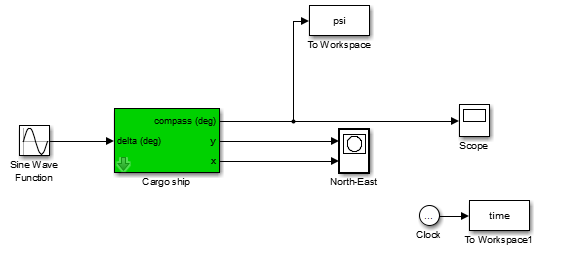
\includegraphics[scale=0.6]{simulink/sim1bc}}
    \label{simulink:1b}
\end{figure}

\begin{figure}[!htb]
    \caption{Simulink model from section 3.3/3.4}
    \centering
    \centerline{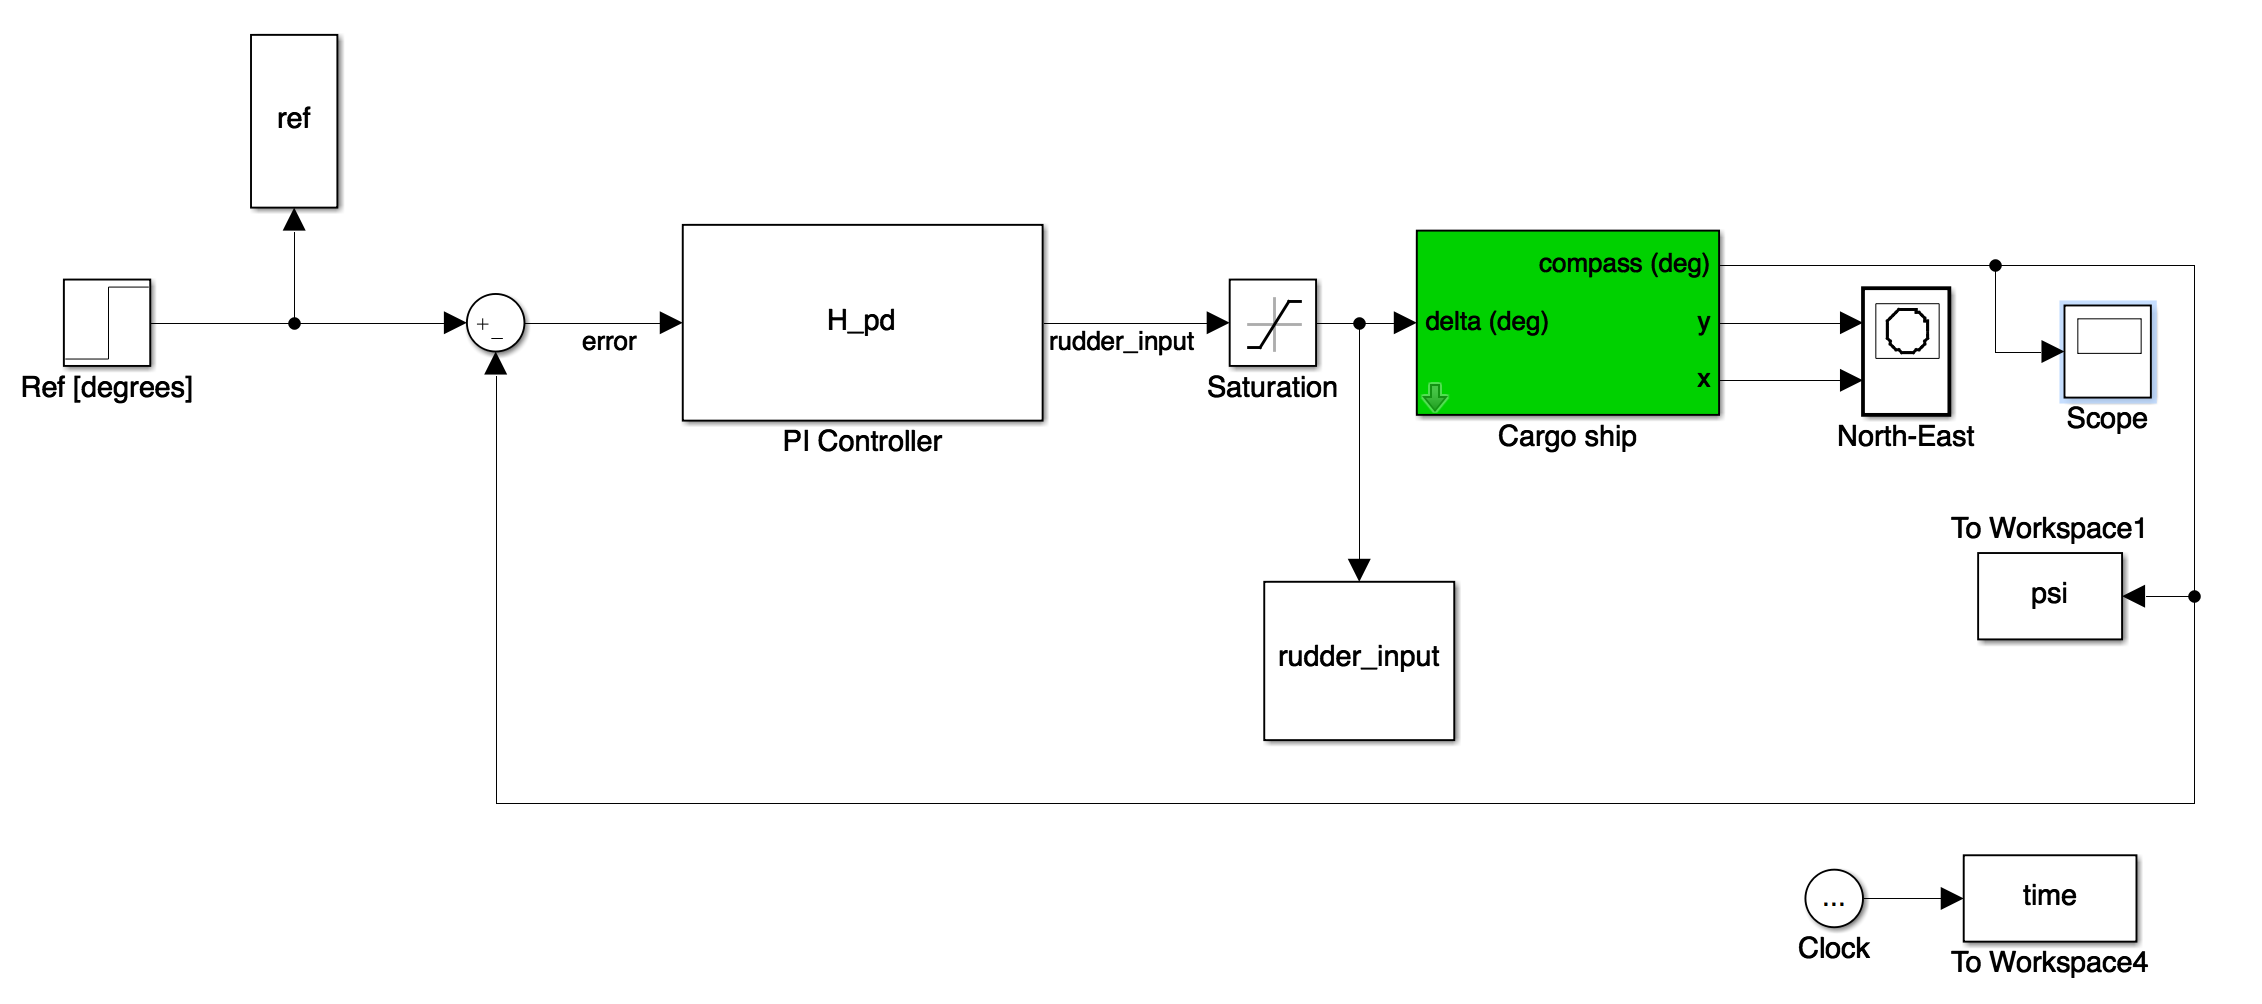
\includegraphics[scale=0.3]{simulink/sim3cd}}

\end{figure}

\begin{figure}[!htb]
    \caption{Simulink model from section 5.2}
    \centering
    \centerline{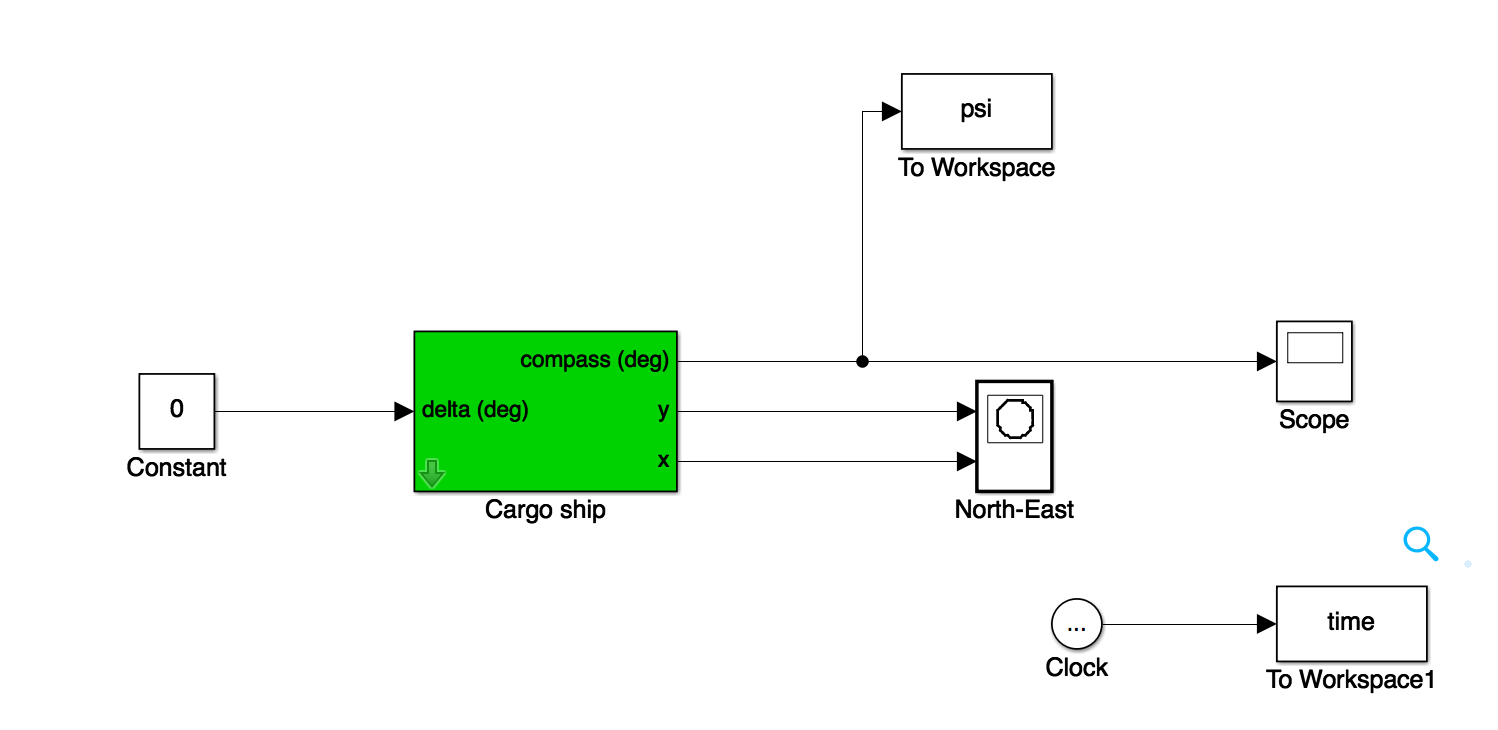
\includegraphics[scale=0.3]{simulink/sim5b}}

\end{figure}

\begin{figure}[!htb]
    \caption{Simulink model from section 5.4}
    \centering
    \centerline{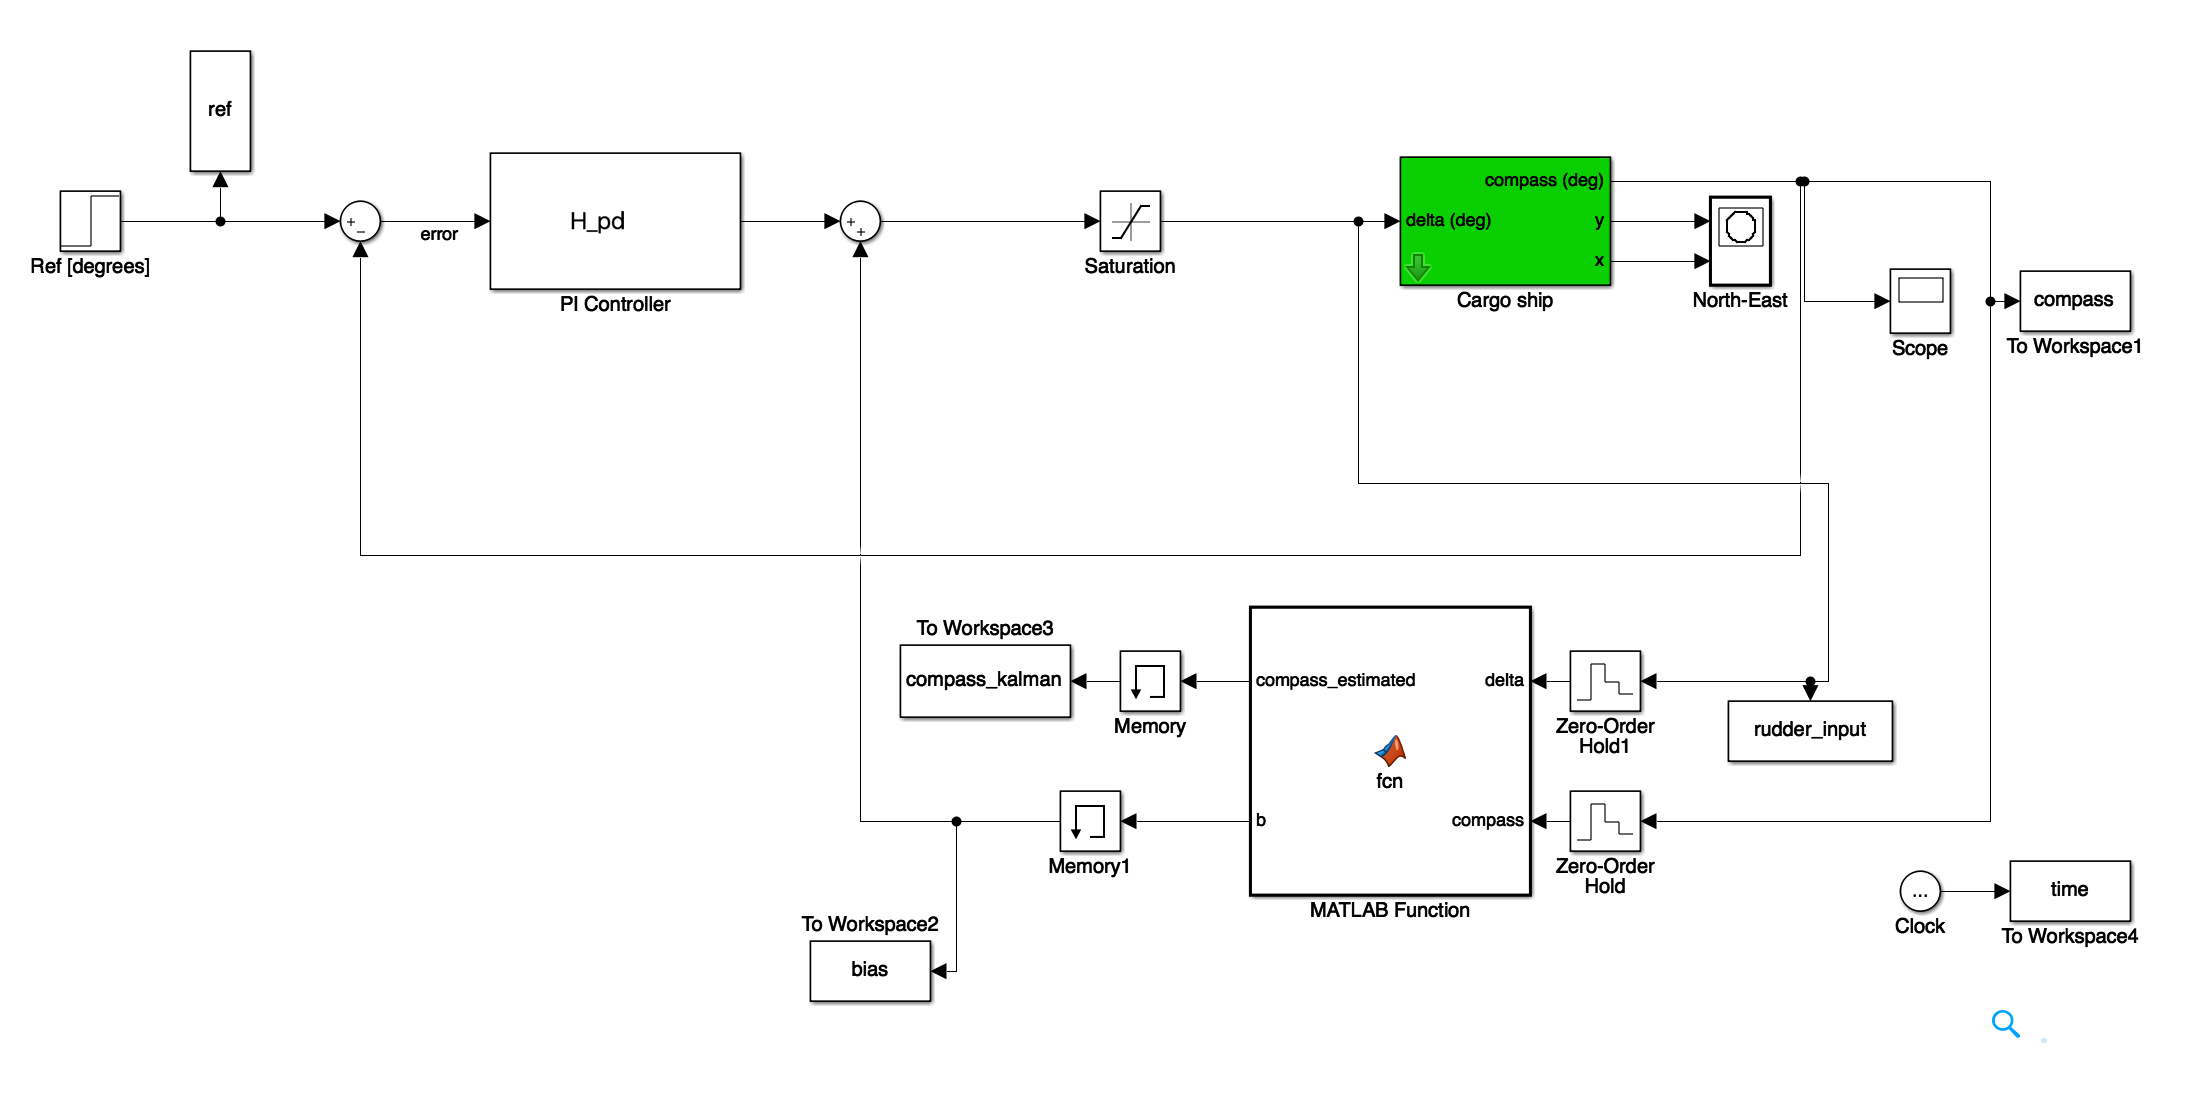
\includegraphics[scale=0.3]{simulink/sim5d}}

\end{figure}

\begin{figure}[!htb]
    \caption{Simulink model from section 5.5}
    \centering
    \centerline{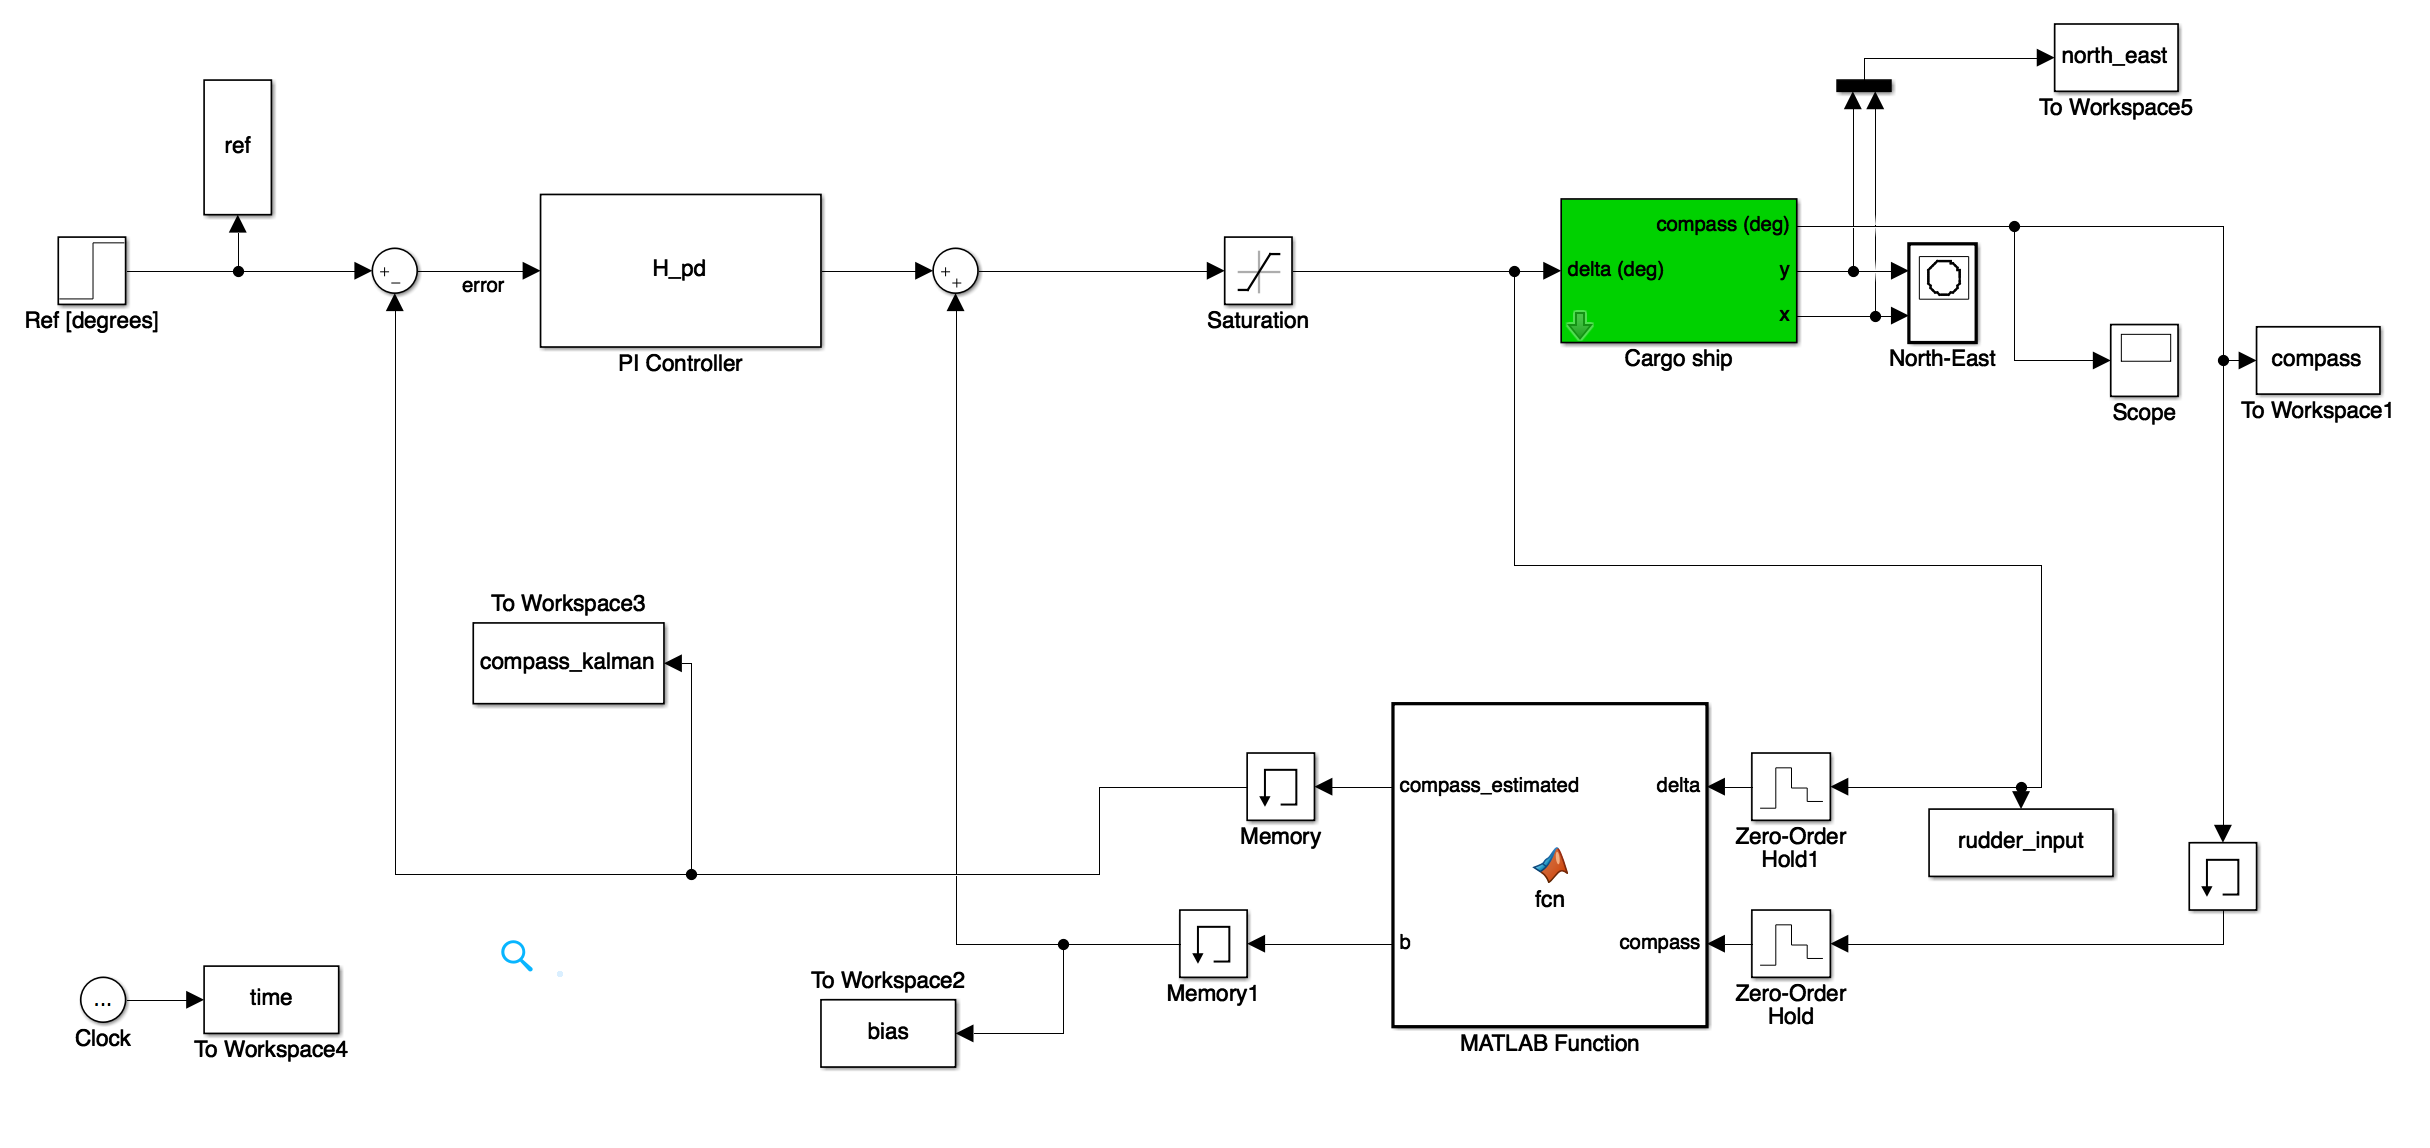
\includegraphics[scale=0.3]{simulink/sim5e}}

\end{figure}



\end{document}
